% Created 2016-11-29 mar. 12:52
% Intended LaTeX compiler: pdflatex
\documentclass[11pt]{article}
\usepackage[utf8]{inputenc}
\usepackage[T1]{fontenc}
\usepackage{graphicx}
\usepackage{grffile}
\usepackage{longtable}
\usepackage{wrapfig}
\usepackage{rotating}
\usepackage[normalem]{ulem}
\usepackage{amsmath}
\usepackage{textcomp}
\usepackage{amssymb}
\usepackage{capt-of}
\usepackage{hyperref}
\usepackage{color}
\usepackage{listings}
\usepackage{syntax}\usepackage{appendix}
\author{Epstein Steven, Rauzy Antoine}
\date{\today}
\title{Open-PSA Model Exchange Format}
\hypersetup{
 pdfauthor={Epstein Steven, Rauzy Antoine},
 pdftitle={Open-PSA Model Exchange Format},
 pdfkeywords={},
 pdfsubject={},
 pdfcreator={Emacs 26.0.50.1 (Org mode 9.0)}, 
 pdflang={English}}
\begin{document}

\maketitle
\tableofcontents

\begin{center}
\begin{tabular}{ll}
Title & Open-PSA Model Exchange Format\\
Version & 2.0d\\
Creation Date & August 1\(^{\text{st}}\), 2007\\
Last modification date & November 28, 2016\\
Editors & Epstein Steven, Rauzy Antoine\\
\end{tabular}
\end{center}


\textbf{Contributors}


This document presents the ``Open-PSA Model Exchange Format''. The
redaction of this representation format is a shared effort. The
following persons contributed to various extents to the current version
of the document: Becker Guenter, Čepin Marko, Contini Sergio, Ducamp
François, Epstein Steven, Herrero Santos Roberto, Hibti Mohamed,
Kampramanis Ioanis, Klügel Jens, Meléndez Asensio Enrique, Perez Mulas
Arturo, Nusbaumer Olivier, Quatrain Richard, Rauzy Antoine, Rauzy Pablo,
Reinhart Mark and Sörman Johan.

\section{The Open-PSA Initiative}
\label{sec:orgc4398d2}



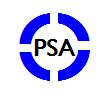
\includegraphics[width=0.9\textwidth]{./word/media/image2.jpeg}

\textbf{The Open Initiative for Next Generation of Probabilistic Safety Assessment}

As we enter a time in which safety and reliability have come to the
attention of the public, especially in the face of climate change and a
nuclear renaissance, efforts are being made in the direction of the
``next generation'' of Probabilistic Safety Assessment with regards to
software and methods. These new initiatives hope to present a more
informative view of the actual models of systems, components, and their
interactions, which helps decision makers to go a step forward with
their decisions.

The Open Initiative for Next Generation PSA provides an open and
transparent public forum to disseminate information, independently
review new ideas, and spread the word. We want to emphasize an openness
which leads to methods and software which have better quality, better
understanding, more flexibility, encourage peer review, and allow the
transportability of models and methods.

We hope to bring to the international PSA community the benefits of an
open initiative, and to bring together the different groups who engage
in large scale PSA, in a non-competitive and commonly shared
organization.

Two of our most important activities will be as a standards body and
clearing house for methodologies for the good of PSA. In this way,
researchers, practitioners, corporations, and regulators can work
together in open cooperation.

Over the last 5 years, some non classical calculation techniques and
modeling methods in nuclear PSA have been extensively studied. The
concern of these investigations has been to end the use of (1) numerical
approximations for which we do not know the error factors, (2) modeling
methods which leave out perhaps critical elements of the actual plant,
and (3) lack of good man-machine and organizational modeling techniques.
From all these investigations, some alarming issues related to large,
safety critical PSA models have been raised, which we feel need to be
addressed before new calculation engines or next generation user
interfaces are put into place:

\begin{itemize}
\item Quality assurance of calculations;

\item Un-founded reliance on numerical approximations and truncation;

\item Portability of the models between different software;

\item Clarity of the models;

\item Completeness of the models;

\item Modeling of human actions;

\item Better visualization of PSA results;

\item Difficulty of different software working with the same PSA model;

\item Lack of data and software backward and forward compatibility;

\item No universal format for industry data.
\end{itemize}

New calculation engines and user interfaces and a computer
representation for large, safety critical PSA models, which is
independent of PSA software, represent a step forward in addressing the
above issues.

As our first activity, we have created a working group to begin the
creation of a model exchange format for PSA models. Other working groups
in the other aforementioned areas are expected to follow the success of
the first one.

We believe that each of you who are reading this manifesto have similar
ideas. Let us enter into an open forum together, and work together to
know the limits of our methods, to push those limits, and to expand our
understanding.

\section{Introduction}
\label{sec:org4943f7f}


\subsection{Why Do We Need a Model Exchange Format?}
\label{sec:org0899704}

Over the years, research efforts have been made in the direction of
``next generation'' PSA software and ``declarative modeling'', which try to
present a more informative view of the actual systems, components, and
interactions which the model represents. The concern of these studies
has been to end the use of approximations: numerical approximations for
which we do not know the error factors, and modeling approximations
which leave out perhaps critical elements of the actual system under
study. From all these investigations, some issues related to large
nuclear PSA models have been raised, which need to be addressed before
to put new calculation engines or next generation user interfaces into
place. To address these issues enumerated below, an ``Model Exchange
Format'', a representation which is independent of all PSA software, must
be in place. In this perspective software would retain their own
internal representation for a model; but each software would also be
able to share models and industry data by means of the Model Exchange
Format.

\emph{Quality assurance of calculations:} at the moment, a model built with
one software, cannot be simply quantified with another software, and
visa versa; there are too many software dependent features used by
modelers to make inter-calculation comparisons a one-step process. The
Model Exchange Format will allow models to be quantified by several
calculation engines; therefore quality assuring results in a strong way.

\emph{Over reliance on numerical approximations and truncation:} while this
cannot be solved directly by the Model Exchange Format, as new
calculation engines are completed, the Model Exchange Format will allow
new engines to be snapped into new (or existing) user interfaces without
changing the model or user interface software.

\emph{Portability of the models between different software:} at the moment,
models are essentially non-portable between calculation engines, as
pointed out above. The Model Exchange Format allow complete, whole
models to be shared right now between software; the bonus will be on
each software to correctly interpret the model representation.

\emph{Clarity of the models:} For one who examined a number of large nuclear
PRA models, it is obvious that just looking at the basic events, gates
and fault trees/event trees is of little help in understanding the
``where'', ``why'', and ``how'' of model elements: common cause failures,
initiating events, sequence information, alignment information, systems
and trains, flags, logic of recovery rules, or the dreaded ``delete
terms''. The Model Exchange Format employs what is becoming known as
structured modeling. Structured Modeling takes its name from the
structured programming movement in the 1970s. Before that time,
variables, arrays, and other data structures, were used with no
definitions and explanations. Structured programming techniques forced
programmers to ``declare variables'' at the beginning of a program by name
and also by the type of variable it was: an integer, a real number, and
so on. In this way the meaning of the program became clearer, and
calculation speeds were increased. Structured Modeling, as applied to
PRA models and software, has the same goal of making the meaning of the
model more clear, more transparent, and to improve the speed and
accuracy of the calculation. The user interface to create such a model
is not of concern here. The concern is to discover the distinct model
elements which are needed to quantify and clarify large PRA models.

\emph{Completeness of the models:} without clarity, there can be no knowledge
of the completeness of the model, since their very size and complexity
strains the brain. The Model Exchange Format will create more
survey-able models.

\emph{Difficulty of different software working with the same PSA model:} as
more risk applications are being requested (seismic, fire, balance of
plant assessments, risk monitors, release calculations), difficulties
are arising because each risk application and major PSA software have
different internal data formats. The Model Exchange Format will be able
easily to share model data between applications and specialized software
would be available for all models.

\emph{Lack of data and software backward and forward compatibility:} again,
as more diverse software need to interact, such as safety monitors,
calculation engines, and fault tree editors, the need to have data and
programs separate becomes of high importance. The Model Exchange Format
solves this problem by allowing programs to change without the need for
the data format to change and for other programs to change their
operations.

\emph{No universal format for industry data:} The Model Exchange Format will
be a perfect way to publish industry data such as common cause, failure
rates, incidents, and initiating event frequencies.

\subsection{Requirements for the Model Exchange Format}
\label{sec:org0d3362d}

To be acceptable and widely accepted, the Model Exchange Format for PSA
must fulfill a number of requirements. The following list is an attempt
to summarize these requirements.

\emph{Soundness:} the Model Exchange Format must be unambiguous. The
semantics of each construct must be clearly given, in such way that no
two correct implementations of the Model Exchange Format can differ in
their interpretation of models (they may differ however, at least to a
certain extent, in the results they provide if they use different
calculation methods).

\emph{Completeness:} the Model Exchange Format should cover as much as
possible; not only all aspects of PSA models, but also references to
external documentations and format of the results. These issues have to
be covered by the Model Exchange Format in order to make models actually
portable and to be able to cross check calculations.

\emph{Clarity:} the Model Exchange Format should be self-documenting to a
large extent. The constructs of the Model Exchange Format should reflect
what the designer of the model has in mind. Low level constructs would
help in making the format universal (any model can be eventually
represented by means of a Fortran or C program, not to speak of a Turing
machine or a Church lambda term). But constructs which are at too low a
level would be of little help, and even counter-productive, for model
review.

\emph{Generality:} it should be possible to cast all of the existing models
into the Model Exchange Format without rewriting them from scratch. The
translation of existing models should be automated, at least to a large
extent. Moreover, any existing tool should be able to use the Model
Exchange Format as its representation language. Indeed, most of the
tools implement only a subpart of the Model Exchange Format but the
Model Exchange Format should be a superset of the underlying formalisms
of all existing tools.

\emph{Extensibility:} the Model Exchange Format should not restrict
developers if they wish to introduce interesting new features in their
tools. This means that it should be easy to introduce new constructs
into the Model Exchange Format, even if these constructs are not
recognized by all of the tools. On the other hand, these new constructs
should be clearly identified; their semantics should be clear and public
in such way that any other developer can embed the feature in his own
tool.

\subsection{Choice of XML}
\label{sec:org23b40fe}

To create the Model Exchange Format, we must make formal definitions for
representing existing PRA models and define a syntax to write them. The
Model Exchange Format is defined as a XML document type. XML is widely
used on the internet as a common way for programs to share data. It is
well structured and makes it possible to give explicit name to each
construct. XML is therefore well suited for structured modeling. By
giving the elements of a model a formal designation (``this is an
initiating event'', ``this is a basic event'', and so on), quantification
results and understanding of the model can be improved.

XML presents another major advantage for tool developers: many
development teams have more or less already designed its own XML parser
and many such parsers are anyway freely available on internet. Therefore
the choice of a XML based syntax discharges programmers of PSA tools of
the tedious task to design parsers and to perform syntactic checks.
Moreover, due to their tree-like structure, it is easy to ignore parts
of a XML description that are not relevant for a particular purpose.
Therefore tools which do not implement the whole Model Exchange Format
can easily pick up what they are able to deal with.

\subsection{A Four-Plus-One Layers Architecture}
\label{sec:orgcf1c2cb}

The Model Exchange Format relies on a four-plus-one layers architecture,
as pictured Figure \ref{im-architecture}. Each layer corresponds to a specific class of
objects/mathematical constructs.


\begin{figure}[htbp]

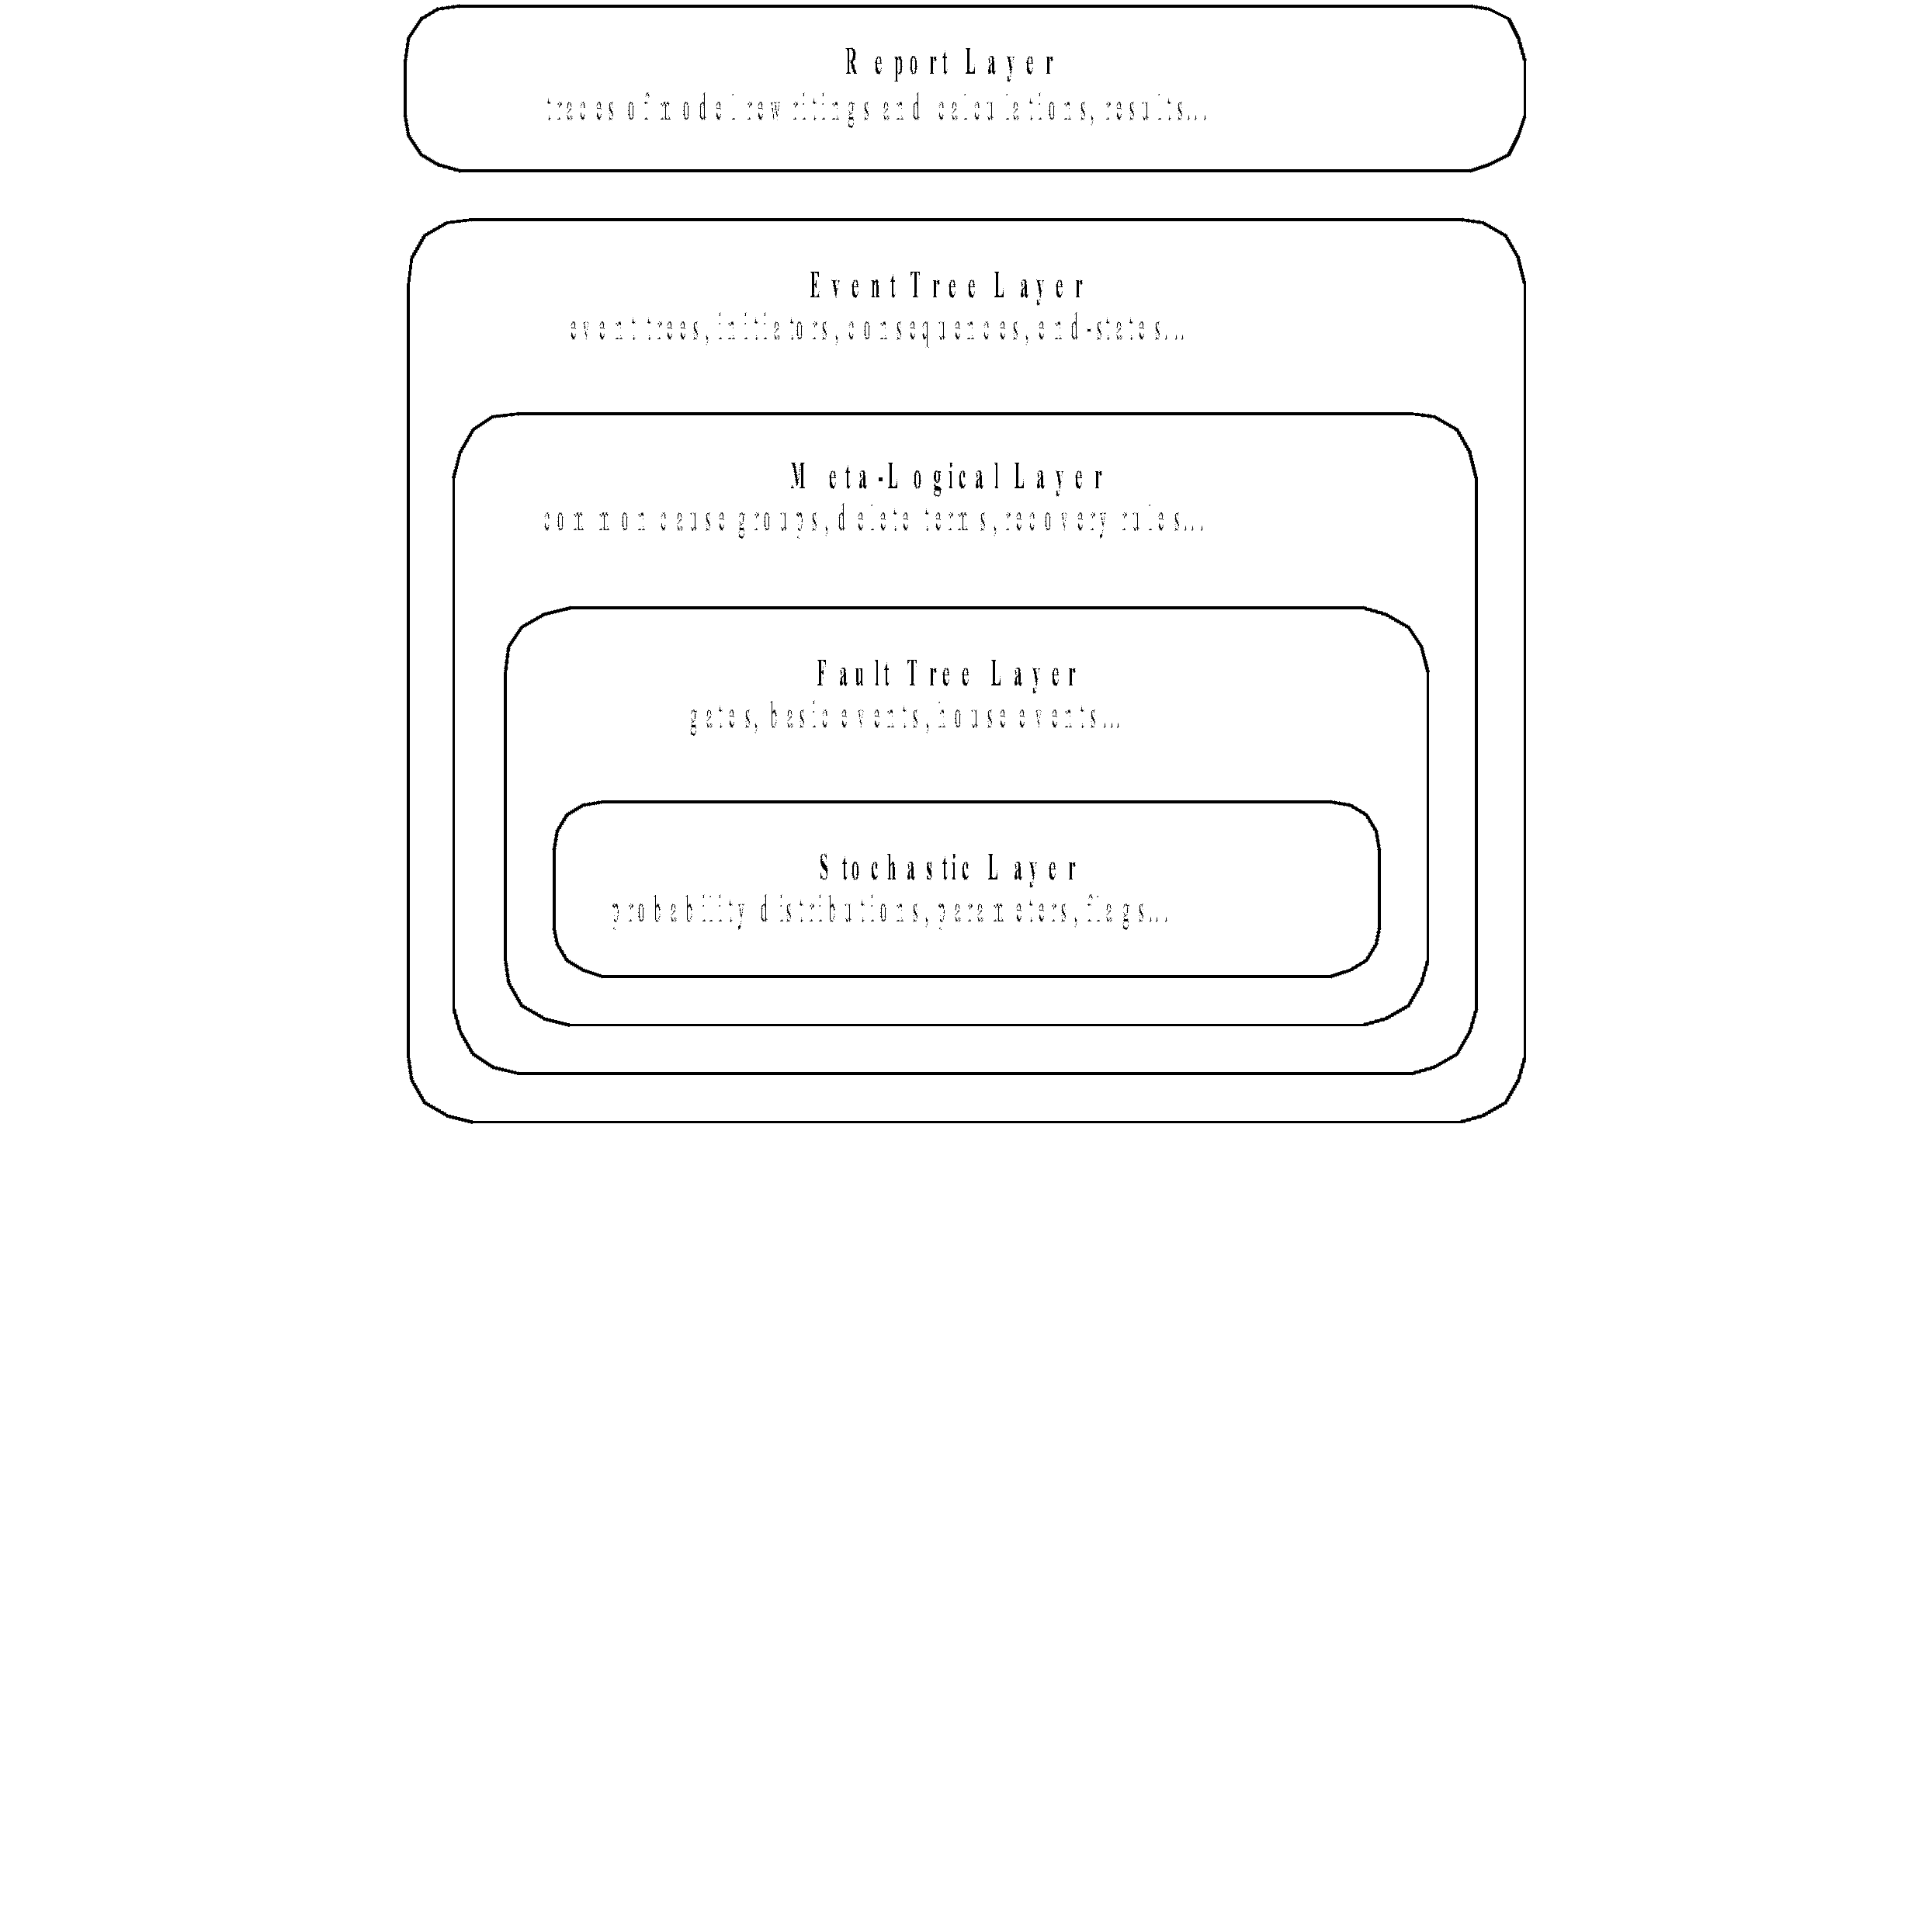
\includegraphics[width=0.9\textwidth]{./word/media/image3.png}
\caption{\label{fig:orgb04954f}
Architecture of the Model Exchange Format}
\end{figure}

\begin{itemize}
\item The first, or stochastic, layer is populated with all stochastic
aspects of models: probability distributions for the failure rates of
basic events, parameters of these distributions and distributions of
these parameters, flags\ldots{}

\item The second, or fault tree layer, is populated with logical components
of fault trees (gates, basic events, house events). This layer is the
core of PSA models. The two first layers can be used in isolation.
Some existing tools implement them only.

\item The third, or meta-logical, layer is populated constructs like common
cause groups, delete terms, recovery rules that are used to give
flavors to fault trees\ldots{}

\item The fourth, or event tree, layer is populated with event trees,
initiating events and consequences. The Model Exchange Format sees
event trees as (graphical) programs. The execution of such a program
produces a set of sequences, i.e. a set (a disjunction) of Boolean
formulae. Probability distributions are also collected while walking
the event tree.

\item The fifth, or report layer, is populated with constructs to store
results of calculations. This includes constructs to describe
calculations (version of the model, used engine, used cutoffs,
targeted group of consequences, calculated quantities\ldots{}) and well as
minimal cutsets and other results.
\end{itemize}

This five layers architecture helps to understand what the different
elements of a model are and what their respective roles are. In a word,
it is the backbone of the Model Exchange Format. It should be clear
however that any model will contain elements of the first fourth levels
and that these elements may be not arranged by levels. For instance, a
fault tree description will probably contain probability distributions
of basic events as well as common cause groups. Again, the five layers
architecture intends to differentiate elements according to their
meanings and operational behaviors.

\subsection{Formalism}
\label{sec:org6a3b3b4}

Throughout this document, we shall present a number of syntactic
constructions such as Boolean formulae, probability distributions, and
so on. These constructions will be eventually represented by means of
XML terms. XML is however a bit too verbose to make clear the underlying
mathematical nature of objects at hand. Therefore we shall use (in a
rather loose way) the Extended Backus-Naur form to define constructs. A
presentation of the Extended Backus-Naur form can be found in Appendix A..

There are several formal ways to describe a XML grammar. The most
popular one is probably the XML Document Type Definition (DTD). A DTD is
associated with an XML document via a Document Type Declaration, which
is a tag that appears near the start of the XML document. The
declaration establishes that the document is an instance of the type
defined by the referenced DTD. DTD are a good verification tools, but
hard to interpret by a human. Therefore, we shall present the grammar of
the Model Exchange Format mainly by means of examples and semi-formal
descriptions with the Extended Backus Naur form. A formal DTD for the
whole Model Exchange Format is given Appendix B.. A semi-formal
Backus-Naur form for the Model Exchange Format is given Appendix C..

It is worth noting that the XML descriptions we are giving here can be
extended in any way to fulfill the needs of a particular tool. In
particular, comments and pointers to documentation should be added here
and there to the model.

\subsection{Organization of the document}
\label{sec:org9729f86}

The remainder of this document is organized into six chapters
corresponding to an introductive overview, one chapter per layer of the
architecture of the Model Exchange Format and one additional chapter for
models as a whole.

\begin{itemize}
\item Chapter III gives an overview of main elements of a model and shows
how these elements are organized. It discusses how to split a
description into several files, how to solve naming conflicts\ldots{}

\item Chapter IV presents the fault tree layer. The fault tree layer is not
the lowest one in the hierarchy. However, fault trees are the most
basic and the central concept of PSA models. For this reason, we put
it in front.

\item Chapter V present the stochastic layer, i.e. all the mechanisms to
associate probability distributions to basic events.

\item Chapter VI presents the meta-logical layer.

\item Chapter VII presents the event tree layer.

\item Chapter VIII discusses the organization of models.

\item Finally, chapter presents the report/results layer, i.e. the
normalized format for results of assessment of PSA models.
\end{itemize}

Three appendices give additional details or summarize the contents of
these six chapters.

\begin{itemize}
\item Appendix A. presents the Backus-Naur form we use throughout this
document to describe both the mathematical structure of the
constructs and their XML representation.

\item Appendix B. gives the Document Type Definition (DTD) of the full
Model Exchange Format.

\item Appendix C. gives the Backus-Naur form of the Model Exchange Format.
\end{itemize}

\section{Anatomy of the Model Exchange Format}
\label{sec:org18ca51f}

This chapter presents the anatomy of the Model Exchange Format, i.e. the
main components of a model and their relationships. We assume the reader
is familiar with the fault tree/event tree methodology.

\subsection{Elements of a model}
\label{sec:org81bf3fc}

\subsubsection{Variables, Terms and Containers}
\label{sec:orga26274d}

Elements of a model are, as expected, components of fault trees/event
trees, namely basic events, gates, house events, probability
distributions, initiating events, safety systems, consequences\ldots{}
Conceptually, it is convenient to arrange most of these elements into
one of the three categories: terms, variables and containers.

\emph{Variables:} Variables are named elements. Gates, basic events, house
events, stochastic parameters, functional events, initiating events and
consequences are all variables. A variable is always defined, i.e.
associated with a term.

\emph{Terms:} Terms are built over variables, constants and operators. For
instance, the Boolean formula ``primary-motor-failure or
no-current-to-motor'' is a term built over the basic event
``primary-motor-failure'', the gate ``no-current-to-motor'' and the Boolean
operator ``or''. Similarly, the probability distribution
``1-exp(-lambda*t)'' is a term built over the numerical constant ``1'', the
failure rate ``lambda'' the time ``t'', and the three arithmetic operators
``-``, ``exp'' and ``*'' (``lambda'' and ``t'' are variables). Note that variables
are terms

\emph{Containers:} According to our terminology, a model is nothing but a set
of definitions of variables. Since a brute list of such definitions
would lack of structure, the Model Exchange Format makes it possible to
group them into containers. Containers have names and can be themselves
grouped into higher level containers. For instance, a fault tree is a
container for definitions of gates, house-events, basic events and
parameters of probability distributions. Similarly, an event tree is a
container for definitions of initiating events, functional events,
sequences\ldots{}

We are now ready to list the main elements of a model. The exact content
and role of these different elements will be detailed in the subsequent
chapters.

\subsubsection{Stochastic Layer}
\label{sec:org0dffb55}

\emph{Stochastic variables and terms:} Stochastic expressions are terms that
are used to define probability distributions (associated with basic
events). Stochastic variables are called parameters. For instance,
``1-exp(-lambda*t)'' is a stochastic expression built over the two
parameters ``lambda'' and ``t''.

From a programming viewpoint, it is convenient to group definitions of
parameters into (stochastic) containers. The stochastic layer is
populated with stochastic parameters, expressions and containers.

\subsubsection{Fault Tree Layer}
\label{sec:org702cd92}

\emph{Boolean formulae, Basic Events, House Events and Gates:} Boolean
formulae, or formulae for short, are terms built over the usual set of
constants (true, false), connectives (and, or, not\ldots{}) and Boolean
variables, i.e. Basic Events, Gates and House Events. Boolean variables
are called events, for that's what they represent in the sense of the
probability theory. Basic events are associated with probability
distributions, i.e. with (stochastic) expressions. Gates are defined as
Boolean formulae. House events are special gates that are defined as
Boolean constants only.

\emph{Fault Trees:} According to what precedes, a fault tree is container for
definitions of parameters, basic events, house events and gates.

The fault tree layer is populated with all elements we have seen so far.

\subsubsection{Meta-Logical Layer}
\label{sec:org6559b96}

The meta-logical layer contains extra-logical constructs in addition to
fault trees. These extra-logical constructs are used to handle issues
that are not easy to handle in a purely declarative and logical way.

\emph{Common Cause Groups:} Common cause groups are sets of basic events that
are not statistically independent. Several models can be used to
interpret common cause groups. All these models consist in splitting
each event of the group into a disjunction of independent basic events.

\emph{Substitutions:} delete terms, exchange events, and recovery rules are
global and extra-logical constraints that are used to describe
situations such as physical impossibilities, technical specifications,
or to modify the probability of a scenario according to some physical
rules or judgments about human actions. In the Model Exchange Format,
these extra-logical constructs are all modeled by means of the generic
notion of substitution.

\subsubsection{Event Tree Layer}
\label{sec:orgb8be0e6}

As we shall see, event trees must be seen as a (semi-)graphical language
to describe and to combine sequences. Elements of this language are the
following.

\emph{Event Trees:} Event Trees define scenarios from an Initiating Event (or
an Initiating Event Group) to different end-states. In the Model
Exchange Format, end-states are called Sequences. The same event tree
can be used for different Initiating Events. Along the scenarios,
``flavored'' copies of fault trees are collected and/or values are
computed. Flavors are obtained by changing values of house events and
parameters while walking along the tree. Event Trees are containers
according to our terminology. They contain definition of functional
events and states.

\emph{Initiating Events, Initiating Event Groups:}  Initiating Events describe
the starting point of an accidental sequence. They are always associated
with an event tree, although they are in general declared outside of
this event tree. The Model Exchange Format makes it possible to chain
event trees. Therefore, the end-state of a sequence of an event tree may
be the initiating event of another event tree. Initiating Events are
variables, according to our terminology. Initiating event groups are
sets of initiating events. Despite of their set nature, initiative
events are also variables, because an initiating event group may contain
another one (the initiating terms are set operations).

\emph{Functional Events:} Functional Events describe actions that are taken
to prevent an accident or to mitigate its consequences (usually by means
of a fault tree). Depending on the result of such an action, the
functional event may be in different, e.g. ``success'' or ``failure''.
Functional Events label the columns the graphical representation of
Event Trees.

\emph{Sequences, Branches:} Sequences are end-states of branches of event
trees. Branches are named intermediate states.

\emph{Instructions, Rules:} Instructions are used to describe the different
paths of an event tree, to set the states of functional events, to give
flavors of fault trees that are collected, and to communicate with the
calculation engine. Rules are (named) groups of Instructions. They
generalize split-fractions of the event tree linking approach, and
boundary condition sets of the fault tree linking approach.

\emph{Consequences, Consequence groups:} Consequences are couples made of an
initiating event and a sequence (an event tree end-state). Consequences
are named and are defined. They are variables according to our
terminology. Like Initiating Events, Consequences can be grouped to
study a particular type of accident. Consequence Groups are also
variables (the consequence terms are set operations).

\emph{Missions, Phases:} In some cases, the mission of the system is split
into different phase. The Model Exchange Format provides constructs to
reflect this situation.

\subsection{Structure of a model}
\label{sec:org75063f9}



\subsubsection{Relationships between elements of a model}
\label{sec:org1f7f69d}

The elements of a model, their layer and their dependencies are pictured
are pictured Figure \ref{im-main-el}. This schema illustrates the description
given in the previous section. Term categories are represented by
rectangles. Variables categories are represented by rounded rectangles.
A variable category is always included in a term category (for variables
are terms). The three container categories, namely models, event trees
and fault trees are represented by dashed rectangles. Dependencies among
categories are represented by arrows.

\begin{figure}[htbp]

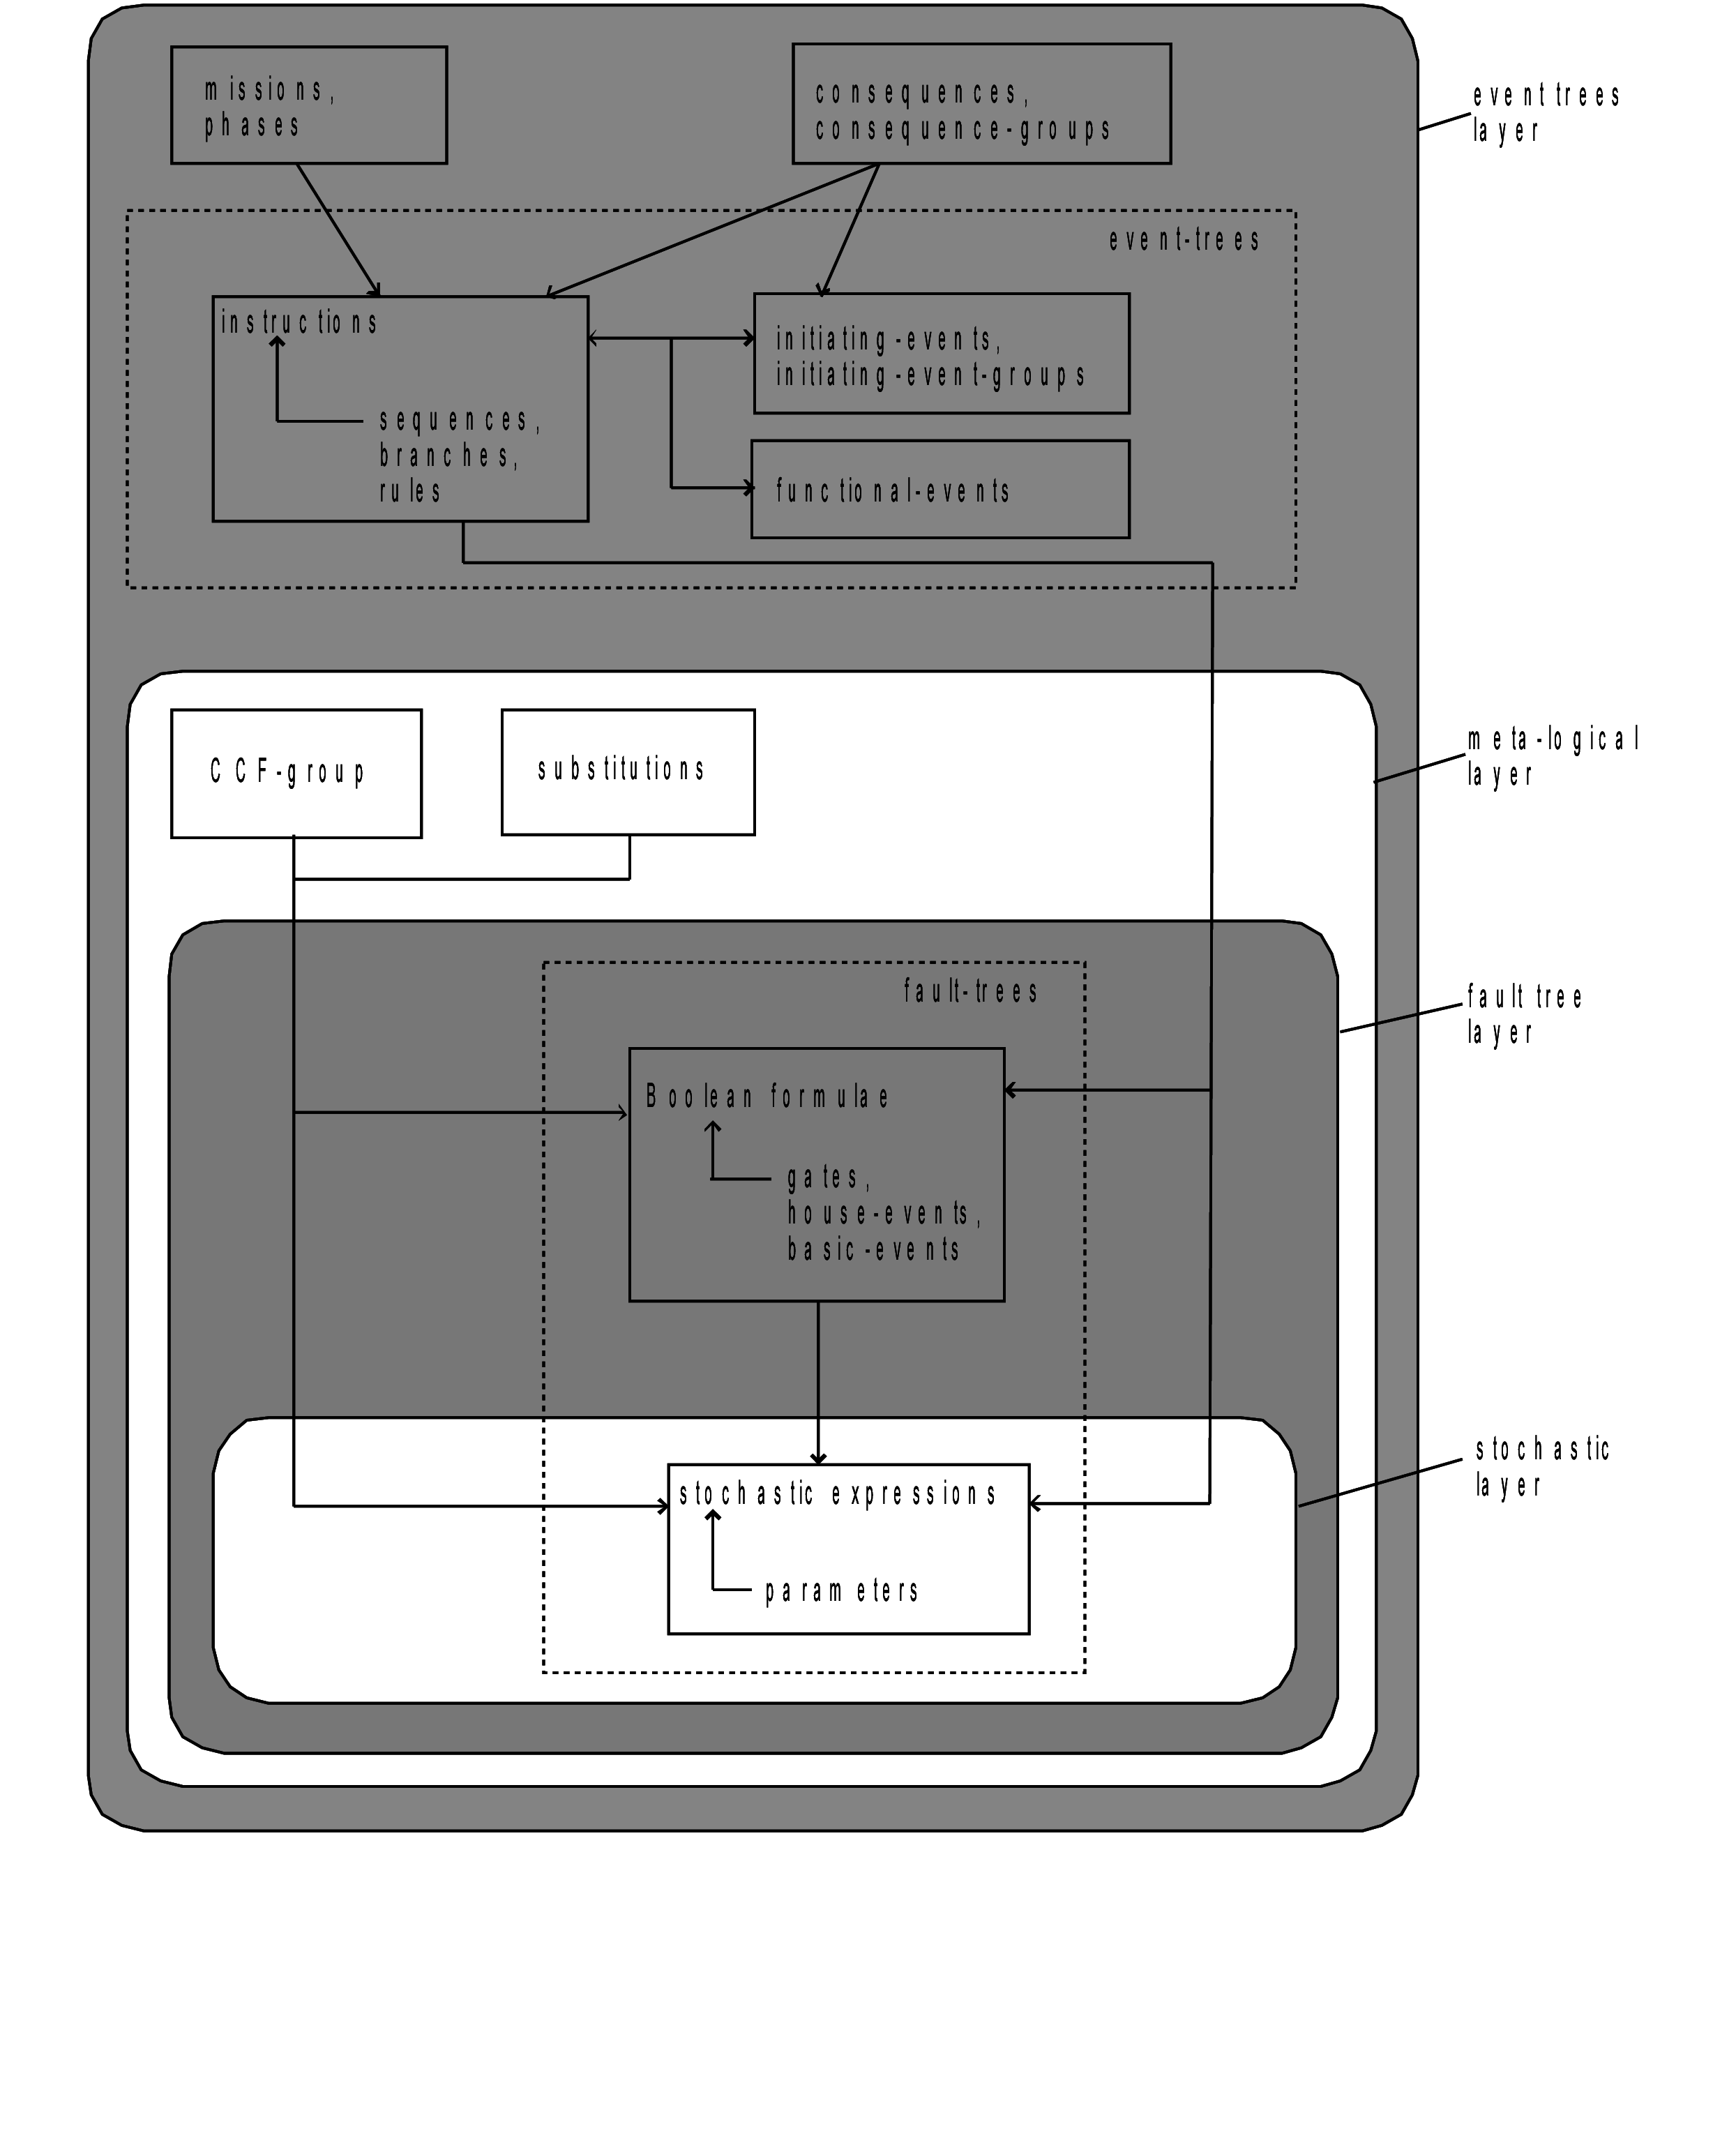
\includegraphics[width=0.9\textwidth]{./word/media/image4.png}
\caption{\label{fig:org6865508}
The main elements of a model, their layers and their dependencies}
\end{figure}

\subsubsection{Giving more structure to a model}
\label{sec:orgdee7e83}

A model (like a fault tree or an event tree) is a list of declarations.
The Model Exchange Format does not require structuring these
declarations: they can be given in any order, provided that the type of
an object can be decided prior to any use of this object. Fault trees
and event trees provide a first mean to organize models. This may be not
sufficient, especially when models are big. In order to structure
models, the Model Exchange Format provides the analyst with two
mechanisms.

First, declarations can be grouped together by means of user defined
containers. Such a container is just a XML tag. It has no semantics for
the model. It just makes it possible to delimit a set of objects of the
model that are physically or functionally related (for instance, the
different failure modes of a physical component).

Second, the Model Exchange Format makes it possible to associate user
defined attributes to the main components. For instance, we may define
an attribute ``zone'' with a value ``room33'' for all constructs describing
components located in the room 33. This indirect mean is very powerful.
It can be used extensively to perform calculations or changes on a
particular subset of elements.

\subsubsection{Containers as name spaces}
\label{sec:org84fd28c}

Once declared, elements are visible and accessible everywhere in the
model. This visibility means in turn that an object of a given type,
e.g. parameter or event, is unique. No two distinct objects of the same
type can have the same name. This constraint seems to be fine and
coherent. However, some tools do not obey the rule: two gates of two
different fault trees and representing two different functions may have
the same name. It is not possible to reject this possibility (as a bad
modeling practice), because when models are large and several persons
are working in collaboration, such name conflicts are virtually
impossible to avoid.

To solve this problem, the Model Exchange Format considers containers,
i.e. not only fault trees and event trees but also user defined
containers, as name spaces. By default, objects defined in a container
are global. But it is possible to declare them as local to the container
as well. In that case, they are not visible outside the container, and
tools are in charge of solving potential name conflicts.

\subsubsection{Definitions, Labels and Attributes}
\label{sec:org5f473ee}

Here follows some additional useful elements about the Model Exchange
Format.

\emph{Definitions versus references:} For the sake of the clarity (and for
XML specific reasons), it is important to distinguish the
declaration/definition of an element from references to that element.
For instance, we have to distinguish the definition of the gate
``motor-fails-to-start'' (as the Boolean formula ``primary-motor-failure or
no-current-to-motor''), from references to that gate into definitions of
other gates.

In the Model Exchange Format, the definition of a variable or a
container, for instance a gate, is in the following form.

\lstset{language=XML,label= ,caption= ,captionpos=b,numbers=none}
\begin{lstlisting}
<define-gate name="motor-fails-to-start" ...>
  ...
</define-gate>
\end{lstlisting}

References to that gate are in the following form.


\lstset{language=XML,label= ,caption= ,captionpos=b,numbers=none}
\begin{lstlisting}
...

<gate name="motor-fails-to-start" />

...
\end{lstlisting}

So, there are two tags for each element (variable or container) of the
Model Exchange Format: the tag ``define-element'' to define this element
and the tag ``element'' to refer this element. Note that the attribute
``name'' is systematically used to name elements.

\emph{Labels:} It is often convenient to add a comment to the definition of
an object. The Model Exchange Format defines a special tag ``label'' to do
so. The tag label can contain any text. It must be inserted as the first
child of the definition of the object. E.g.

\lstset{language=XML,label= ,caption= ,captionpos=b,numbers=none}
\begin{lstlisting}
<define-gate name="motor-fails-to-start" ...>
<label>
Warning: secondary motor failures are not taken into account here.
</label>
...
</define-gate>
\end{lstlisting}

\emph{Attributes:} Attributes can be associated with each element (variable
or container) of the Model Exchange Format. An attribute is a pair
(name, value), where both name and value are normally short strings.
Values are usually scalars, i.e. they are not interpreted. In order to
allow tools to interpret values, a third field ``type'' can be optionally
added to attributes. The tags ``attributes'' and ``attribute'' are used to
set attributes. The former is mandatory, even when only one attribute is
defined. It must be inserted as the first child of the definition of the
object, or just after the tag label, if any. E.g.
\lstset{language=XML,label= ,caption= ,captionpos=b,numbers=none}
\begin{lstlisting}
<define-gate name="motor-fails-to-start" ...>
<label>
Warning: secondary motor failures are not taken into account here.
</label>
<attributes>
<attribute name="zone" value="room33" />
...
</attributes>
...
</define-gate>
\end{lstlisting}

The Backus-Naur form for the XML representation of labels and attributes
is as follows.

\lstset{language=XML,label= ,caption= ,captionpos=b,numbers=none}
\begin{lstlisting}
label := <label> any text </label>
attributes ::= <attributes> attribute + </attributes>
attribute ::= <attribute name="identifier" value="string" [type="string" ] />
\end{lstlisting}

\section{Fault Tree Layer}
\label{sec:org5420222}

The Fault Tree layer is populated with logical components of Fault
Trees. It includes the stochastic layer, which contains itself the
probabilistic data. The stochastic layer will be presented in the next
section.

\subsection{Description}
\label{sec:orgd4a28b9}

Constituents of fault trees are Boolean variables (gates, basic events,
and house events), Boolean constants (true and false) and connectives
(and, or, k-out-of-n, not \ldots{}). Despite of their name, fault trees have
in general a directed acyclic graph structure (and not a tree-like
structure), because variables can be referenced more than once. The
simplest way to describe a fault tree is to represent it as a set of
equations in the form ``variable = Boolean-formula''. Variables that show
up as left hand side of an equation are gates. Variables that show up
only in right hand side formulae are basic events. Finally, variables
that show up only as left hand side of an equation are top events. Such
a representation imposes two additional conditions: first, the set of
equations must contain no loop, i.e. that the Boolean formula at the
right hand side of an equation must not depend, even indirectly
(recursively), on the variable at the left hand side. Second, a variable
must not show up more than once at the left hand side of an equation,
i.e. gates must be uniquely defined. Figure \ref{im-ft}  shows a Fault Tree.
The corresponding set of equations is as follows.


\begin{verse}
\vspace*{1em}
TOP = G1 or G2\\
\vspace*{1em}
G1 = H1 and G3 and G4\\
\vspace*{1em}
G2 = not H1 and BE2 and G4\\
\vspace*{1em}
G3 = BE1 or BE3\\
\vspace*{1em}
G4 = BE3 or BE4\\
\vspace*{1em}
\end{verse}

On the figure, basic events are surrounded with a circle. Basic events
are in general associated with a probability distribution (see Chapter
V).

House events (surrounded by a house shape frame on the figure) are
represented as variables but are actually constants: when the tree is
evaluated house events are always interpreted by their value, which is
either true or false. By default, house events take the value false.
Negated house events (gates, basic events) are represented by adding a
small circle over their symbol.

A semi-formal description of constructs of Fault Trees is given under
the Backus-Naur form \ref{FigureIV-4}. This description allows loops (in the
sense defined above), multiple definitions and trees with multiple top
events. The presence of loops must be detected by a specific check
procedure. If a variable or a parameter is declared more than once,
tools should emit a warning and consider only the last definition as the
good one (the previous ones are just ignored). In some circumstances, it
is of interest to define several fault trees at once by means of a
unique set of declarations. Therefore the presence of multiple top
events should not be prevented. We shall see what parameters and
expressions are in the next chapter.

\begin{figure}[htbp]

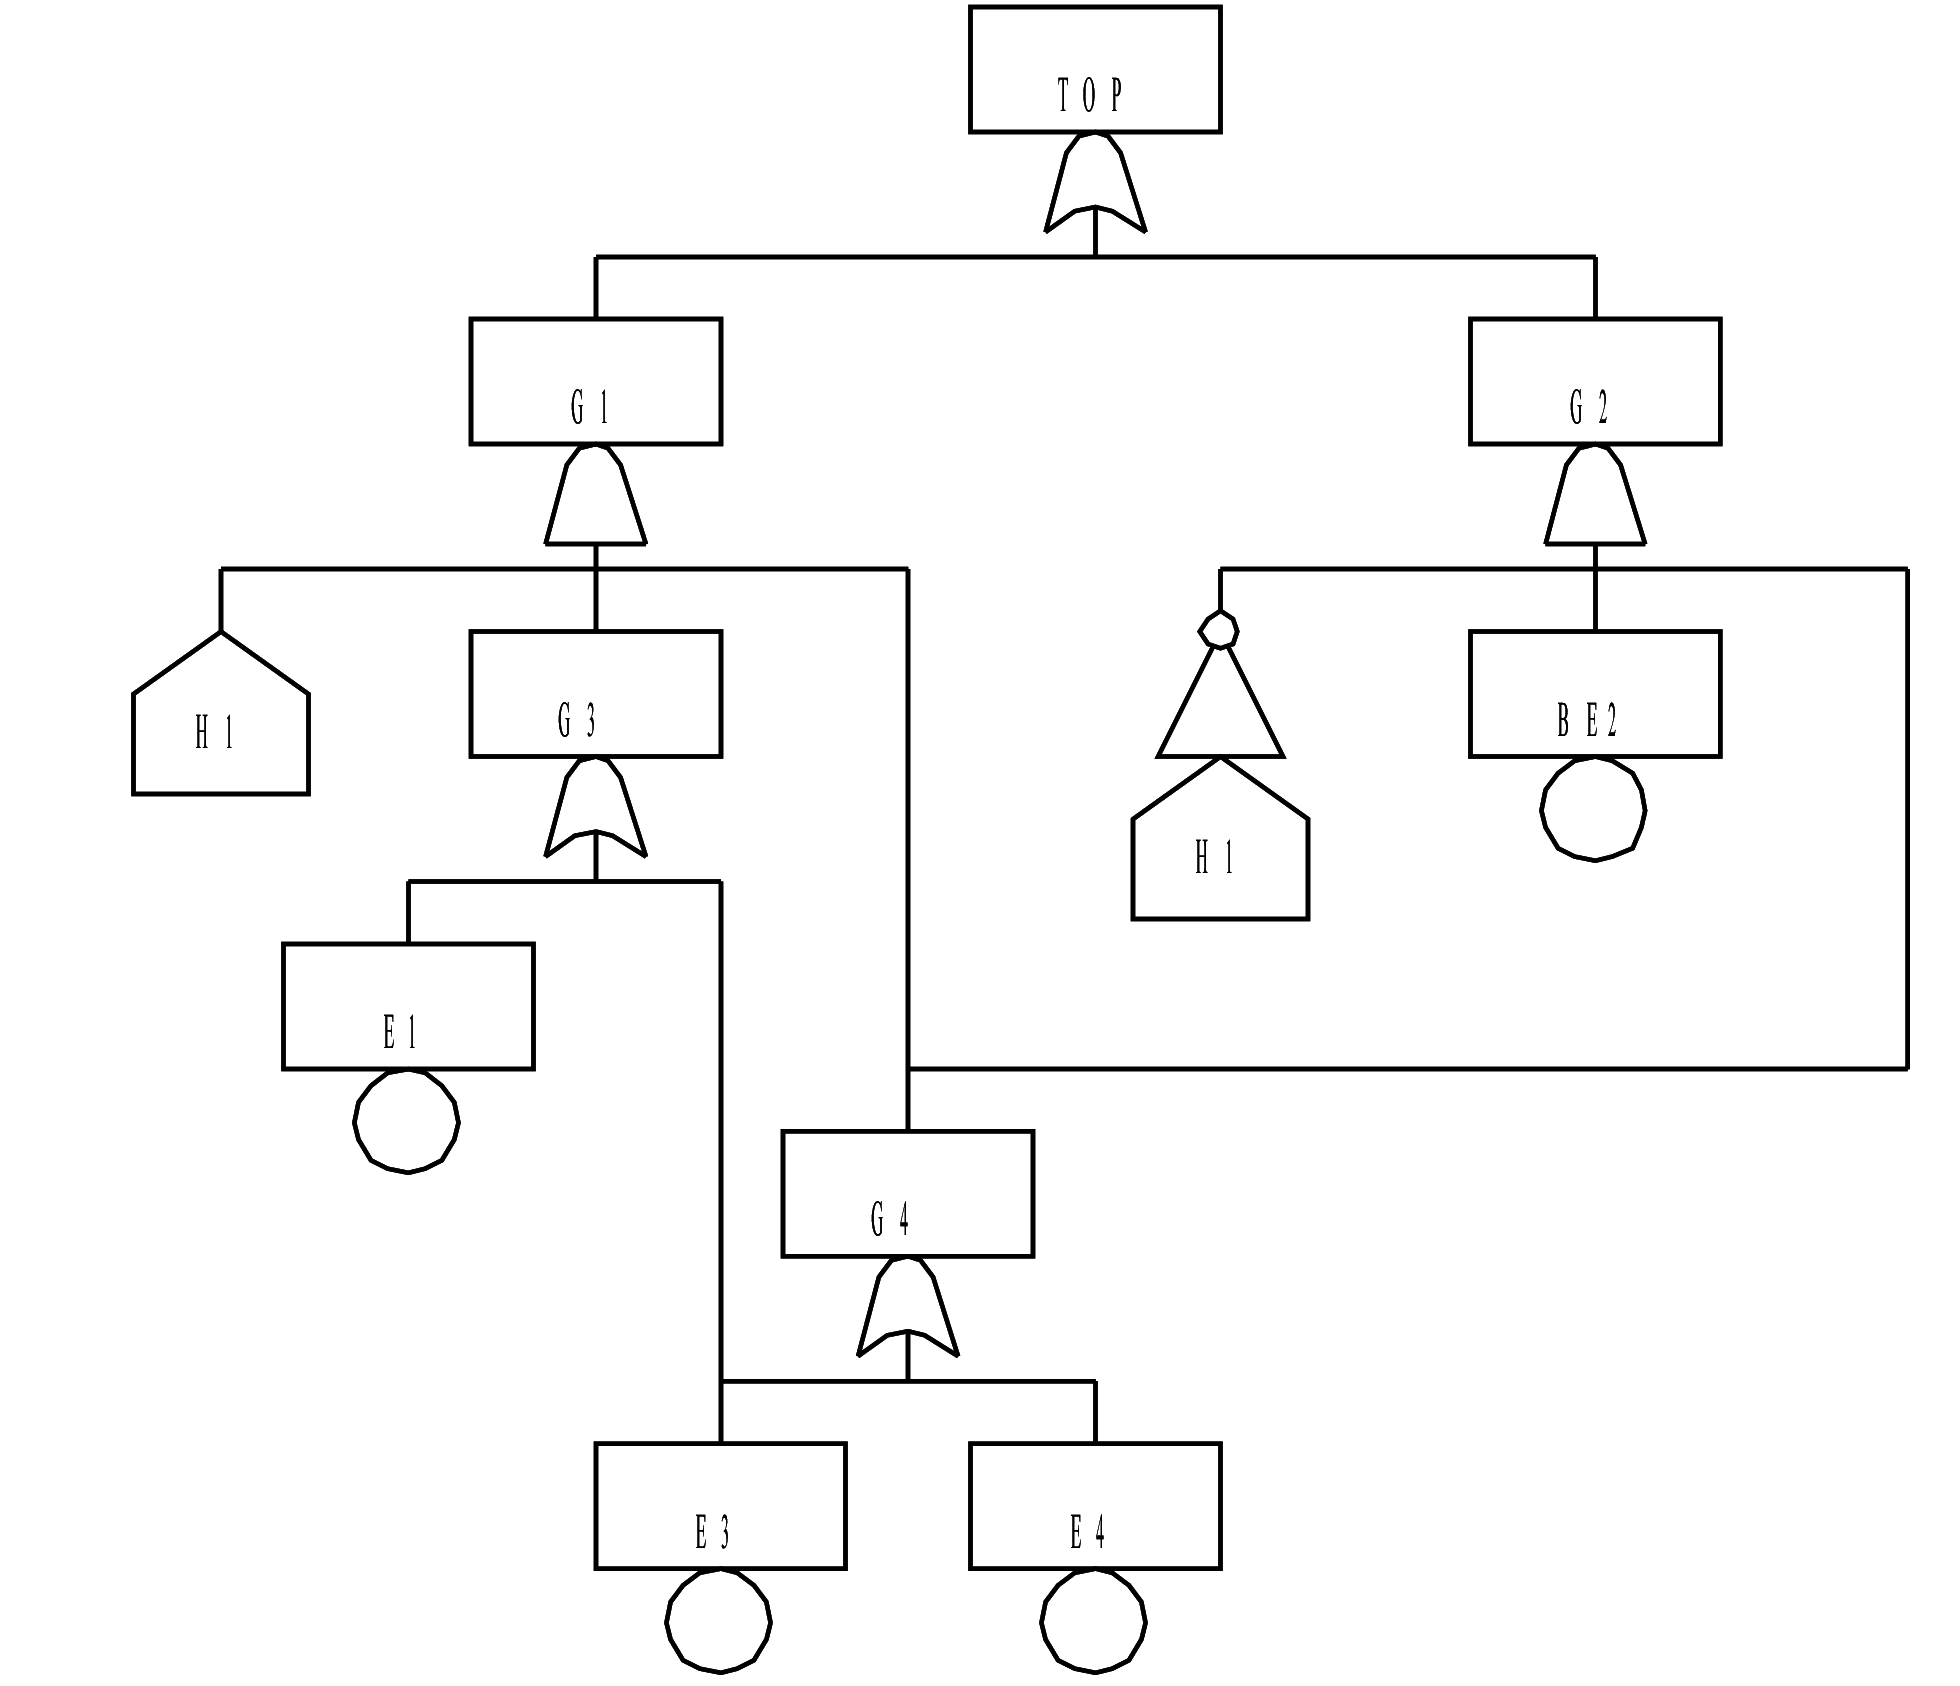
\includegraphics[width=0.9\textwidth]{./word/media/image5.png}
\caption{\label{fig:org66af9e4}
A Fault Tree}
\end{figure}

The semantics of connectives is given Table \ref{TableIV-1}. Note that connectives
``and'', ``or'', ``xor'', ``iff'', ``nand'' and ``nor'' are associative. Therefore
it suffices to give their semantics when they take two arguments, i.e.
two Boolean formulae F and G.


\lstset{language=XML,label= ,caption= ,captionpos=b,numbers=none}
\begin{lstlisting}
fault-tree-definition ::=
  fault-tree identifier ( event-definition | parameter-definition )

event-definition ::=

gate = formula
  | basic-event = expression
  | house-event = Boolean-constant

formula ::=
  event
  | Boolean-constant
  | and formula+
  | or formula+
  | not formula
  | xor formula+
  | iff formula+
  | nand formula+
  | nor formula+
  | atleast integer formula+
  | cardinality integer integer formula+
  | imply formula formula

event ::= gate | basic-event | house-event

Boolean-constant ::= constant (true | false)
\end{lstlisting}

\begin{table}[htbp]
\caption{\label{tab:org6263390}
Semantics of Boolean connectives}
\centering
\begin{tabular}{ll}
\textbf{Connective} & \textbf{Semantics}\\
\textbf{and} & F and G is true if both F and G are true, and false otherwise\\
\textbf{or} & F or G is true if either F or G is true, and false otherwise\\
\textbf{not} & not F is true if its F is false, and false otherwise\\
\textbf{xor} & F xor G is equivalent to (F and not G) or (not F and G)\\
\textbf{iff} & F iff G is equivalent to (F and G) or (not F and not G)\\
\textbf{nand} & F nand G is equivalent to not (F and G)\\
\textbf{nor} & F nor G is equivalent to not (F or G)\\
\textbf{atleast} & true if at least k out of the Boolean formulae given as arguments are true, and false otherwise. This connective is also called k-out-of-n, where k is the integer and n is the Boolean formulae given in arguments\\
\textbf{cardinality} & true if at least l and at most h of the Boolean formulae given as arguments are true, and false otherwise. l and h are the two integers (in order) given as arguments.\\
\textbf{imply} & F implies G is equivalent to not F and G\\
\end{tabular}
\end{table}




\begin{center}
\begin{tabular}{ll}
Dynamic Gates & In a second step, it would be of interest to incorporate to the Model Exchange Format ``inhibit'' gates, ``priority'' gates and ``triggers'' (like in Boolean Driven Markov processes). All of these dynamic gates can be interpreted as ``and'' gates in a Boolean framework. In more general frameworks (like Markovian frameworks) they can be interpreted in a different way, and provide mechanisms to model in an accurate way backup systems, limited amount of resources\ldots{} The complexity of the assessment of this kind of model is indeed much higher than the one of Boolean models (which is already at least NP-hard or \#P-hard).\\
\end{tabular}
\end{center}






\subsection{XML Representation}
\label{sec:orgf99aaba}

The Backus-Naur form for the XML description of fault trees is given
\ref{FigureIV-5} and \ref{FigureIV-6}.

This description deserves some comments.

\begin{itemize}
\item It leaves for now the tags ``define-parameter'' and ``expression''
unspecified. We shall see in the next chapter how these tags are used
to define the probability distributions.

\item Similarly, the tag ``define-component'' will be explained in the next
section.

\item Although the Model Exchange Format adopts the declarative modeling
paradigm, it is often convenient to use variables in formulae before
declaring them. The Model Exchange Format therefore refers to
variables with the generic term ``event'', possibly without a ``type''
attribute.

\item By default, the value of a house is event is ``false''. So it is not
necessary to associate a value with a house event when declaring it.
We shall see section VII.3 how to change the value of a house event.

\item Although events are typed (they are either gates, house events or
basic events), two different events cannot have the same name (within
the same name space), even if they are of different types. This point
will be explained in the next section.
\end{itemize}

\lstset{language=[LaTeX]TeX,label= ,caption= ,captionpos=b,numbers=none}
\begin{lstlisting}
fault-tree-definition ::=
  <define-fault-tree name="identifier" >
  [ label ]
  [ attributes ]
  (event-definition | parameter-definition |component-definition )*
  </define-fault-tree >
component-definition ::=
 <define-component name="identifier" [ role="private|public" ] >
 [ label ]
 [ attributes ]
 ( event-definition | parameter-definition | component-definition)*
  <define-component>
 model-data ::=
  <model-data>
     ( house-event-definition | basic-event-definition | parameter-definition )*
  </model-data>

event-definition ::=
   gate-definition
  | house-event-definition
  | basic-event-definition

gate-definition ::=
  <define-gate name="identifier" [ role="private|public" ] >
  [ label ]
  [ attributes ]
  formula
  </define-gate>

house-event-definition ::=
  <define-house-event name="identifier" [ role="private|public" ] >
  [ label ]
  [ attributes ]
  [ Boolean-constant ]
  </define-house-event>

basic-event-definition ::=
  <define-basic-event name="identifier" [ role="private|public" ] >
  [ label ]
  [ attributes ]
  [ expression ]
  </declare>
\end{lstlisting}

\lstset{language=[LaTeX]TeX,label= ,caption= ,captionpos=b,numbers=none}
\begin{lstlisting}
formula ::=
    event
  | Boolean-constant
  | <and> formula+ </and>
  | <or> formula+ </or>
  | <not> formula </not>
  | <xor> formula+ </xor>
  | <iff> formula+ </iff>
  | <nand> formula+ </nand>
  | <nor> formula+ </nor>
  | <atleast min="integer" > formula+ </atleast>
  | <cardinality min="integer" max="integer" > formula+  </cardinality>
  | <imply> formula formula </imply>

event ::=
  <event name="identifier" [ type="event-type" ] />
  | <gate name="identifier" />
  | <house-event name="identifier" />
  | <basic-event name="identifier" />

event-type ::= gate | basic-event | house-event

Boolean-constant ::= <constant value="Boolean-value" />

Boolean-value ::= true | false
\end{lstlisting}

The attribute ``role'' is used to declare whether an element is public or
private, i.e. whether it can be referred by its name everywhere in the
model or only within its inner most container. This point will be
further explained in the next section. This attribute is optional for by
default all elements are public.

The fault tree pictured \ref{FigureIV-3} is described \ref{FigureIV-7}. In this
representation, the house event ``h1'' has by default the value ``true''.
Basic events are not declared for it is not necessary, so no probability
distributions they are not associated with a probability distribution.

\lstset{language=XML,label= ,caption={XML description of Fault Tree pictured \ref{FigureIV-3}. \label{FigureIV-7}.},captionpos=b,numbers=none}
\begin{lstlisting}
<?xml version="1.0" ?>
<!DOCTYPE opsa-mef>
<opsa-mef>
  <define-fault-tree name="FT1" >
    <define-gate name="top">
      <or>
	<gate name="g1" />
	<gate name="g2" />
      </or>
    </define-gate>
    <define-gate name="g1">
      <and>
	<house-event name="h1" />
	<gate name="g3"/>
	<gate name="g4"/>
      </and>
    </define-gate>
    <define-gate name="g2">
      <and>
	<not>
	  <house-event name="h1" />
	</not>
	<basic-event name="e2" />
	<gate name="g4" />
      </and>
    </define-gate>
    <define-gate name="g3">
      <or>
	<basic-event name="e1" />
	<basic-event name="e3" />
      </or>
    </define-gate>
    <define-gate name="g4">
      <or>
	<basic-event name="e3" />
	<basic-event name="e4" />
      </or>
    </define-gate>
    <define-house-event name="h1" >
      <constant value="true" />
    </define-house-event>
  </define-fault-tree>
  <opsa-mef>
\end{lstlisting}



\subsection{Extra Logical Constructs and Recommendations}
\label{sec:org919658d}


\subsubsection{Model-Data and Components}
\label{sec:org46ba0cc}

The Model Exchange Format provides a number of extra-logical constructs
to document and structure models. Labels and attributes are introduced
Section III.2.4. They can be associated with declared element in order
to document this element. Fault trees are a first mean to structure
models. A fault tree groups any number of declarations of gates, house
events, basic event and parameters.

It is sometimes convenient to group definitions of house events, basic
events and parameters outside fault trees. The Model Exchange Format
provides the container ``model-data'' to do so.

The Model Exchange Format makes it possible to group further
declarations through the notion of component. A component is just a
container for declarations of events and parameters. It has a name and
may contain other components. The use of components is illustrated by
the following example.

Figure \ref{FigureIV-8} shows a fault tree FT with three components A, B and C. The
component B is nested into the component A. The XML representation for
this Fault Tree is given Figure \ref{FigureIV-9}. With a little anticipation, we
declared basic events. Note that components and fault trees may also
contain definitions of parameters. Note also that the basic event BE1,
which is declared in the component A, is used outside of this component
(namely in the sibling component C).


\begin{figure}[htbp]

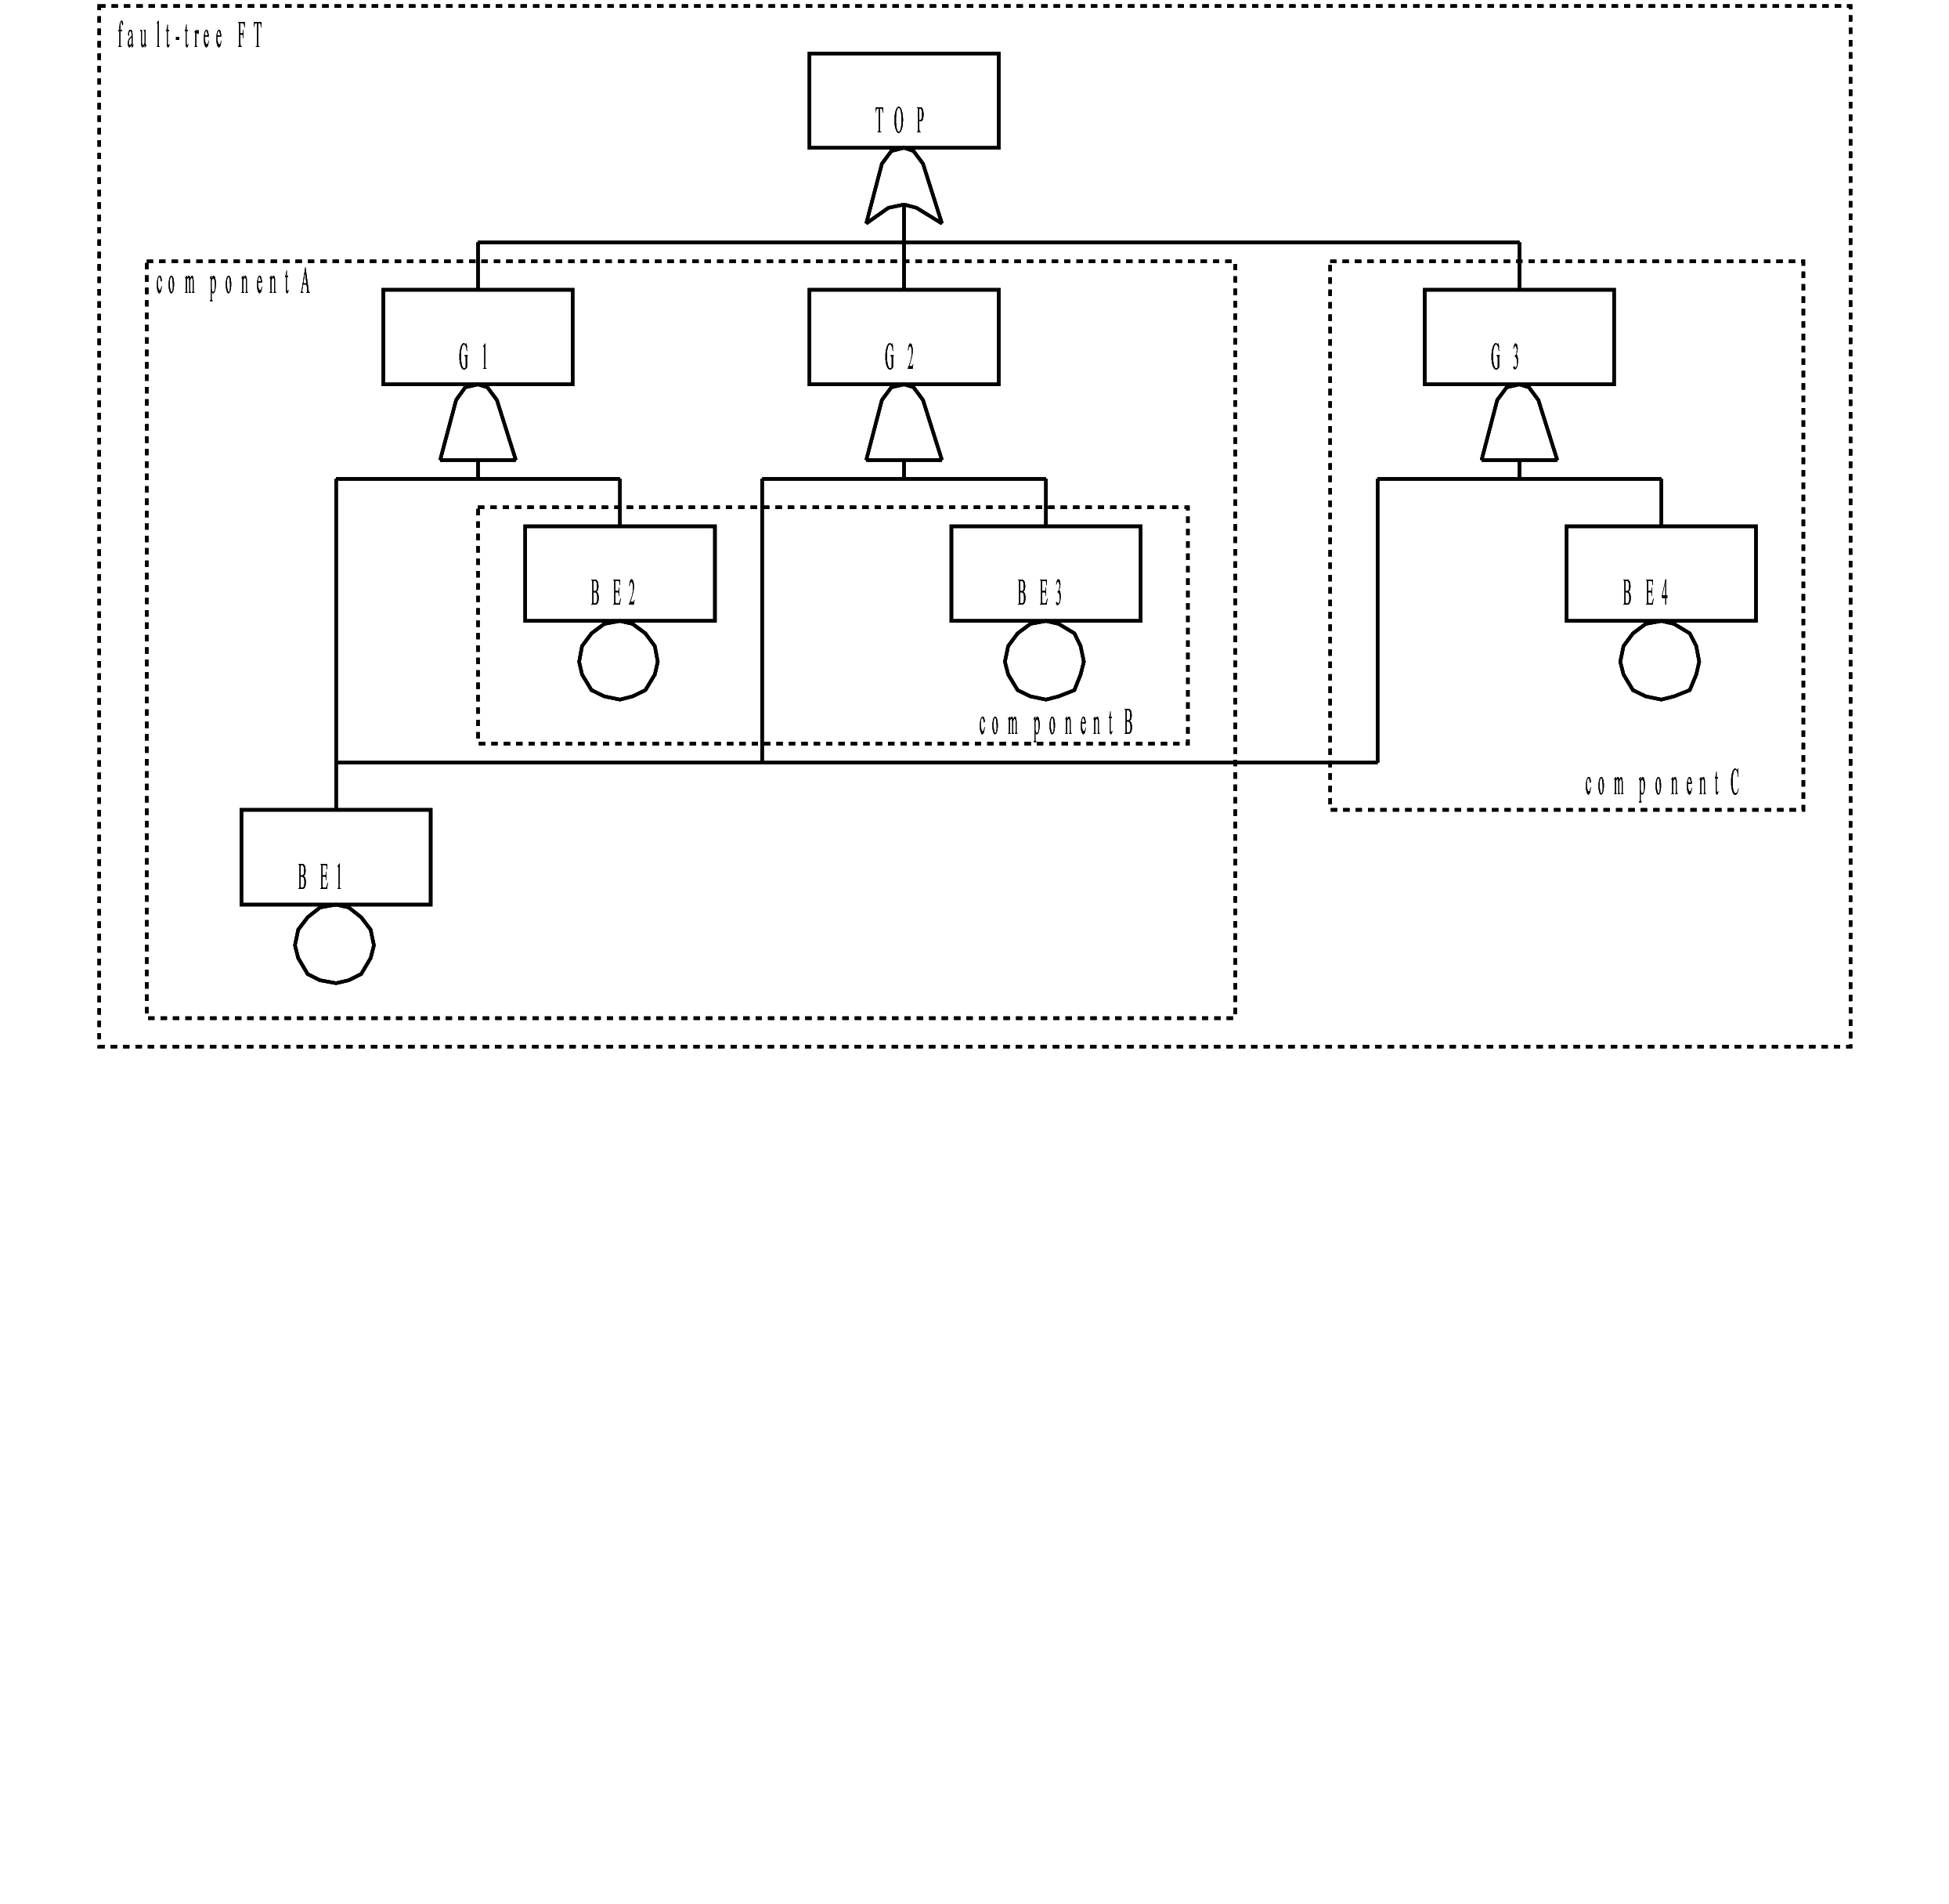
\includegraphics[width=0.9\textwidth]{./word/media/image6.png}
\caption{\label{fig:orga02dc11}
A Fault Tree with Three Components}
\end{figure}

\lstset{language=XML,label= ,caption={XML Representation for the Fault Tree pictured \ref{FigureIV-8}. \label{FigureIV-9}},captionpos=b,numbers=none}
\begin{lstlisting}
<define-fault-tree name="FT">
  <define-gate name="TOP">
    <or>
      <gate name="G1" />
      <gate name="G2" />
      <gate name="G3" />
    </or>
  </define-gate>
  <define-component name="A">
    <define-gate name="G1">
      <and>
	<basic-event name="BE1" />
	<basic-event name="BE2" />
      </and>
    </define-gate>
    <define-gate name="G2">
      <and>
	<basic-event name="BE1" />
	<basic-event name="BE3" />
      </and>
    </define-gate>
    <define-basic-event name="BE1" >
      <float value="1.2e-3" />
    </define-basic-event>
    <define-component name="B">
      <define-basic-event name="BE2" >
	<float value="2.4e-3" />
      </define-basic-event>
      <define-basic-event name="BE3" >
	<float value="5.2e-3" />
      </define-basic-event>
    </define-component>
  </define-component>
  <define-component name="C">
    <define-gate name="G3">
      <and>
	<basic-event name="BE1" />
	<basic-event name="BE4" />
      </and>
    </define-gate>
    <define-basic-event name="BE4" >
      <float value="1.6e-3" />
    </define-basic-event>
  </define-component>
</define-fault-tree>
\end{lstlisting}




\subsubsection{Solving Name Conflicts: Public versus Private Elements}
\label{sec:org52f3ce3}

By default, all of the elements of a model are public: they are visible
everywhere in the model and they can be referred by their name. For
instance, the basic event ``BE1'' of the fault tree pictured Figure \ref{FigureIV-9}
can be just referred as ``BE1''. This principle is fairly simple. It may
cause however some problem for large models, developed by several
persons: it is hard to prevent the same name to be used twice,
especially for what concerns gates (some software allow actually this
possibility).

The Model Exchange Format makes it possible to declare elements of fault
trees either as public or as private (to their inner most container).
Unless declared otherwise, an element is public if its innermost
container is public and private otherwise. For instance, if the
component ``A'' of the fault tree pictured Figure \ref{FigureIV-9} is declared as
private, then the component ``B'' (and its two basic events ``BE2'' and
``BE3''), the gates ``G1'' and ``G2'' and the basic event ``BE1'' are private by
default. There is no difference between public and private elements
except that two private elements of two different containers may have
the same name, while public elements must be uniquely defined.

There is actually three ways to refer an element:

\begin{itemize}
\item An element can be referred by its name. This works either if the
element is public or if it is referred inside the container (fault
tree or component) in which it is declared. For instance, if the
basic event ``BE1'' is public, it can be referred as ``BE1'' anywhere in
the model. If it is private, it can be referred as ``BE1'' only inside
the component ``A''.

\item An element can be referred by its full path (of containers), whether
it is public or private. The names of containers should be separated
with dots. For instance, the basic event ``BE2'' can be referred as
``FT.A.B.BE2'' anywhere in the model.

\item Finally, an element can be referred by its local path, whether it is
public or private. For instance, if the gate ``G1'' can be referred as
``FT.A.G1'' outside of the fault tree ``FT'', as ``A.G1'' inside the
declaration of ``FT'', and finally as ``G1'' inside the declaration of
the component ``A''. If the basic event BE1 is private (for a reason or
another), it should be referred either as ``FT.A.BE1'' inside the
component ``C''. In this case, the definition of the gate ``G3'' is as
follows.
\end{itemize}
\lstset{language=XML,label= ,caption= ,captionpos=b,numbers=none}
\begin{lstlisting}
<define-gate name="G3">
  <and>
    <basic-event name="FT.A.BE1" />
    <basic-event name="BE4" />
  </and>
</define-gate>
\end{lstlisting}

The important point here is that it is possible to name two private
elements of two different containers with the same identifier. For
instance, if components ``B'' and ``C'' are private, it is possible to
rename the basic-event ``BE4'' as ``BE2''. Outside these two components the
two basic events ``B2'' must be referred using their (local or global)
paths.

\subsubsection{Inherited attributes}
\label{sec:orgd4696d8}

Attributes associated with a container (fault tree, event tree or
component) are automatically inherited by all the elements declared in
the container. It is indeed possible to change the value of the
attribute at element level.

\subsubsection{Recommendations}
\label{sec:orgae35188}

\emph{Layered Models:} In PSA models, fault trees are in general layered,
i.e. arguments of connectives (and, or\ldots{}) are always either variables
or negations of variables. Although there is no reason to force such a
condition, it is recommended to obey it, for the sake of clarity.

\emph{Use Portable Identifiers:} In the XML description of fault trees, we
intentionally did not define identifiers. In many fault tree tools,
identifiers can be any string. It is however strongly recommended for
portability issues to use non problematic identifiers, like those of
programming languages, and to add a description of elements as a
comment. This means not using lexical entities such as spaces,
tabulations, ``.'' or ``/'' in names of elements, as well as realizing that
some old tools cannot differentiate between capital and small letters.

\emph{Role of Parameters, House Events and Basic Events:} Parameters, house
events and basic events should be always public, in order to facilitate
their portability from one tool to another.

\section{Stochastic Layer}
\label{sec:orgf2bd65d}

\subsection{Description}
\label{sec:orgb184d78}

The stochastic layer is populated with failure probabilities or failure
probability distributions associated with basic events (in the event
tree linking approach, functional events also can be associated with
such a distribution). Probability distributions are described by
(stochastic) expressions, which are terms, according to the terminology
of Chapter III. These expressions may depend on parameters (variables),
so the stochastic layer can be seen a set of stochastic equations.

Stochastic equations associated with basic events play actually two
roles:

\begin{itemize}
\item They are used to calculate probability distributions of each basic
event, i.e. for a given mission time t, the probability Q(t) that the
given basic event occurs before t. The probability distribution
associated with a basic event is typically a negative exponential
distribution of parameter \(\lambda\):
\end{itemize}

\begin{quote}
Note that, for the sake of the clarity, the Model Exchange Format
represents explicitly the mission time as a parameter of a special
type.
\end{quote}

\begin{itemize}
\item Parameters are sometimes not known with certainty. Sensitivity
analyses, such as Monte-Carlo simulations, are thus performed to
study the change in risk due to this uncertainty. Expressions are
therefore used to describe distributions of parameters. Typically,
the parameter \(\lambda\) of a negative exponential distribution will be itself
distributed according to a lognormal law of mean 0.001 and error
factor 3.
\end{itemize}

Stochastic expressions are made of the following elements:

\begin{itemize}
\item Boolean and numerical constants,

\item Stochastic variables, i.e. parameters, including the special variable
to represent the mission time,

\item Boolean and arithmetic operations (sums, differences, products\ldots{}),

\item Built-in expressions that can be seen as macro-expressions that are
used to simplify and shorten the writing of probability distributions
(E.g. exponential, Weibull\ldots{}),

\item Primitives to generate numbers at pseudo-random according to some
probability distribution. The base primitive makes it possible to
generate random deviates with a uniform probability distribution.
Several other primitives are derived from this one to generate random
deviates with normal, lognormal\ldots{} distributions. Moreover, it is
possible to define discrete distributions ``by hand'' through the
notion of histogram.

\item Directives to test the status of initial and functional events.
\end{itemize}

Figure V -10 sketches the Backus-Naur form for the constructs of the
stochastic layer. Note that, conversely to variables (events) of the
Fault Tree layer, parameters have to be defined (there is no equivalent
to Basic Events).



\lstset{language=[LaTeX]TeX,label= ,caption= ,captionpos=b,numbers=none}
\begin{lstlisting}
basic-event-declaration ::= basic-event = expression
parameter-declaration ::= parameter = expression
expression ::=
    constant | parameter | operation | built-in | random-deviate | test-event
constant ::= bool | integer | float
parameter ::= regular-parameter | system-mission-time
operation ::=
   and expression+
  | or expression+
  | not expression
  | eq expression expression
  | df expression expression
  ...
  | neg expression
  | add expression+
  | sub expression+
  | mul expression+
  | div expression+
  | pow expression expression
  ...
  | if expression then expression else expression

built-in ::=
  exponential expression expression
  | Weibull expression expression expression expression
  ...

random-deviate ::=
  uniform-deviate expression expression
  | lognormal-deviate expression expression expression
  | histogram
  ...

test-event ::=
  test-initial-event name
  | test-functional-event name state
\end{lstlisting}

The XML representation of the stochastic layer just reflects these
different constructs.

\lstset{language=[LaTeX]TeX,label= ,caption={Backus-Naur grammar for XML representation of expressions \label{FigureV-11}.},captionpos=b,numbers=none}
\begin{lstlisting}
parameter-definition ::=
  <define-parameter name="identifier"
  [ role="private|public" ] [ unit="unit" ]>
  [ label ] [ attributes ]
  expression
  </define-parameter>

unit ::= bool | int | float | hours | hours-1 | years | years-1| demands | fit

expression ::=
 constant | parameter | operation | built-in | random-deviate | test-event

constant ::=
  <bool value="Boolean-value" >
  | <int value="integer" >
  | <float value="float" >

parameter ::=
  <parameter name="identifier" [ unit="unit" ] >
  | <system-mission-time [ unit="unit" ] >

operation ::=
  numerical-operation | Boolean-operation | conditional-operation
\end{lstlisting}

(main)

Operations, built-ins and random deviates will be described in the
following sections.

We believe that the formalism to define stochastic equations should be
as large and as open as possible for at least two reasons: first,
available tools already propose a large set of distributions; second
this is a easy and interesting way to widen the spectrum of PSA. The
Model Exchange Format proposes a panoply of Boolean and arithmetic
operators. More operations can be added on demand. A major step would be
to introduce some algorithmic concepts like loops and functions. At this
stage, it does seem useful to introduce such advanced concepts in the
Model Exchange Format.

\subsection{Operations}
\label{sec:org40437c1}

\subsubsection{Numerical Operation}
\label{sec:org9be4c87}

Table \ref{TableV-2} gives the list of arithmetic operators proposed by the Model
Exchange Format. Their XML representation is given Figure \ref{FigureV-12}.


\begin{table}[htbp]
\caption{Numerical Operations, their number of arguments and their semantics \label{TableV-2}}
\centering
\begin{tabular}{lrl}
\textbf{Operator} & \textbf{\#arguments} & \textbf{Semantics}\\
\textbf{neg} & 1 & unary minus\\
\textbf{add} & >1 & addition\\
\textbf{sub} & >1 & subtraction\\
\textbf{mul} & >1 & multiplication\\
\textbf{div} & >1 & division\\
\textbf{pi} & 0 & 3.1415926535\ldots{}\\
\textbf{abs} & 1 & absolute value\\
\textbf{acos} & 1 & arc cosine of the argument in radians\\
\textbf{asin} & 1 & arc sine of the argument in radians\\
\textbf{atan} & 1 & arc tangent of the argument in radians\\
\textbf{cos} & 1 & cosine\\
\textbf{cosh} & 1 & hyperbolic cosine\\
\textbf{exp} & 1 & exponential\\
\textbf{log} & 1 & (Neperian) logarithm\\
\textbf{log10} & 1 & decimal logarithm\\
\textbf{mod} & 2 & modulo\\
\textbf{pow} & 1 & power\\
\textbf{sin} & 1 & sine\\
\textbf{sinh} & 1 & hyperbolic sine\\
\textbf{tan} & 1 & tangent\\
\textbf{tanh} & 1 & hyperbolic tangent\\
\textbf{sqrt} & 1 & square root\\
\textbf{ceil} & 1 & first integer greater than the argument\\
\textbf{floor} & 1 & first integer smaller than the argument\\
\textbf{min} & >1 & minimum\\
\textbf{max} & >1 & maximum\\
\textbf{mean} & >1 & mean\\
\end{tabular}
\end{table}




\lstset{language=[LaTeX]TeX,label= ,caption= ,captionpos=b,numbers=none}
\begin{lstlisting}
numerical-operation ::=

   <neg> expression </neg>
| <add> expression+ </add>
| <sub> expression+ </sub>
| <mul> expression+ </mul>
| <div> expression+ </div>
| <pi />
| <abs> expression </abs>
| <acos> expression </acos>
| <asin> expression </asin>
| <atan> expression </atan>
| <cos> expression </cos>
| <cosh> expression </cosh>
| <exp> expression </exp>
| <log> expression </log>
| <log10> expression </log10>
| <mod> expression expression </mod>
| <pow> expression expression </pow>
| <sin> expression </sin>
| <sinh> expression </sinh>
| <tan> expression </tan>
| <tanh> expression </tanh>
| <sqrt> expression </sqrt>
| <ceil> expression </ceil>
| <floor> expression </floor>
| <min> expression+ </min>
| <max> expression+ </max>
| <mean> expression+ </mean>
\end{lstlisting}

\emph{Example}: Assume for instance we want to associate a negative
exponential distribution with a failure rate \(\lambda\)=1.23e-4/h to the basic
event ``pump-failure''. Using primitives defined above, we can encode
explicitly such probability distribution as follows.


\lstset{language=XML,label= ,caption= ,captionpos=b,numbers=none}
\begin{lstlisting}
<define-basic-event name="pump-failure" >
  <sub>
    <float value="1.0" />
    <exp>
      <mul>
	<neg>
	  <parameter name="lambda" />
	</neg>
	<system-mission-time />
      </mul>
    </exp>
  </sub>
</define-basic-event>
<define-parameter name="lambda" >
  <float value="1.23e-4" />
</define-parameter>
\end{lstlisting}


\subsubsection{Boolean Operations}
\label{sec:orgf31a61a}


Table V-3 gives the list of Boolean operators proposed by the Model
Exchange Format. Their XML representation is given Figure \ref{TableV-13}.

\begin{table}[htbp]
\caption{Boolean operators, their number of arguments and their semantics \label{TableV-3}.}
\centering
\begin{tabular}{lrl}
\textbf{Operator} & \textbf{\#arguments} & \textbf{Semantics}\\
\textbf{and} & > 1 & Boolean and\\
\textbf{or} & >1 & Boolean or\\
\textbf{not} & 1 & Boolean not\\
\textbf{eq} & 2 & =\\
\textbf{df} & 2 & \(\neq\)\\
\textbf{lt} & 2 & <\\
\textbf{gt} & 2 & >\\
\textbf{leq} & 2 & \(\le\)\\
\textbf{geq} & 2 & \(\ge\)\\
\end{tabular}
\end{table}


\lstset{language=[LaTeX]TeX,label= ,caption={Backus-Naur grammar for XML representation of Boolean operations \label{FigureV-13}.},captionpos=b,numbers=none}
\begin{lstlisting}
Boolean-operation ::=
<not> expression </not>
  | <and> expression+ </and>
  | <or> expression+ </or>
  | <eq> expression expression </eq>
  | <df> expression expression </df>
  | <lt> expression expression </lt>
  | <gt> expression expression </gt>
  | <leq> expression expression </leq>
  | <geq> expression expression </geq>
\end{lstlisting}



\subsubsection{Conditional Operations}
\label{sec:org7fd4c8c}

The Model Exchange Format proposes two conditional operations: an
``if-then-else'' operation and a ``switch/case'' operation. The latter is a
list of pairs of expressions, introduced by the tag ``case''. The first
expression of the pair should be a Boolean condition. If this condition
is realized, then the second expression is evaluated and its value
returned. Otherwise, the next pair is considered.

The list ends with an expression, in order to be sure that the switch
has always a possible value. The XML representation for conditional
operation is given Figure \ref{FigureV-14}.

\lstset{language=[LaTeX]TeX,label= ,caption={Backus-Naur grammar for XML representation of conditional operations \label{FigureV-14}.},captionpos=b,numbers=none}
\begin{lstlisting}
conditional-operation ::=
if-then-else-operation | switch-operation
if-then-else-operation ::=
<ite> expression expression expression <ite>
switch-operation ::=
<switch>
case-operation*
expression
<switch>
case-operation ::=
<case> expression expression <case>
\end{lstlisting}



\emph{Example:} Assume for instance we want to give different values to the
failure rate ``lambda'' depending on a global parameter ``stress-level":

\lstset{language=[LaTeX]TeX,label= ,caption= ,captionpos=b,numbers=none}
\begin{lstlisting}
``lambda''=1.0e-4/h if ``stress-level''=1,

``lambda''=2.5e-4/h if ``stress-level''=2, and finally

``lambda''=1.0e-3/h if ``stress-level''=3.
\end{lstlisting}

The value of ``stress-level''will be modified while walking along the
sequences of events trees or depending on the initiating event. Using
primitives defined so far, we can encode the definition of ``lambda'' as
follows.


\lstset{language=XML,label= ,caption= ,captionpos=b,numbers=none}
\begin{lstlisting}
<define-parameter name="lambda" >
  <switch>
    <case>
      <eq>
	<parameter name="stress-level" />
	<int value="1" />
      </eq>
      <float value="1.0e-4" />
    </case>
    <case>
      <eq>
	<parameter name="stress-level" />
	<int value="2" />
      </eq>
      <float value="2.5e-4" />
    </case>
    <float value="1.0e-3" />
  </switch>
</define-parameter>
\end{lstlisting}

\subsection{Built-Ins}
\label{sec:org6e86502}


\subsubsection{Description}
\label{sec:org44a926f}

Built-ins can be seen as macro arithmetic expressions. They are mainly
used to simplify the writing of probability distributions. A special
built-in ``extern-function'' makes it possible to define externally
calculated built-ins. As for arithmetic operators, more built-ins can be
added on demand to the Model Exchange Format. Here follows a preliminary
list of built-ins. Table IV -1 summarizes this preliminary list.

\emph{Exponential with two parameters:} this built-in implements the negative
exponential distribution. The two parameters are the hourly failure
rate, usually called \(\lambda\), and the time t. It definition is as follows.

\emph{Exponential with four parameters (GLM):} this built-in generalizes the
previous one. It makes it possible to take into account repairable
components (through the hourly repairing rate \emph{µ}) and failures on
demand (through the probability \(\gamma\) of such an event). It takes four
parameters, \(\gamma\), the hourly failure rate \(\lambda\), \emph{µ} and the time t (in this
order). Its definition is as follows.

\emph{Weibull:} this built-in implements the Weibull distribution. It takes
four parameters: a scale parameter \emph{\(\alpha\)}, a shape parameter \emph{\(\beta\)}, a time
shift t\(_{\text{0}}\), and the time t (in this order). Its definition is as
follows.

\emph{Periodic test:} In several applications, it is of interest to introduce
some specific distributions to describe periodically tested components.
A further investigation is certainly necessary on this topic. We
tentatively give here a candidate definition (that is extracted from one
of the tools we considered).

The ``periodic-test'' built-in would take the following parameters (in
order).

\begin{table}[htbp]
\caption{Table illustrates the meaning of the parameters \(\tau\), \(\theta\) and \(\pi\). \label{FigureV-15}}
\centering
\begin{tabular}{ll}
\(\lambda\) & failure rate when the component is working.\\
 & \\
\(\lambda\)* & failure rate when the component is tested.\\
 & \\
µ & repair rate (once the test showed that the component is failed).\\
 & \\
\(\tau\) & delay between two consecutive tests.\\
 & \\
\(\theta\) & delay before the first test.\\
 & \\
\(\gamma\) & probability of failure due to the (beginning of the) test.\\
 & \\
\(\pi\) & duration of the test.\\
 & \\
x & indicator of the component availability during the test (1 available, 0 unavailable).\\
 & \\
\(\sigma\) & test covering: probability that the test detects the failure, if any.\\
 & \\
\(\omega\) & probability that the component is badly restarted after a test or a repair.\\
 & \\
t & the mission time.\\
 & \\
\end{tabular}
\end{table}





\begin{figure}[htbp]

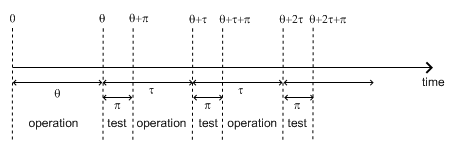
\includegraphics[width=0.9\textwidth]{./word/media/image7.png}
\caption{\label{fig:orgc941764}
Meaning of parameters \(\tau\), \(\theta\) and \(\pi\) of the ``periodic-test'' built-in.}
\end{figure}

There are three phases in the behaviour of the component. The first
phase corresponds to the time from 0 to the date of the first test, i.e.
\(\theta\). The second phase is the test phase. It spreads from times \(\theta\)+n.\(\tau\) to
\(\theta\)+n.\(\tau\)+\(\pi\), with n any positive integer. The third phase is the functioning
phase. It spreads from times \(\theta\)+n.\(\tau\)+\(\pi\) from \(\theta\)+(n+1).\(\tau\).

In the first phase, the distribution is a simple exponential law of
parameter \(\lambda\).

The component may enter in the second phase in three states, either
working, failed or in repair. In the latter case, the test is not
performed. The Markov graphs for each of these cases are pictured Figure \ref{im-Multi-phase}.


\begin{figure}[htbp]

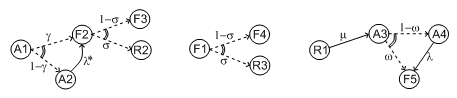
\includegraphics[width=0.9\textwidth]{./word/media/image8.png}
\caption{\label{fig:org842e743}
Multi-phase Markov graph for the ``periodic-test'' built-in.}
\end{figure}

Ai's , Fi's, Ri's states correspond respectively to states where the
component is available, failed and in repair. Dashed lines correspond to
immediate transitions. Initial states are respectively A1, F1 and R1.

The situation is simpler in the third phase. If the component enters
available this phase, the distribution follows an exponential law of
parameter \(\lambda\). If the component enters failed in this phase, it remains
phase up to the next test. Finally, the Markov graph for the case where
the component is in repair is the same as in the second phase.

The Model Exchange Format could provide also two simplified forms for
the periodic test distribution.

\emph{Periodic-test with 5 arguments:} The first one takes five parameters:
\(\lambda\), µ, \(\tau\), \(\theta\) and t. In that case, the test is assumed to be instantaneous.
Therefore, parameters \(\lambda\)* (the failure rate during the test) and x
(indicator of the component availability during the test) are
meaningless. There other parameters are set as follows.

\begin{itemize}
\item \(\gamma\) (the probability of failure due to the beginning of the test) is
set to 0.

\item \(\sigma\) (the probability that the test detects the failure, if any) is set
to 1.

\item \(\omega\) (the probability that the component is badly restarted after a test
or a repair) is set to 0.
\end{itemize}

\emph{Periodic-test with 4 arguments:}  The second one takes only four
parameters: \(\lambda\), \(\tau\), \(\theta\) and t. The repair is assumed to be instantaneous (or
equivalently the repair rate µ = +\(\infty\)).

\emph{Extern functions:} The Model Exchange Format should provide a mean to
call extern functions. This makes it extensible and allows the link the
PSA assessment tools with complex tools to calculate physical behavior
(like fire propagation or gas dispersion). This call may take any number
of arguments and return a single value at once (some interfacing glue
can be used to handle the case where several values have to be
returned). It has been also suggested that extern function calls take
XML terms as input and output. This is probably the best way to handle
communication between tools, but it would be far too complex too embed
XML into stochastic expressions.


\begin{table}[htbp]
\caption{Built-ins, their number of arguments and their semantics \label{TableV-4}}
\centering
\begin{tabular}{lrl}
\textbf{Built-in} & \textbf{\#arguments} & \textbf{Semantics}\\
\textbf{exponential} & 2 & negative exponential distribution with hourly failure rate and time\\
\textbf{exponential} & 4 & negative exponential distribution with probability of failure on demand, hourly failure rate, hourly repair rate and time\\
\textbf{Weibull} & 4 & Weibull distribution with scale and shape parameters, a time shift and the time\\
\textbf{periodic-test} & 11, 5 or 4 & Distributions to describe periodically tested components\\
\textbf{extern-function} & any & call to an extern routine\\
\end{tabular}
\end{table}

\subsubsection{XML Representation}
\label{sec:org9821d9f}

The Backus-Naur grammar for the XML representation of built-ins is given Figure \ref{FigureV-17}.


\lstset{language=[LaTeX]TeX,label= ,caption={Backus-Naur grammar for XML representation of Built-ins \label{FigureV-17}},captionpos=b,numbers=none}
\begin{lstlisting}
built-in ::=
   <exponential> [ expression ]:2 </exponential>
  | <GLM> [ expression ]:4 </GLM>
  | <Weibull> [ expression ]:3 </Weibull>
  | <periodic-test> [ expression ]:11 </periodic-test>
  | <periodic-test> [ expression ]:5 </periodic-test>
  | <periodic-test> [ expression ]:4 </periodic-test>
  | <extern-function name="name" > expression* </extern-function>
\end{lstlisting}

\begin{center}
\begin{tabular}{ll}
Positional & We adopted a positional definition of arguments. For instance, in the negative exponential distribution, we assumed that the failure rate is always the first argument and the mission time always the second. An alternative way would be to name arguments, i.e. to enclose them into tags explicating their role. For instance, the failure rate would be enclosed in a tag ``failure-rate'', the mission time in a tag ``time'' and so on\ldots{} The problem with this second approach is that many additional tags must be defined and it is not sure that it helps a lot the understanding of the built-ins. Nevertheless, we may switch to this approach if the experience shows that the first one proves to be confusing.\\
 & \\
versus & \\
 & \\
named & \\
 & \\
arguments & \\
\end{tabular}
\end{center}

\emph{Example:} The negative exponential distribution can be encoded in a
simple way as follows.


\lstset{language=XML,label= ,caption= ,captionpos=b,numbers=none}
\begin{lstlisting}
<define-basic-event name="pump-failure" >
    <exponential>
	 <parameter name="lambda" />
	 <system-mission-time />
	 </exponential>
</define-basic-event>
\end{lstlisting}


\subsection{Primitive to Generate Random Deviates}
\label{sec:orgc5833ee}


\subsubsection{Description}
\label{sec:org558cd25}

Primitives to generate random deviates are the real stochastic part of
stochastic equations. They can be used in two ways: in a regular context
they return a default value (typically their mean value). When used to
perform Monte-Carlo simulations, they return a number drawn at
pseudo-random according their type. The Model Exchange Format includes
two types of random deviates: built-in deviates like uniform, normal or
lognormal and histograms that are user defined discrete distributions. A
preliminary list of distributions which is summarized Table V -5. As for
arithmetic operators and built-ins, this list can be extended on demand.



\begin{center}
\begin{tabular}{lrl}
\textbf{Distribution} & \textbf{\#arguments} & \textbf{Semantics}\\
\textbf{uniform-deviate} & 2 & uniform distribution between a lower and an upper bounds\\
\textbf{normal-deviate} & 2 & normal (Gaussian) distribution defined by its mean and its standard deviation\\
\textbf{lognormal-deviate} & 3 & lognormal distribution defined by its mean, its error factor and the confidence level of this error factor\\
\textbf{gamma-deviate} & 2 & gamma distributions defined by a shape and a scale factors\\
\textbf{beta-deviate} & 2 & beta distributions defined by two shape parameters \(\alpha\) and \(\beta\)\\
\textbf{histograms} & any & discrete distributions defined by means of a list of pairs\\
\end{tabular}
\end{center}


\emph{Uniform Deviates:} These primitives describe uniform distributions in a
given range defined by its lower- and upper-bounds. The default value of
a uniform deviate is the mean of the range, i.e. (lower-bound +
upper-bound)/2.

\emph{Normal Deviates}: These primitives describe normal distributions
defined by their mean and their standard deviation (refer to text book
for a more detailed explanation). By default, the value of a normal
distribution is its mean.

\emph{Lognormal distribution:} These primitives describe lognormal
distributions defined by their mean µ and their error factor EF. A
random variable is distributed according to a lognormal distribution if
its logarithm is distributed according to a normal distribution. If µ
and \(\sigma\) are respectively the mean and the standard deviation of the
distribution, the probability density of the random variable is as
follows.

Its mean, \emph{E(x)} is defined as follows.

The confidence intervals \emph{[X\(_{\text{0,05}}\), X\(_{\text{0,95}}\)]} associated with a
confidence level of \emph{0.95} and the median \emph{X\(_{\text{0,50}}\)} are the following:

The error factor \emph{EF} is defined as follows:

with and .

Once the mean and the error factor are known, it is then possible to
determine the confidence interval and thereby the parameters of the
lognormal law.

\emph{Gamma Deviates:} These primitives describe Gamma distributions defined
by their shape parameter k and their scale parameter \(\theta\). If k is an
integer then the distribution represents the sum of k exponentially
distributed random variables, each of which has mean \(\theta\).

The probability density of the gamma distribution can be expressed in
terms of the gamma function:

The default value of the gamma distribution is its mean, i.e. k.\(\theta\).

\emph{Beta Deviates:} These primitives describe Beta distributions defined by
two shape parameters \(\alpha\) and \(\beta\).

The probability density of the beta distribution can be expressed in
terms of the B function:

The default value of the gamma distribution is its mean, i.e. \(\alpha\)/(\(\alpha\)+\(\beta\)).

\emph{Histograms:} Histograms are lists of pairs (x\(_{\text{1}}\), E\(_{\text{1}}\))\ldots{} (x\(_{\text{n}}\),
E\(_{\text{n}}\)) where the x\(_{\text{i}}\)'s are numbers such that x\(_{\text{i}}\) < x\(_{\text{i+1}}\) for
i=1\ldots{}n-1 and the E\(_{\text{i}}\)'s are expressions.

The x\(_{\text{i}}\)'s represent upper bounds of successive intervals. The lower
bound of the first interval x\(_{\text{0}}\) is given apart.

The drawing of a value according to a histogram is a two steps process.
First, a value z is drawn uniformly in the range [x\(_{\text{0}}\), x\(_{\text{n}}\)]. Then, a
value is drawn at random by means of the expression E\(_{\text{i}}\), where i is
the index of the interval such x\(_{\text{i-1}}\)< z \(\le\) x\(_{\text{i}}\).

By default, the value of a histogram is its mean, i.e.

Both Cumulative Distribution Functions and Density Probability
Distributions can be translated into histograms.

A Cumulative Distribution Function is a list of pairs (p\(_{\text{1}}\), v\(_{\text{1}}\))\ldots{}
(p\(_{\text{n}}\), v\(_{\text{n}}\)), where the p\(_{\text{i}}\)'s are such that p\(_{\text{i}}\) < p\(_{\text{i+1}}\) for
i=1\ldots{} n and p\(_{\text{n}}\)=1. It differs from histograms in two ways. First, X
axis values are normalized (to spread between 0 and 1) and second they
are presented in a cumulative way. The histogram that corresponds to a
Cumulative Distribution Function (p\(_{\text{1}}\), v\(_{\text{1}}\))\ldots{} (p\(_{\text{n}}\), v\(_{\text{n}}\)) is the
list of pairs (x\(_{\text{1}}\), v\(_{\text{1}}\))\ldots{} (x\(_{\text{n}}\), v\(_{\text{n}}\)), with the initial value
x\(_{\text{0}}\) is 0, x\(_{\text{1}}\) = p\(_{\text{1}}\) and x\(_{\text{i}}\) = p\(_{\text{i}}\) - p\(_{\text{i-1}}\) for all i>1.

A Discrete Probability Distribution is a list of pairs (d\(_{\text{1}}\), m\(_{\text{1}}\))\ldots{}
(d\(_{\text{n}}\), m\(_{\text{n}}\)). The d\(_{\text{i}}\)'s are probability densities. They could be
however any kind of values. The m\(_{\text{i}}\)'s are midpoints of intervals and
are such that m\(_{\text{1}}\) < m\(_{\text{2}}\) < \ldots{} < m\(_{\text{n}}\) < 1. The histogram that
corresponds to a Discrete Probability Distribution (d\(_{\text{1}}\), m\(_{\text{1}}\))\ldots{}
(d\(_{\text{n}}\), m\(_{\text{n}}\)) is the list of pairs (x\(_{\text{1}}\), d\(_{\text{1}}\))\ldots{} (x\(_{\text{n}}\), d\(_{\text{n}}\)),
with the initial value x\(_{\text{0}}\) = 0, x\(_{\text{1}}\) = 2.m\(_{\text{1}}\) and x\(_{\text{i}}\) = x\(_{\text{i-1}}\) +
2.(m\(_{\text{i}}\)-x\(_{\text{i-1}}\)).

\subsubsection{XML Representation}
\label{sec:orgb5abc78}

The Backus-Naur grammar for the XML representation of random deviates is
given


\lstset{language=[LaTeX]TeX,label= ,caption={\label{FigureV-18}. Backus-Naur grammar for XML representation of random deviates},captionpos=b,numbers=none}
\begin{lstlisting}
random-deviate ::=

  <uniform-deviate> [ expression ]:2 </uniform-deviate>
  | <normal-deviate> [ expression ]:2 </normal-deviate>
  | <lognormal-deviate> [ expression ]:3 </lognormal-deviate>
  | <gamma-deviate> [ expression ]:2 </gamma-deviate>
  | <beta-deviate> [ expression ]:2 </beta-deviate>
  | histogram

histogram ::=
  <histogram > expression /bin/+ </histogram>

/bin/ ::=
  <bin> expression expression </bin>
\end{lstlisting}


\emph{Example:} Assume that the parameter ``lambda'' of a negative exponential
distribution is distributed according to a lognormal distribution of
mean 0.001 and error factor 3 for a confidence level of 95\%. The
parameter ``lambda'' is then defined as follows.


\lstset{language=XML,label= ,caption= ,captionpos=b,numbers=none}
\begin{lstlisting}
<define-parameter name="lambda" >
<lognormal-deviate>
<float value="0.001" />
<float value="3" />
<float value="0.95" />
</lognormal-deviate>
</define-parameter>
\end{lstlisting}

\emph{Example:} Assume that the parameter ``lambda'' has been sampled outside
of the model and is distributed according to the following histogram.

\begin{figure}[htbp]

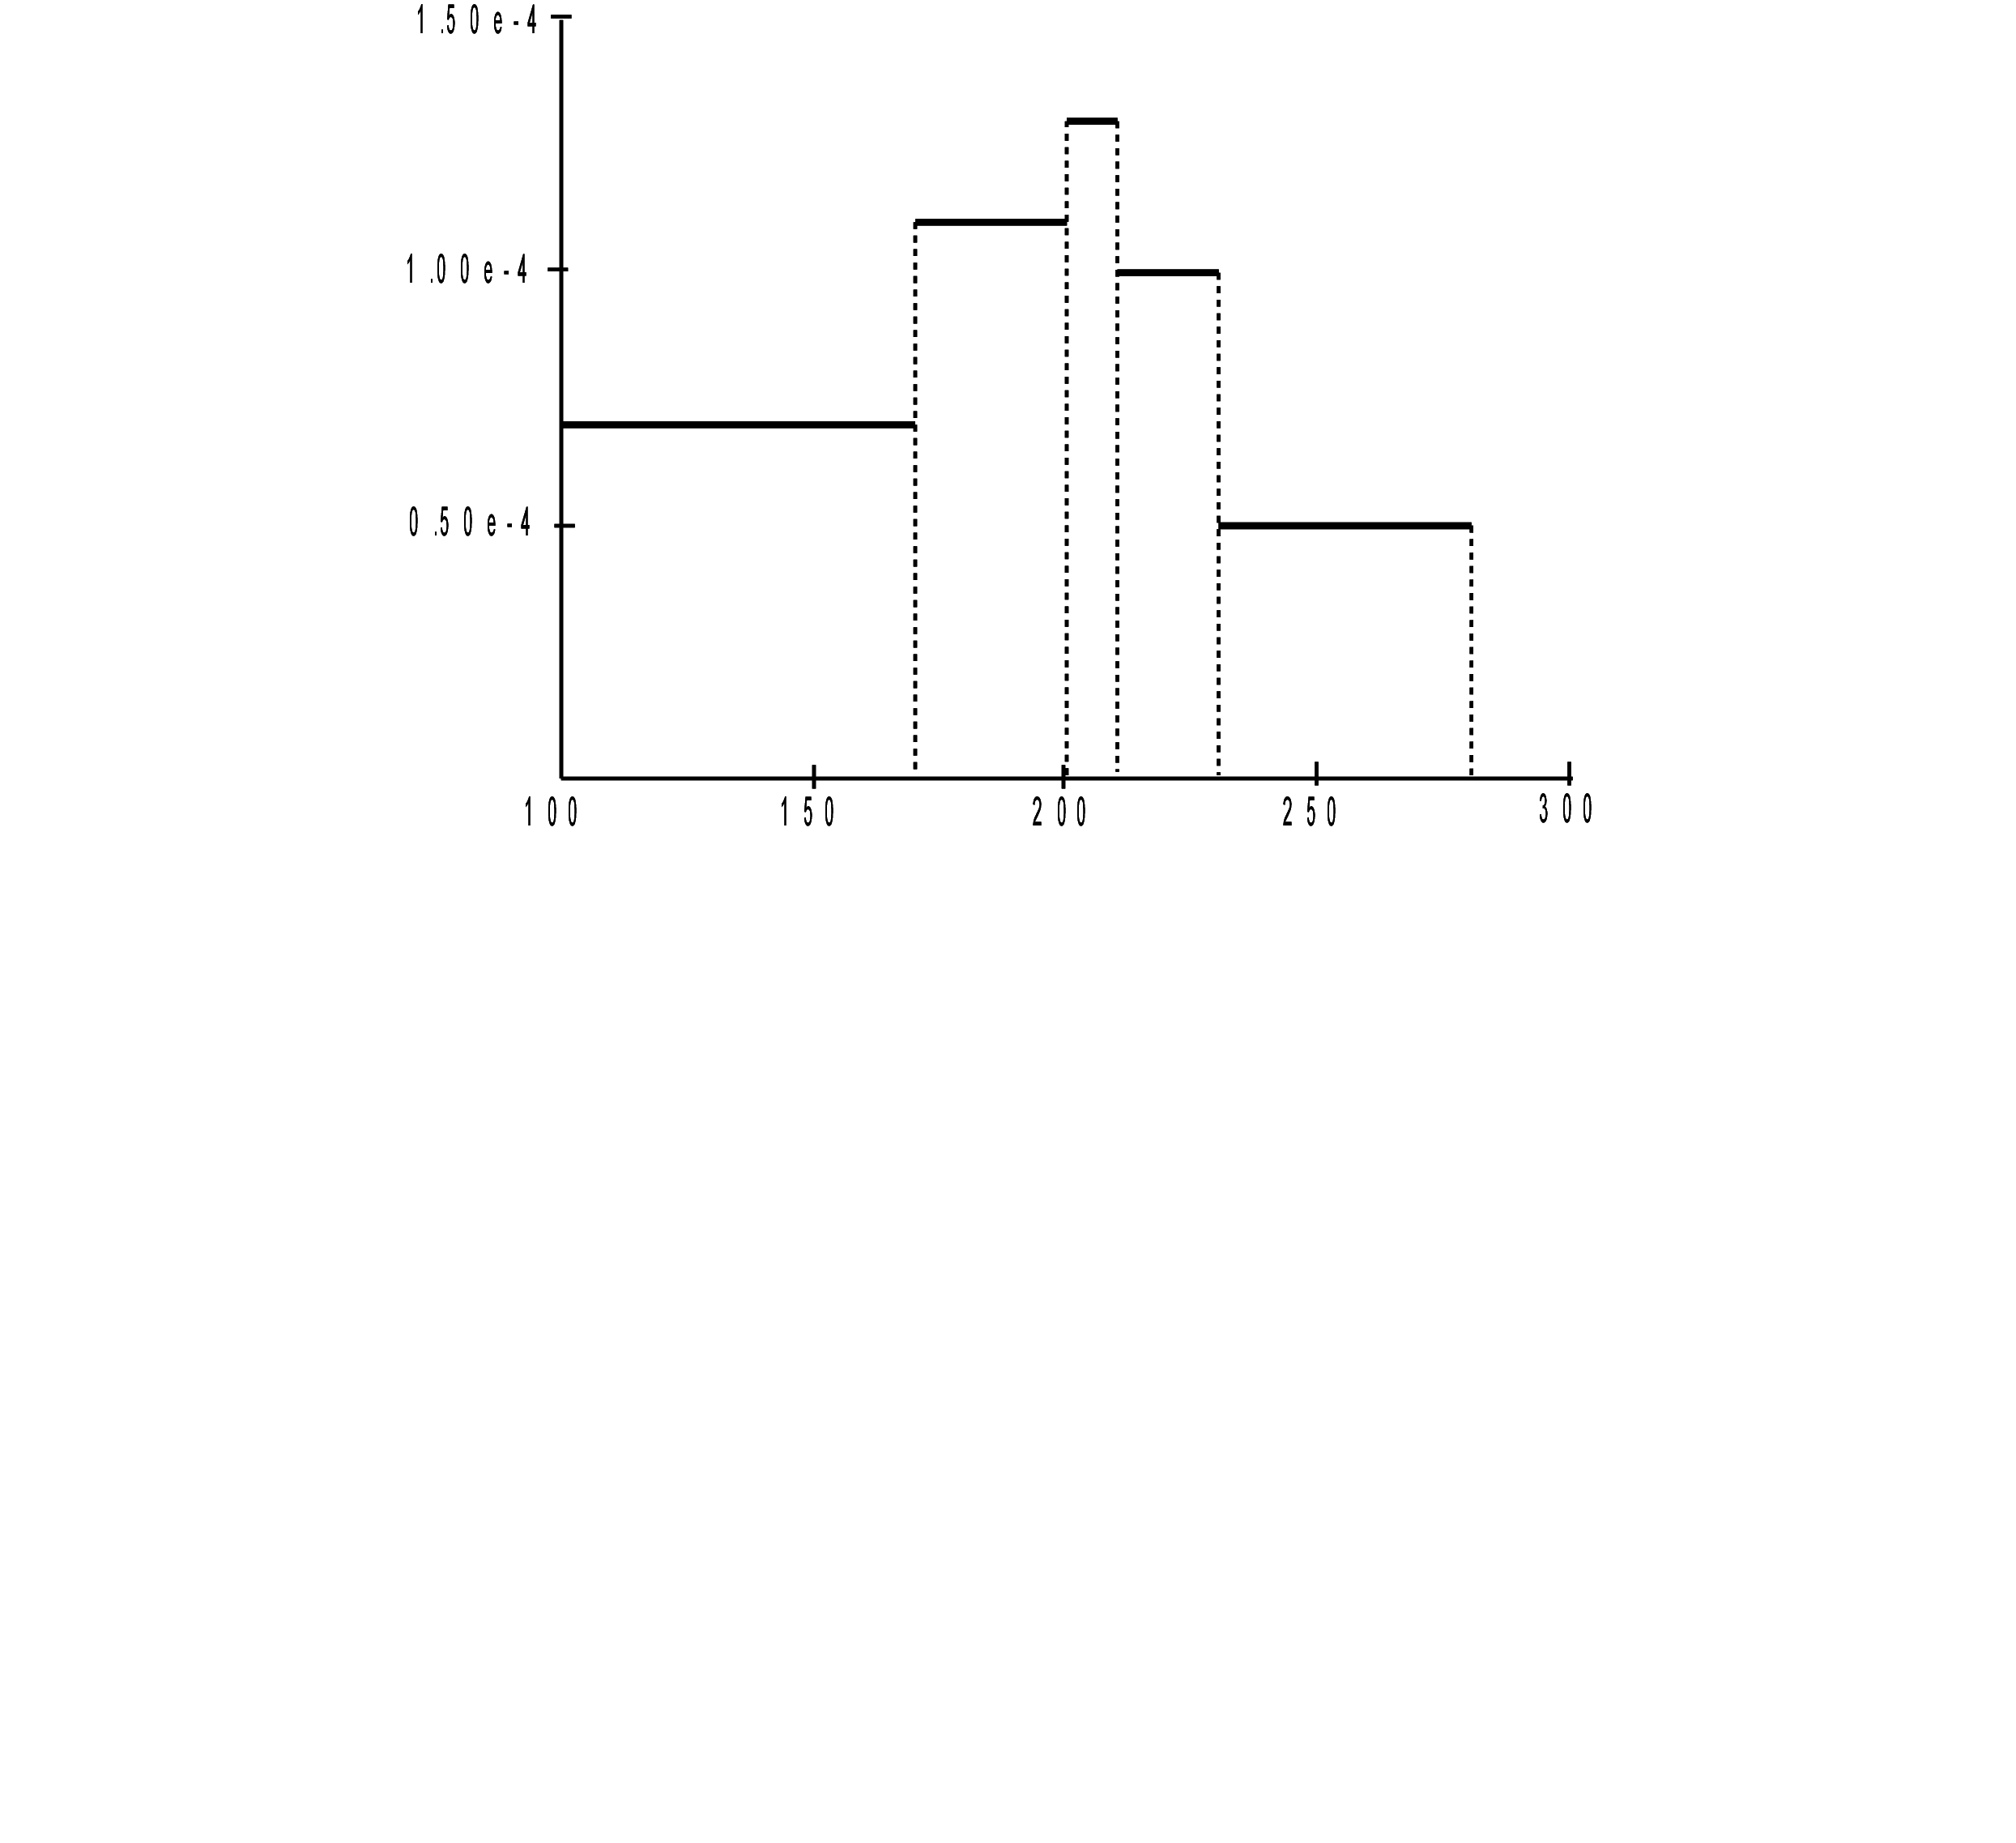
\includegraphics[width=0.9\textwidth]{./word/media/image9.png}
\caption{\label{fig:org9bcb430}
}
\end{figure}

The XML encoding for ``lambda'' is as follows.
\lstset{language=XML,label= ,caption= ,captionpos=b,numbers=none}
\begin{lstlisting}
<define-parameter name="lambda" >
  <histogram>
    <float value"100" />
    <bin> 
      <float value"170" /> 
      <float value="0.70e-4" /> 
    </bin>
    <bin> 
      <float value"200" /> 
      <float value="1.10e-4" /> 
    </bin>
    <bin> 
      <float value"210" /> 
      <float value="1.30e-4" /> 
    </bin>
    <bin> 
      <float value"230" /> 
      <float value="1.00e-4" /> 
    </bin>
    <bin> 
      <float value"280" /> 
      <float value="0.50e-4" /> 
    </bin>
  </histogram>
</define-parameter>
\end{lstlisting}

\subsection{Directives to Test the Status of Initiating and Functional Events}
\label{sec:orgcde4bc8}



\subsubsection{Description}
\label{sec:orgd838606}

The Model Exchange Format provides two special directives to test
whether a given initiating event occurred and whether a given functional
event is in a given state. The meaning of these directives will be
further explained Section VII.3.

Table IV -1 presents these directives and their arguments.



\begin{table}[htbp]
\caption{Directives to test the status of initiating and functional events \label{TableV-6}}
\centering
\begin{tabular}{lrl}
\textbf{Built-in} & \textbf{\#arguments} & \textbf{Semantics}\\
\textbf{test-initiating-event} & 1 & <test-initiating-event name="name" /> returns true if the initiating event of the given name occurred.\\
\textbf{test-functional-event} & 2 & <test-functional-event name="name" state="state" /> returns true if the functional event of the given name is in the given state.\\
\end{tabular}
\end{table}


\subsubsection{XLM Representation}
\label{sec:org14ce188}

The XML representation for directives to test the status of initiating
and functional events is given Figure \ref{FigureV-19}.

\lstset{language=[LaTeX]TeX,label= ,caption={Backus-Naur grammar for XML representation of directives to test the status of initiating and functional events \label{FigureV-19}.},captionpos=b,numbers=none}
\begin{lstlisting}
test-event ::=
  <test-initiating-event name="name" />
  | <test-functional-event name="/name/" state="/identifier/" />
\end{lstlisting}

\section{Meta-Logical Layer}
\label{sec:orgd50e44e}

The meta-logical layer is populated constructs like common cause groups,
delete terms, recovery rules, and exchange events that are used to give
flavors to fault trees. This chapter reviews all of these constructs.

\subsection{Common Cause Groups}
\label{sec:orge955582}


\subsubsection{Description}
\label{sec:org82b346e}

From a theoretical view point, one of the basic assumptions of the fault
tree technique is that occurrences of basic events are independent from
a statistical viewpoint. However, most of the PSA models include, to a
large extent, so-called common cause groups. Common cause groups are
groups of basic events whose failure are not independent from a
statistical view point. They may occur either independently or
dependently due to a common cause failure. So far, existing tools embed
three models for common cause failures (CCF): the beta-factor model, the
multiple Greek letters (MGL) model and the alpha-factor model.
Alpha-factor and MGL models differ only from the way the factors for
each level (2 components fail, 3 components fail\ldots{}) are given. The
Model Exchange Format proposes the three mentioned models plus a fourth
one, so-called phi-factor, which is a more direct way to set factors.

\emph{Beta-factor:} The \(\beta\)-factor model assumes that if a common cause occurs
then all components of the group fail simultaneously. Components can
fail independently. Multiple independent failures are neglected. The
\(\beta\)-factor model assumes moreover that all of the components of the group
have the same probability distribution. It is characterized by this
probability distribution and the conditional probability \(\beta\) that all
components fail, given that one component failed.

Let BE\(_{\text{1}}\), BE\(_{\text{2}}\)\ldots{} BE\(_{\text{n}}\) be the \emph{n} basic events of a common cause
group with a probability distribution Q and a beta-factor \(\beta\). Applying
the beta-factor model on the fault tree consists in following
operations.

\begin{enumerate}
\item Create new basic events BE\(_{\text{CCFi}}\) for each BE\(_{\text{i}}\) to represent the
independent occurrence of BE\(_{\text{i}}\) and BE\(_{\text{CCFi}}\) to represent the
occurrence of all BE\(_{\text{i}}\) together.

\item Substitute a gate ``G\(_{\text{i}}\) = BE\(_{\text{CCFi}}\) or BE\(_{\text{i}}\)'' for each basic event
BE\(_{\text{i}}\).

\item Associate the probability distribution (e.g. \(\beta\)\texttimes{} Q) with the event
BE\(_{\text{CCFi}}\).
\end{enumerate}

\emph{Multiple Greek Letters:} the Multiple Greek Letters (MGL) model
generalizes the beta-factor model. It considers the cases where
sub-groups of 1, 2\ldots{}, n-1 components of the group fail together. This
model is characterized by the probability distribution of failure of the
components, and n-1 factors \(\rho_{\text{2}}\)\ldots{}, \(\rho_{\text{n}}\). \(\rho_{\text{k}}\) denotes the
conditional probability that k components of the group fail given that
k-1 failed.

Let BE\(_{\text{1}}\), BE\(_{\text{2}}\)\ldots{} BE\(_{\text{n}}\) be the \emph{n} basic events of a common cause
group with a probability distribution Q and factors \(\rho_{\text{2}}\)\ldots{}, \(\rho_{\text{n}}\).
Applying the MGL model on the fault tree consists in following
operations.

\begin{enumerate}
\item Create a basic event for each combination of basic events of the
group (there are 2/\(^{\text{n}}\)/-1 such combinations).

\item Transform each basic event BE\(_{\text{i}}\) into a OR-gate G\(_{\text{i}}\) over all newly
created event basic events that represent a group that contains
BE\(_{\text{i}}\).

\item Associate the following probability distribution with each newly
created basic event representing a group of \emph{k} components (with
\(\rho_{\text{n+1}}\)=0).
\end{enumerate}

For instance, for a group of 4 basic events: A, B, C and D, the basic
event A is transformed into a gate G\(_{\text{A}}\) = A or AB or AC or AD or ABC or
ABD or ACD or ABDC and the Q\(_{\text{k}}\)'s are as follows.

Note that if \(\rho_{\text{k}}\)=0 then Q\(_{\text{k}}\), Q\(_{\text{k+1}}\)\ldots{}are null as well. In such a
case it is not necessary to create the groups with k elements or more.

\emph{Alpha-Factor:} the alpha-factor model is the same as the MGL model
except in the way the factors are given. Here \emph{n} factors \(\alpha_{\text{1}}\)\ldots{}\(\alpha_{\text{n}}\)
are given. \(\alpha_{\text{k}}\) represents the fraction of the total failure
probability due to common cause failures that impact exactly \emph{k}
components. The distribution associated with a group of size \emph{k} is as
follows:

\emph{Phi-Factor:} the phi-factor model is the same as MGL and alpha-factor
models except that factors for each level are given directly.

Indeed the sum of the \(\phi_{\text{i}}\)'s should equal 1.

\subsubsection{XML representation}
\label{sec:org5fd2bfc}

The Backus-Naur form for the XML description of Common Cause Failure
Groups is given Figure VI -20. Note that the number of factors depends
on the model. Tools are in charge of checking that there is the good
number of factors. Note also that each created basic event is associated
with a factor that depends on the model and the level of the basic
event. The sum of the factors associated with basic events of a member
of the CCF group should be equal to 1, although this is not strictly
required by the Model Exchange Format.

\lstset{language=[LaTeX]TeX,label= ,caption={Backus-Naur form for the XML representation of CCF-groups \label{FigureVI-20}.},captionpos=b,numbers=none}
\begin{lstlisting}
CCF-group-definition ::=
  <define-CCF-group name="identifier" model="CCF-model" >
  [ label ]
  [ attributes ]
  members
  distribution
  factors
  </define-CCF-group>

members ::=
  <members>
  <basic-event name="identifier" />+
  </members>
  factors ::=
<factors> factor+ </factors>
  | factor
factor ::=
  <factor [ level="integer" ] >
  expression
  </factor>
distribution ::=
  <distribution >
  expression
  </distribution>
CCF-model ::= beta-factor | MGL | alpha-factor | phi-factor
\end{lstlisting}



\emph{Example:} Here follows a declaration of a CCF-group with four elements
under the MGL model.

\lstset{language=XML,label= ,caption= ,captionpos=b,numbers=none}
\begin{lstlisting}
<define-CCF-group name="pumps" model="MGL" >
  <members>
    <basic-event name="pumpA" />
    <basic-event name="pumpB" />
    <basic-event name="pumpC" />
    <basic-event name="pumpD" />
  </members>
  <factors>
    <factor level="2" >
      <float value="0.10" />
    </factor>
    <factor level="3" >
      <float value="0.20" />
    </factor>
    <factor level="4" >
      <float value="0.30" />
    </factor>
  </factors>
  <distribution>
    <exponential>
      <parameter name="lambda" />
      <system-mission-time />
    </exponential>
  </distribution>
</define-CCF-group>
\end{lstlisting}



\subsection{Delete Terms, Recovery Rules and Exchange Events}
\label{sec:org84f9713}

\subsubsection{Description}
\label{sec:org51d0d1a}

\emph{Delete Terms:} Delete Terms are groups of pair wisely exclusive basic
events. They are used to model impossible configurations. A typical
example is the case where:

\begin{itemize}
\item the basic event a can only occur when the equipment A is in
maintenance,

\item the basic event b can only occur when the equipment B is in
maintenance,

\item equipments A and B are redundant and cannot be simultaneously in
maintenance.
\end{itemize}

In most of the tools, delete terms are considered as a post-processing
mechanism: minimal cutsets containing two basic events of a delete terms
are discarded. In order to speed-up calculations, some tools use basic
events to discard minimal cutsets on the fly, during their generation.

Delete Terms can be handled in several ways. Let G = \{e\(_{\text{1}}\), e\(_{\text{2}}\),
e\(_{\text{3}}\)\} be a Delete Term (group).

\begin{itemize}
\item A first way to handle G, is to use it to post-process minimal
cutsets, or to discard them on the fly during their generation. If a
minimal cusets contains at least two of the elements of G, it is
discarded.

\item A global constraint ``C\(_{\text{G}}\) = not 2-out-of-3(e\(_{\text{1}}\), e\(_{\text{2}}\), e\(_{\text{3}}\))'' is
introduced and each top event (or event tree sequences) ``top'' is
rewritten as ``top and C\(_{\text{G}}\)''.

\item As for Common Causes Groups, the e\(_{\text{i}}\)'s are locally rewritten in as
gates:

\begin{itemize}
\item e\(_{\text{1}}\) is rewritten as a gate ge\(_{\text{1}}\) = e\(_{\text{1}}\) and (not e\(_{\text{2}}\)) and
(not e\(_{\text{3}}\))

\item e\(_{\text{2}}\) is rewritten as a gate ge\(_{\text{2}}\) = e\(_{\text{2}}\) and (not e\(_{\text{1}}\)) and
(not e\(_{\text{3}}\))

\item e\(_{\text{3}}\) is rewritten as a gate ge\(_{\text{3}}\) = e\(_{\text{3}}\) and (not e\(_{\text{1}}\)) and
(not e\(_{\text{2}}\))
\end{itemize}
\end{itemize}

\emph{Recovery Rules:} Recovery Rules are an extension of Delete Terms. A
Recovery Rule is a couple (H, e), where H is a set of basic events and e
is a (fake) basic event. It is used to post-process minimal cutsets: if
a minimal cutset C contains H, the e is added to C. Recovery Rules are
used to model actions taken in some specific configurations to mitigate
the risk (hence their name).

Here several remarks can be made.

\begin{itemize}
\item It is possible to mimics Delete Terms by means of recovery rules. To
do so, it suffices to assign the basic event e to the value ``false''
or the probability 0.0.

\item As for Delete Terms, it is possible to give purely logical
interpretation to Recovery Rules. The idea is to add a global
constraint ``H \(\rightarrow\) e'', i.e. ``not H or e'', for each Recovery Rule (H, e).

\item Another definition of Recovery Rules as a post-processing is that the
event e is substituted for subset H in the minimal cutset. This
definition has however the major drawback to be impossible to
interpret in a logical way. No Boolean formula can withdraw events
from a configuration.
\end{itemize}

\emph{Exchange Events:} Exchange Events are very similar to Recovery Rules.
An Exchange Event (Rule) is a triple (H, e, e'), where H is a set of
basic events and e and e' are two basic events. Considered as a
post-processing of minimal cutsets, such a rule is interpreted as
follows. If the minimal cutset contains both the set H and the basic
event e, then the basic event e' is substituted for e in the cutset. For
the same reason as above, Exchange Events cannot be interpreted in a
logical way.

\subsection{All Extra-Logical Constructs in One: the Notion of Substitution}
\label{sec:org4409979}

Constructs that cannot be interpreted in a logical way should be avoided
for at least two reasons. First, models containing such constructs are
not declarative. Second and more importantly, they tighten assessment
tools to one specific type of algorithms. The second interpretation of
Recovery Rules and Exchange Events tighten the models to be assessed by
means of the minimal cutsets approach.

Nevertheless, Recovery Rules and Exchange Events are useful and broadly
used in practice. Fortunately, Exchange Events (considered as a post
processing mechanism) can be avoided in many cases by using the
instructions that give flavors to fault trees while walking along event
tree sequences: in a given sequence, one may decide to substitute the
event e' for the event e (or the parameter p' for the parameter p) in
the Fault Trees collected so far. This mechanism is perfectly acceptable
because it applies while creating the Boolean formula to be assessed.

It is not yet possible to decide whether Recovery Rules (under the
second interpretation) and Exchange Events can be replaced by purely
declarative constructs or by instructions of event trees. This has to be
checked on real-life models. To represent Delete Term, Recovery Rules
and Exchange Events, the Model Exchange Format introduces a unique
construct: the notion of substitution.

A substitution is a triple (H, S, t) where:

\begin{itemize}
\item H, the hypothesis, is a (simple) Boolean formula built over basic
events,

\item S, the source, is also a possibly empty set of basic events, and
finally

\item t, the target, is either a basic event or a constant.
\end{itemize}

Let C be a minimal cutset, i.e. a set of basic events. The substitution
(H, S, t) is applicable on C if C satisfies H (i.e. if H is true when C
is realized) . The application of (H, S, t) on C consists in removing
from C all the basic events of S and in adding to C the target t.

Note that if t is the constant ``true'', adding t to C is equivalent to
add nothing. If t is the constant ``false'' adding t to C is equivalent to
discard C.

This notion of substitution generalizes the notions of Delete Terms,
Recovery Rules and Exchange Events:

\begin{itemize}
\item Let D = \{e\(_{\text{1}}\), e\(_{\text{2}}\)\ldots{}, e\(_{\text{n}}\)\} be a group of pair wisely exclusive
events (a Delete Term). Then D is represented as the substitution
(2-out-of-n(e\(_{\text{1}}\), e\(_{\text{2}}\)\ldots{}, e\(_{\text{n}}\)), \(\emptyset\), false).

\item Let (H, e) a Recovery Rule, under the first interpretation, where H =
\{e\(_{\text{1}}\), e\(_{\text{2}}\)\ldots{}, e\(_{\text{n}}\)\}. Then, (H, e) is represented by the
substitution (e\(_{\text{1}}\) and e\(_{\text{2}}\) and\ldots{}and e\(_{\text{n}}\), \(\emptyset\), e).

\item Let (H, e) a Recovery Rule, under the second interpretation, where H
= \{e\(_{\text{1}}\), e\(_{\text{2}}\)\ldots{}, e\(_{\text{n}}\)\}. Then (H, e) is represented by the
substitution (e\(_{\text{1}}\) and e\(_{\text{2}}\) and\ldots{}and e\(_{\text{n}}\), H, e).

\item Finally, let (H, e, e') be an Exchange Event Rule, where H = \{e\(_{\text{1}}\),
e\(_{\text{2}}\)\ldots{}, e\(_{\text{n}}\)\}. Then (H, e, e') is represented by the substitution
(e\(_{\text{1}}\) and e\(_{\text{2}}\) and\ldots{}and e\(_{\text{n}}\) and e, \{e\}, e').
\end{itemize}

Note that a substitution (H, \(\emptyset\), t) can always be interpreted as the
global constraint ``H \(\rightarrow\) t''.

\subsubsection{XML Representation}
\label{sec:org21881f9}

The Backus-Naur form for the XML description of substitutions is given
Figure VI -21. The optional attribute ``type'' is used to help tools that
implement ``traditional'' substitutions.

\lstset{language=[LaTeX]TeX,label= ,caption={Backus-Naur form for the XML representation of exclusive-groups \label{FigureVI-21}.},captionpos=b,numbers=none}
\begin{lstlisting}
substitution-definition ::=
  <define-substitution [ name="identifier" ] [ type="identifier" ] >
    [ label ] [ attributes ]
    <hypothesis> Boolean-formula <hypothesis>
    [ <source> basic-event+ <source> ]
    <target> basic-event+ | Boolean-constant <target>
  <define-substitution >
\end{lstlisting}



\emph{Example:} Assume that Basic Events ``failure-pump-A'', ``failure-pump-B''
and ````failure-pump-C'' are pair wisely exclusive (they form a delete
term) because they can only occur when respectively equipment A, B and C
are under maintenance and only one equipment can be in maintenance at
once. The representation of such a delete term is as follows.


\lstset{language=XML,label= ,caption= ,captionpos=b,numbers=none}
\begin{lstlisting}
<define-substitution name="pumps" type="delete-terms" >
  <hypothesis>
    <atleast min="2">
      <basic-event name="failure-pump-A" />
      <basic-event name="failure-pump-B" />
      <basic-event name="failure-pump-C" />
    </atleast>
  </hypothesis>
  <target>
    <constant value="false" />
    <target>
    </define-substitution >
\end{lstlisting}

\emph{Example:} Assume that if the valve V is broken and an overpressure is
detected in pipe P, then a mitigating action A is performed. This is a
typical Recovery Rule (under the first interpretation), where the
hypothesis is the conjunction of Basic Events ``valve-V-broken'' and
``overpressure-pipe-P'' and the added Basic Event is ``failure-action-A''.
It is encoded as follows.


\lstset{language=XML,label= ,caption= ,captionpos=b,numbers=none}
\begin{lstlisting}
<define-substitution name="mitigation" type="recovery-rule" >
  <hypothesis>
    <and>
      <basic-event name="valve-V-broken" />
      <basic-event name="overpressure-pipe-P" />
    </and>
  </hypothesis>
  <target>
    <basic-event name="failure-action-A" />
    <target>
    </define-substitution >
\end{lstlisting}

\emph{Example:} Assume that if magnitude of the earthquake is 5, 6 or 7, the
size of a leak of a given pipe P get large, while it was small for
magnitudes below 5. We can use an exchange event rule to model this
situation.

\lstset{language=XML,label= ,caption= ,captionpos=b,numbers=none}
\begin{lstlisting}
<define-substitution name="magnitude-impact" type="exchange-event" >
  <hypothesis>
    <or>
      <basic-event name="magnitude-5" />
      <basic-event name="magnitude-6" />
      <basic-event name="magnitude-7" />
    </or>
  </hypothesis>
  <source>
    <basic-event name="small-leak-pipe-P" />
    <source>
      <target>
	<basic-event name="large-leak-pipe-P" />
	<target>
	</define-substitution >
\end{lstlisting}

\section{Event Tree Layer}
\label{sec:orgb8a1051}


\subsection{Preliminary Discussion}
\label{sec:org0e50411}

The first three layers are rather straightforward to describe since
there is a general agreement on how to interpret fault trees and
probability distributions. The Event Tree layer is much more delicate to
handle. The reason stands in the dynamic nature of event trees and the
lack of common interpretation for this formalism. To illustrate this
point, we shall consider the toy example pictured Figure \ref{im-small-et}.


\begin{figure}[htbp]

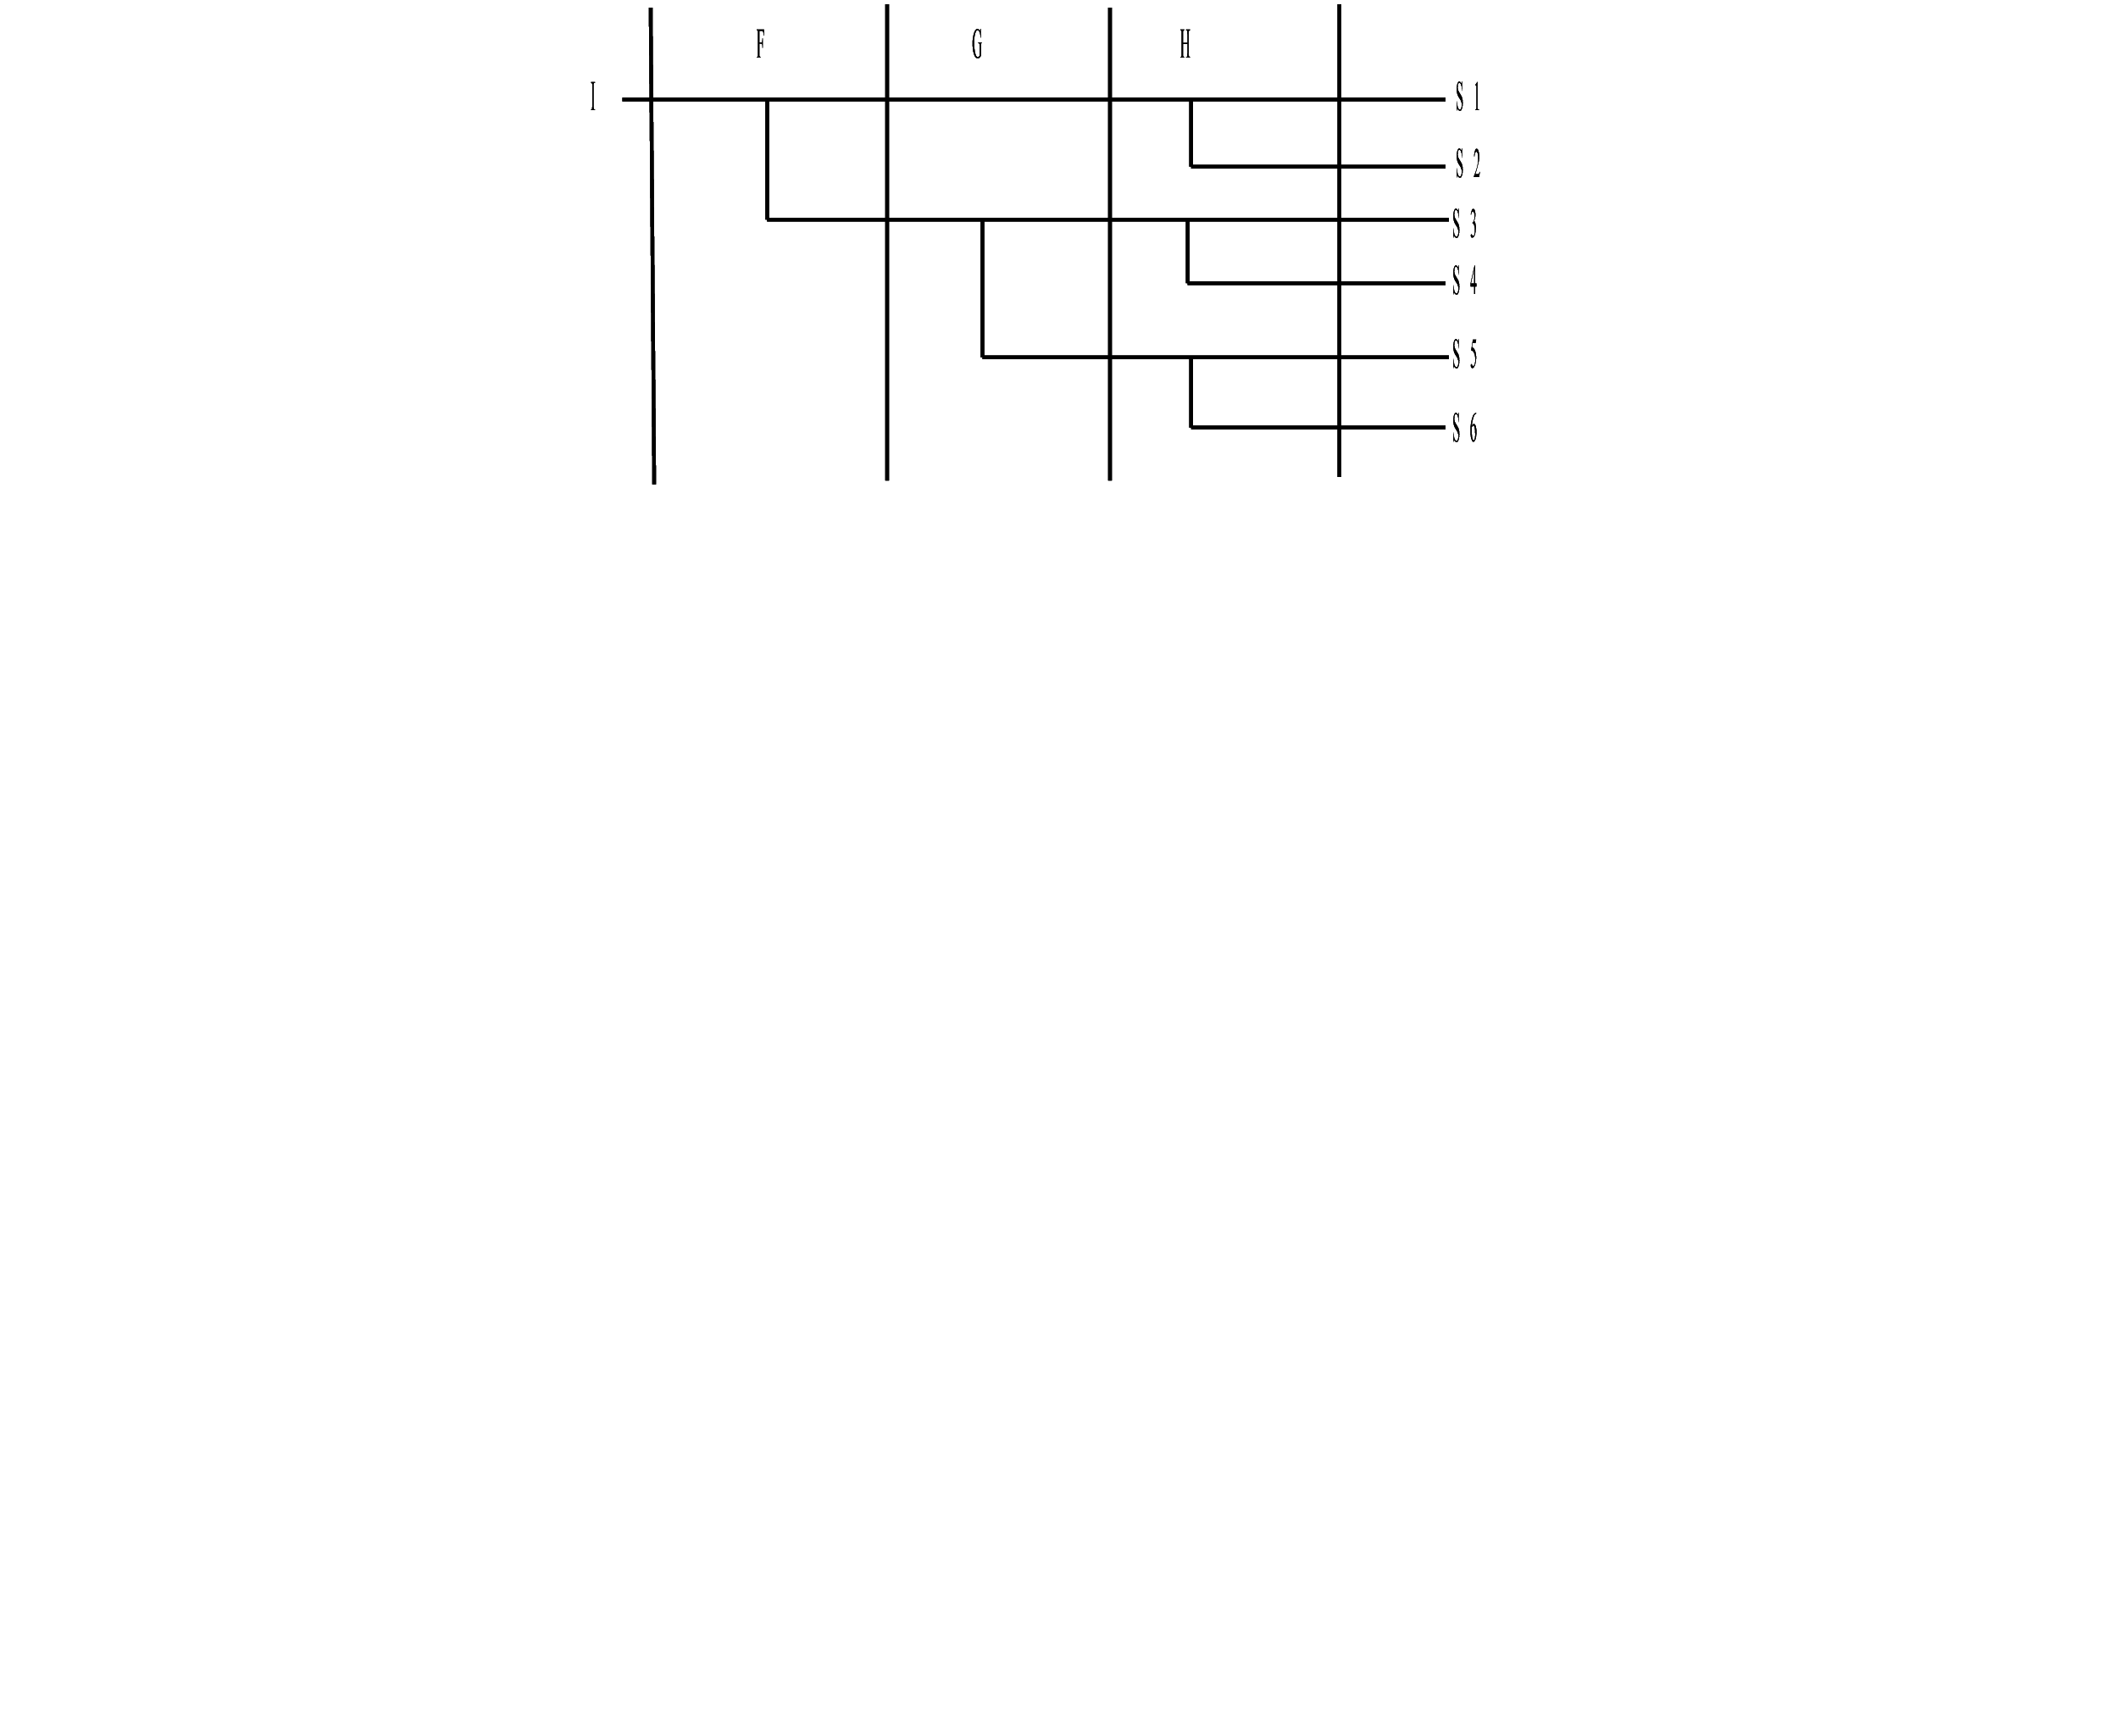
\includegraphics[width=0.9\textwidth]{./word/media/image10.png}
\caption{\label{fig:org33bca25}
A Small Event Tree}
\end{figure}

This event tree is made of the following elements.

\begin{itemize}
\item An initiating event I.

\item Three functional events F, G and H.

\item Six sequences ending in six (a priori) different states S1 to S6.
\end{itemize}

The numbered black dots should be ignored for now. We added them only
for the convenience of the forthcoming discussion.

The expected interpreted interpretation of this event tree is as
follows. A fault tree is associated with each functional event. This
fault tree describes how the functional event may occur. For the sake of
the simplicity, we may assume that its top-event has the same name as
the functional event itself. Upper branches represent a success of the
corresponding safety mission while lower branches represent its failure.
Applying the so-called fault tree linking approach, we obtain the
following interpretation for the sequences.

S1 = I and not F and not H S4 = I and F and not G and H

S2 = I and not F and H S5 = I and F and G and not F

S3 = I and F and not G and not H S6 = I and F and G and H

In practice, things are less simple:

\begin{itemize}
\item There may be more that one initiating event, because the same event
tree can be used with different flavors.

\item Values of house events may be changed at some points along the
branches to give flavors to fault trees. The value of a house event
may be changed either locally to a fault tree, or for all the fault
trees encountered after the setting point.

\item The flavoring mechanism may be even more complex: some gates or basic
events may be negated; some parameters of probability distributions
may be impacted.

\item The flavor given to a fault tree may depend on what has happened so
far in the sequence: initiating event, value of house events\ldots{}

\item Some success branches may not be interpreted as the negation of the
associated fault tree but rather as a bypass. This interpretation of
success branches is typically tool-dependent: some tools (have
options to) ignore success branches; therefore modelers use this
``possibility'' to ``factorize'' models.

\item Branching may have more than two alternatives, or represent
multi-states, not just success and failure, each alternative being
labeled with a different fault tree.

\item In the event tree linking approach, branching may involve no fault
tree at all, but rather a multiplication by some factor of the
current probability of the sequence.

\item It is sometimes convenient to replace a sub-tree by a reference to a
previously define sub-tree. For instance, if we identify end-states
S1 and S3 one the one hand, S2 and S4 on the other hand, we can merge
the two corresponding sub-trees rooted. It saves space (both in
computer memory and onto the display device) to replace the latter by
a reference to the former.
\end{itemize}

In a word, event trees cannot be seen as a static description formalism
like fault trees. Rather, they should be seen as a kind of graphical
programming language. This language is used to collect and modify data
when walking along the sequences, and even to decide when to stop to
walk a sequence (in the event tree linking approach). The Model Exchange
Format should thus reflect this programming nature of event trees.

\subsection{Structure of Event Trees}
\label{sec:orga71c6b1}



\subsubsection{Description}
\label{sec:org7bc2b38}

The Model Exchange Format distinguishes the structure of the event
trees, i.e. the set of sequences they encode, from what is collected
along the sequences and how it is collected. Let us consider for now
only the structural view point. With that respect, an event tree is made
of the following components.

\begin{itemize}
\item One or more initiating events;

\item An ordered set of functional events (the columns);

\item A set of end-states (so called sequences); and finally

\item A set of branches to describe sequences.
\end{itemize}

Branches end up either with a sequence name, or with a reference to
another branch (such references are sometimes called transfers). They
contain forks. Each fork is associated with a functional event. The
initiating event could also be seen as a special fork (between the
occurrence of this event and the occurrence of \ldots{} no event). In the
Model Exchange Format, alternatives of the fork are called paths. Paths
are labeled by state of the functional event that labels the fork.

Let us consider again the event tree pictured Figure \ref{im-small-et}. Assume
that end states S1 and S3 on the one hand, S2 and S4 and the other hand
are identical and that we merge the corresponding sub-trees. Assume
moreover that the lowest success branch of the functional event H is
actually a bypass. Then, the structure of the tree is pictured Figure \ref{im-str-et}
VII -23. On this figure, nodes of the tree are numbered from 1 to 8. The
initiating event is represented as a fork. Finally, the branch (the
sub-tree) rooted by the node 2 is named B1.


\begin{figure}[htbp]

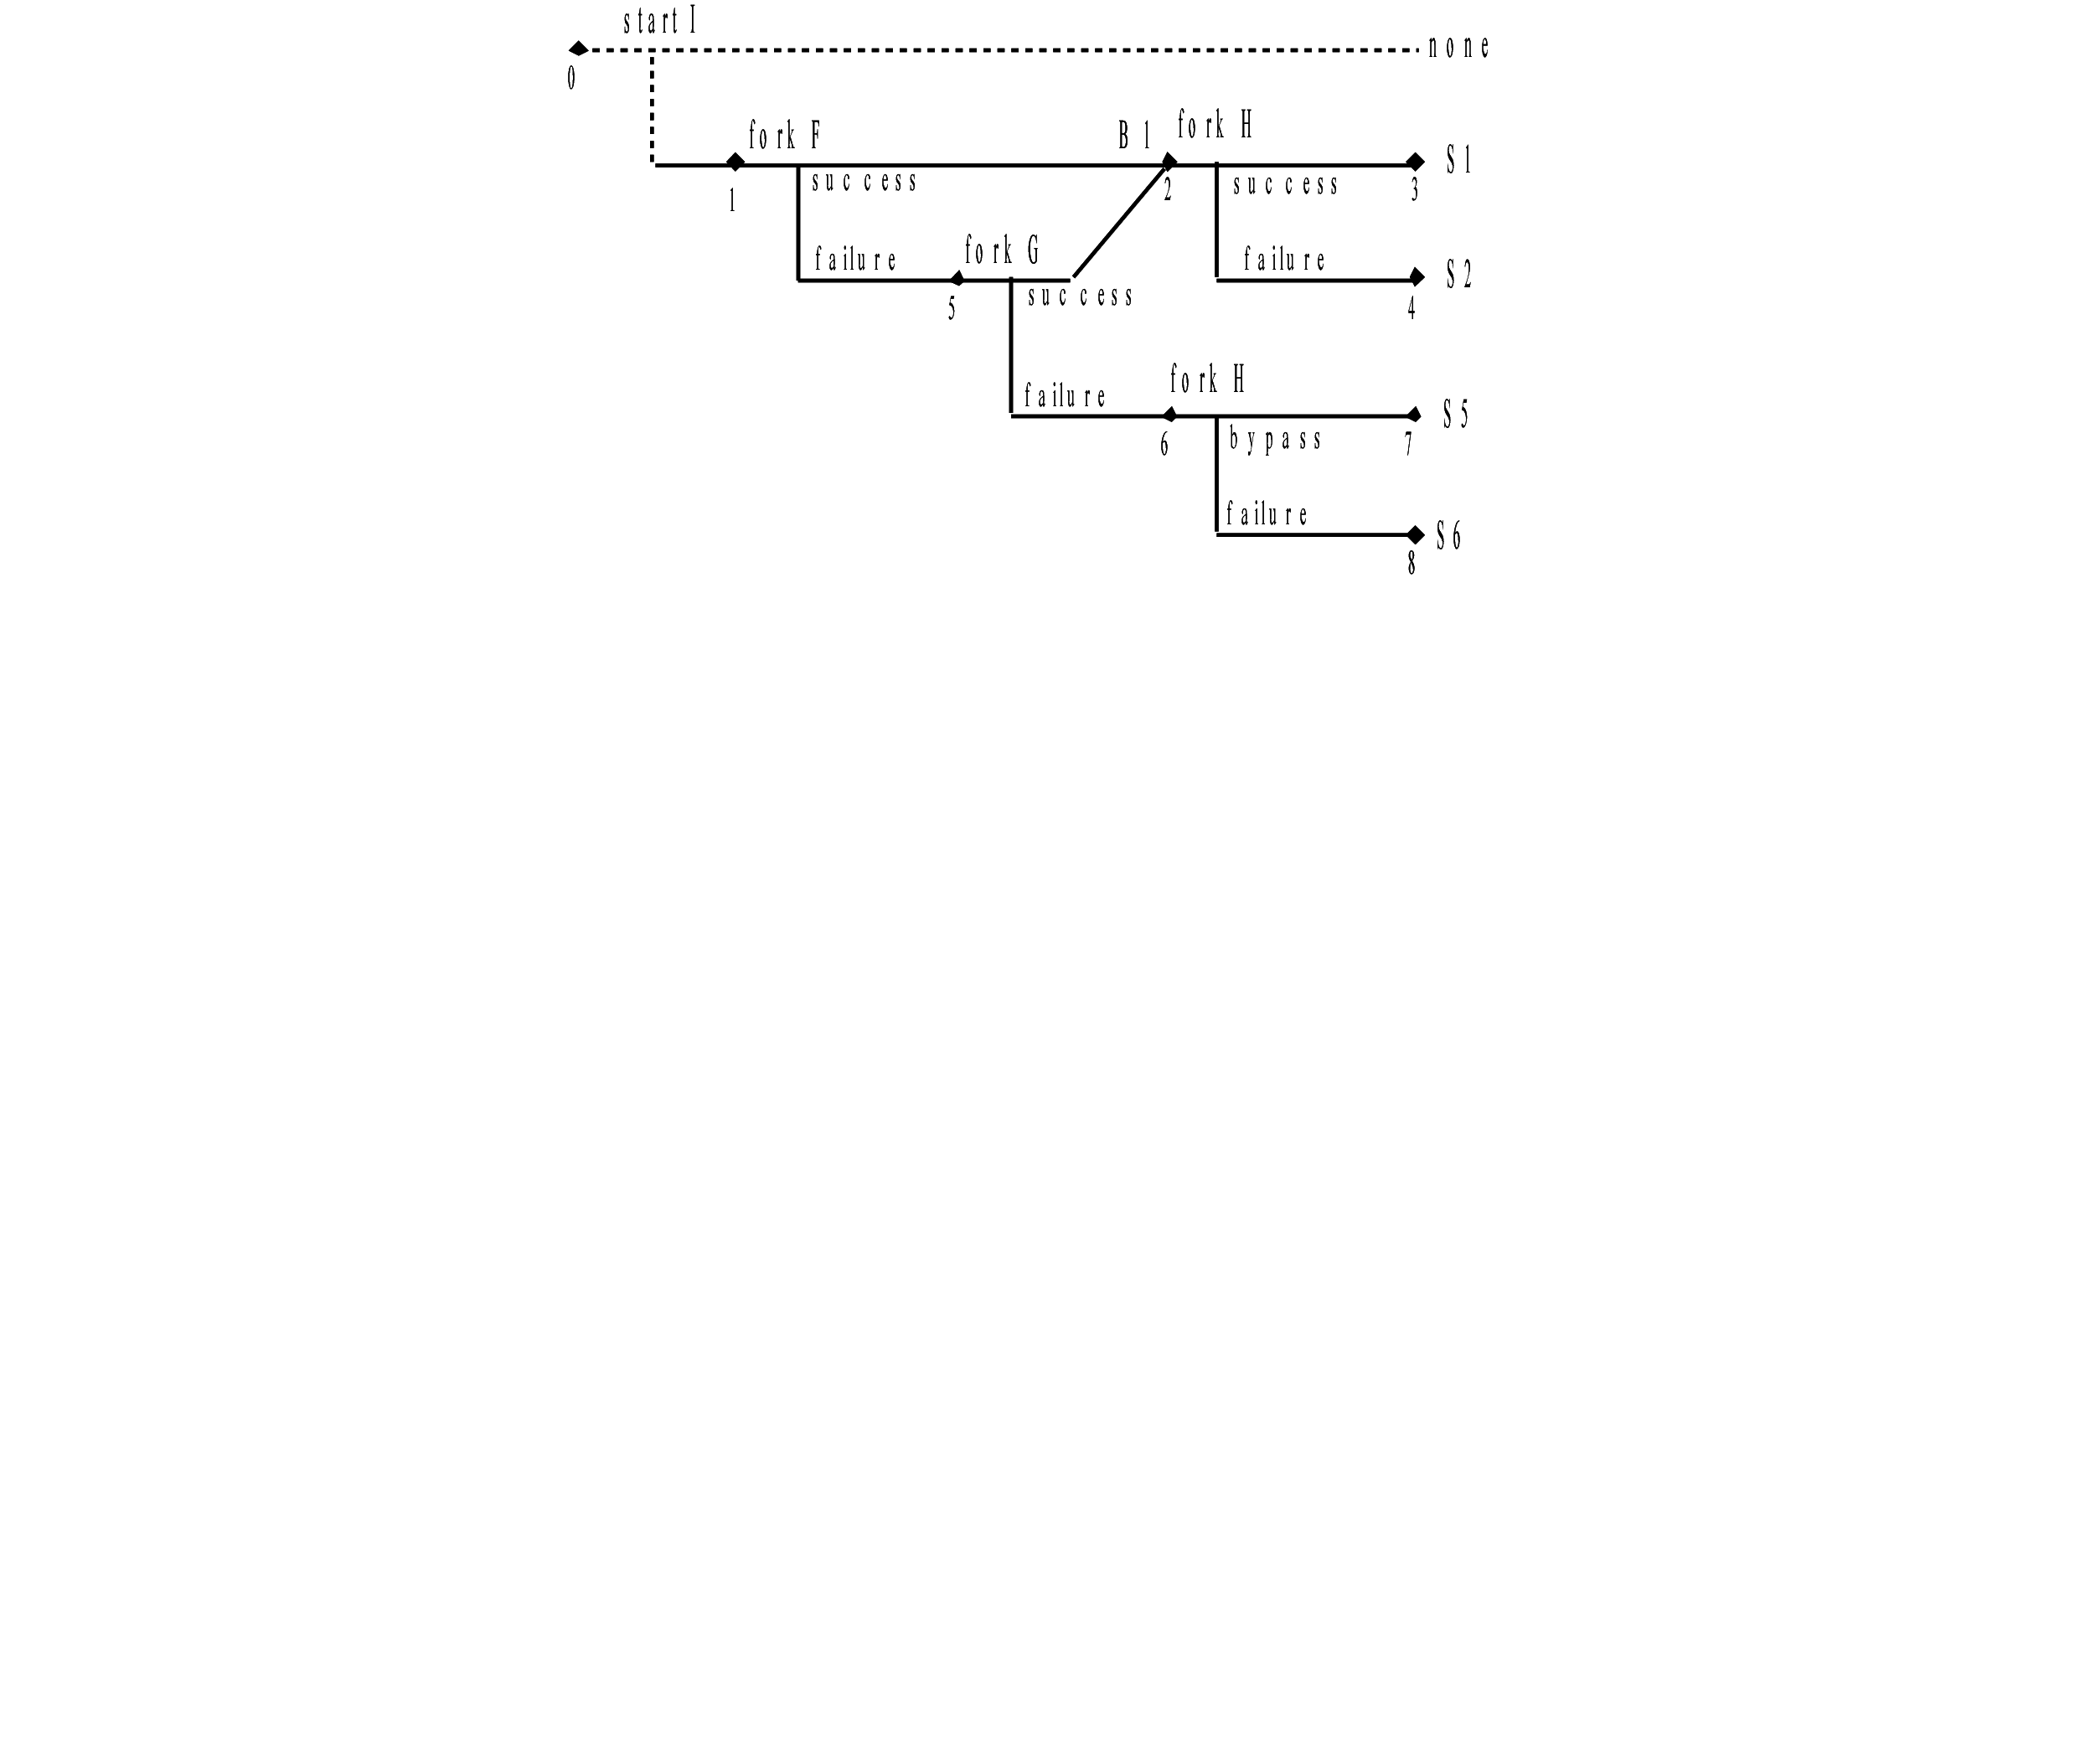
\includegraphics[width=0.9\textwidth]{./word/media/image11.png}
\caption{\label{fig:org606a140}
Structure of an Event Tree}
\end{figure}

Components of the event tree pictured Figure \ref{im-str-et} are the following.

\begin{itemize}
\item The initiating event I.

\item The three functional events F, G and H.

\item The end states S1, S2, S5 and S6.

\item The branch B1.

\item The tree rooted by the initial node (here the node 1).
\end{itemize}

Forks decompose the current branch according to the state of a
functional event. Usually, this state is either ``success'' or ``failure''.
It may be ``bypass'' as well (as in our example for the path from node 6
to node 7). In the case of multiple branches, the name of state is
defined by the user.

Instructions to collect and to modify fault trees and probability
distributions are applied at the different nodes. Instructions to be
applied may depend on the initiating event and the states of functional
events.

The states of functional events at a node depend on the path that has
been followed from the root node to this node. By default, functional
events are in an unspecified state, i.e. that the predicate
``test-functional-event'' (see section V.5) returns false in any case.
Table \ref{TableVII-7} gives the states of functional events for all of the
possible paths starting from the root node of the event tree pictured
Figure \ref{FigureVII-23}. Empty cells correspond to unspecified states.



\begin{table}[htbp]
\caption{States of Functional Events for the different paths of the Event Tree of Figure VII -23 \label{TableVI-I7}.}
\centering
\begin{tabular}{rlll}
\textbf{path} & \textbf{F} & \textbf{G} & \textbf{H}\\
1 &  &  & \\
1-2 & success &  & \\
1-2-3 & success &  & success\\
1-2-4 & success &  & failure\\
1-5 & failure &  & \\
1-5-2 & failure & success & \\
1-5-2-3 & failure & success & success\\
1-5-2-4 & failure & success & failure\\
1-5-6 & failure & failure & \\
1-5-6-7 & failure & failure & bypass\\
1-5-6-8 & failure & failure & failure\\
\end{tabular}
\end{table}



As mentioned above, an event tree may be parametric: the same tree can
be used for several initiating events. To implement this idea, the Model
Exchange Format provides the analyst with the notion of group of
initiating events. Such a group has a name and may contain sub-groups.
Groups of initiating events may be freely defined inside or outside
event trees. There is one condition however: an initiating event can be
used in only one tree.

\subsubsection{XML Representation}
\label{sec:org241e535}

We are now ready to explicitly define the XML grammar of the structure
of event trees. Its Backus-Naur form is given Figure VII -24 and Figure
VII -25. In these figures, we leave instructions unspecified, for they
don't concern the structure of the tree and are the subject of the next
section. Note that branches and functional events cannot be declared
(nor referred to) outside event trees, for there would be no meaning in
doing so.

\lstset{language=[LaTeX]TeX,label= ,caption={Backus-Naur form of the XML representation of initiating events \label{FigureVII-24}.},captionpos=b,numbers=none}
\begin{lstlisting}
initiating-event-definition ::=
  <define-initiating-event name="identifier" [ event-tree="identifier"] >
  [ label ] [ attributes ]
  instruction*
  <define-initiating-event>

initiating-event-group-definition::=
  <define-initiating-event-group name="identifier"
  [event-tree="identifier"] >
  [ label ] [ attributes ]
  initiating-event+
  <define-initiating-event-group>

initiating-event ::=
<initiating-event name="identifier" >
  | <initiating-event-group name="identifier" >
\end{lstlisting}



\lstset{language=[LaTeX]TeX,label= ,caption={Backus-Naur form of the XML representation of event trees and sequences \label{FigureVII-25}.},captionpos=b,numbers=none}
\begin{lstlisting}
event-tree-definition ::=
  <define-event-tree name="identifier" >
  [ label ]
  [ attributes ]
  functional-event-definition*
  sequence-definition*
  branch-definition*
  initial-state
  <define-event-tree>


functional-event-definition ::=
  <define-functional-event name="identifier" >
  [ label ]
  [ attributes ]
  <define-functional-event>

sequence-definition ::=
  <define-sequence name="identifier" >
  [ label ]
  [ attributes ]
  instruction+
  <define-sequence>

branch-definition ::=
  <define-branch name="identifier" >
  [ label ]
  [ attributes ]
  branch
  <define-branch>

initial-state ::=
  <initial-state>
  branch
  <initial-state>

branch ::= instruction* (fork | end-state)
fork ::= <fork functional-event="identifier"> path+ <fork>
path ::= <path state="identifier" > branch <path>
end-state ::=
  <sequence name="identifier" >
  | <branch name="identifier" >
\end{lstlisting}


\emph{Example:} Consider again the event tree pictured Figure \ref{FigureVII-23}. The
XML description for this example is given Figure \ref{FigureVII-26}.


\lstset{language=XML,label= ,caption={XML representation for the structure of the Event Tree pictured Figure \ref{FigureVII-23}  \label{FigureVII-26}.},captionpos=b,numbers=none}
\begin{lstlisting}
<define-event-tree name="my-first-event-tree" >
  <define-functional-event name="F" />
  <define-functional-event name="G" />
  <define-functional-event name="H" />
  <define-sequence name="S1" />
  <define-sequence name="S2" />
  <define-sequence name="S5" />
  <define-sequence name="S6" />
  <define-branch name="sub-tree7" >
    <fork functional-event="H" >
      <path state="success" >
	<sequence name="S1" />
      </path>
      <path state="failure" >
	<sequence name="S2" />
      </path>
    </fork>
    <define-branch>
      <initial-state>
	<fork functional-event="F" >
	  <path state="success" >
	    <branch name="sub-tree7" />
	  </path>
	  <path state="failure">
	    <fork functional-event="G" >
	      <path state="success" >
		<branch name="sub-tree7" />
	      </path>
	      <path state="failure">
		<fork functional-event="H">
		  <path state="success" >
		    <sequence name="S5" />
		  </path>
		  <path state="failure" >
		    <sequence name="S6" />
		  </path>
		</fork>
	      </path>
	    </fork>
	  </path>
	</fork>
      </initial-state>
    </define-event-tree>
\end{lstlisting}


\subsection{Instructions}
\label{sec:org6dbfd75}

\subsubsection{Description}
\label{sec:org3205955}

Figure VII -26 gives the XML representation for the structure of an
event tree. This structure makes it possible to walk along the
sequences, but not to construct the Boolean formulae associated with
each sequences. To do so, we need to fill the structure with
instructions. Instructions are actually used for two main purposes:

\begin{itemize}
\item To collect formulae or stochastic expressions and

\item To define flavors of fault trees and probability distributions, i.e.
to set values of house events and flag parameters.
\end{itemize}

The collection of a top event consists in and-ing the formula associated
with the sequence with a copy of the fault tree rooted with the top
event. In the Model Exchange Format, the operation is performed by means
of the instruction ``collect-formula''. The collection of an expression
multiplies the current probability of the sequence by the value of this
expression. In the Model Exchange Format, the operation is performed by
means of the instruction ``collect-expression''.

To give flavors to fault trees, i.e. to change the values of gates,
house events, basic events and parameters, the Model Exchange Format
introduces the four corresponding instruction: ``set-gate'',
``set-house-event'', ``set-basic-event'' and ``set-parameter''.

Sequences are walked from left to right. Therefore, when a value of an
element is changed, this change applies on the current environment and
propagates to the right. This default behavior can be changed by using
the flag ``direction'', which can take either the value ``forward'' (the
default), ``backward'' or ``both''. This feature should be handled with much
care.

The flavor given to fault trees, as well as what is collected, may
depend on the initial event and the current state of functional events.
To do so, the Model Exchange Format provides an if-then-else instruction
(the ``else'' part is optional) and the two expressions
``test-initial-event'' and ``test-functional-event''. These two instructions
have been introduced Section V.3. Since the then- and else-branches of
the ``if-then-else'' may contain several instructions, the Model Exchange
Format introduces the notion of block of instructions.

Finally, some models require to link event trees. A special instruction
``event-tree'' is introduced for this purpose. It should be used only in
sequence definitions, i.e. in end-state.

It is sometimes the case that the same values of house events and
parameter flags are used at several places. Such a configuration is
called a split-fraction in the event tree linking approach. The Model
Exchange Format refers it as a rule for it is a sequence of
instructions.

\subsection{XML Representation}
\label{sec:org9b245aa}

The Backus-Naur form for the XML representation of instructions is given in Figure \ref{FigureVII-27}.

\lstset{language=[LaTeX]TeX,label= ,caption= ,captionpos=b,numbers=none}
\begin{lstlisting}
instruction ::= set | collect | if-then-else | block | rule |link
set ::= set-gate | set-house-event | set-basic-event | set-parameter
set-gate ::=
  <set-gate name="identifier" [ direction="direction" ] >
  formula
  <set-gate>

set-house-event ::=
  <set-house-event name="identifier" [ direction="direction" ] >
  Boolean-constant
  <set-house-event>
set-basic-event ::=
  <set-basic-event name="identifier" [ direction="direction" ] >
  expression
  <set-basic-event>
set-parameter ::=
  <set-parameter name="identifier" [ direction="direction" ] >
  expression
  <set-parameter>

direction ::= forward | backward | both
if-then-else ::=
  <if> expression instruction [ instruction ] <if>
  collect ::= collect-formula | collect-expression
  collect-formula ::= <collect-formula> formula <collect-formula>
  collect-expression ::= <collect-expression> expression
  <collect-expression>

block ::= <block> instruction* <block>
rule ::= <rule name="identifier" >
link ::= <event-tree name="name" >
rule-definition ::=
  <define-rule name="identifier" >
  [ label ] [ attributes ]
  instruction+
  <define-rule>
\end{lstlisting}

\emph{Example:} Consider again the event tree pictured Figure \ref{FigureVII-23}. The
XML representation for the structure of this tree has been given Figure
\ref{FigureVII-26}. Assume that the success branch of the lower fork on system H is
a bypass. The XML description for the branches of this example is given
Figure \ref{FigureVII-28}. It is easy to verify by traversing this tree by hand so
that it produces the expected semantics.



\lstset{language=XML,label= ,caption={XML representation of the branches of the event tree pictured Figure \ref{FigureVII-23} \label{FigureVII-28}.},captionpos=b,numbers=none}
\begin{lstlisting}
<define-event-tree name="my-first-event-tree" >
  ...
  <initial-state>
    <fork functional-event="F" >
      <path state="success" >
	<collect-formula> 
	  <not> 
	    <gate name="F" > 
	    </not> 
	  </collect-formula>
	  <branch name="sub-tree7" />
	</path>
	<path state="failure" >
	  <collect-formula> 
	    <gate name="F" > 
	    </collect-formula>
	    <fork functional-event="G" >
	      <path state="success" >
		<collect-formula> 
		  <not> 
		    <gate name="G" > 
		    </not> 
		  </collect-formula>
		  <branch name="sub-tree7" />
		</path>
		<path state="failure" >
		  <collect-formula> 
		    <gate name="G" > 
		    </collect-formula>
		    <fork functional-event="H">
		      <path state="bypass" >
			<!-- here nothing is collected -->
			<sequence name="S5" />
		      </path>
		      <path state="failure" >
			<collect-formula> 
			  <gate name="H" > 
			  </collect-formula>
			  <sequence name="S6" />
			</path>
		      </fork>
		    </path>
		  </fork>
		</path>
	      </fork>
	    </initial-state>
	  </define-event-tree>
\end{lstlisting}


This example does not set any house events or flag parameters. To set a
house event for all sub-sequent sub-tree exploration (including the next
fault tree to be collected), it suffices to insert an instruction ``set''
in front of the instruction ``collect''. E.g.
\lstset{language=XML,label= ,caption= ,captionpos=b,numbers=none}
\begin{lstlisting}
...

<set-house-event name"="h1"> 
<bool value="true" /> 
</set-house-event>

<collect-formula> 
<gate name="G" > 
</collect-formula>

...

To set the same house event locally for the next fault tree to be
collected, it suffices to set back its value to ``false'' after the
gathering of the fault tree. E.g.

...

<set-house-event name="h1"> 
<bool value="true" /> 
</set-house-event>

<collect-formula> 
<gate name="G" > 
</collect-formula>

<set-house-event name="h1"> 
<bool value="false" /> 
</set-house-event>

...
\end{lstlisting}

The same principle applies to parameters.

Assume now that we want to set the parameters ``lambda1'' and ``lambda2'' of
some probability distributions to ``0.001'' if the initiating event was
``I1'' and the functional event ``G'' is in the state failure and to ``0.002''
otherwise. This goal is achieved by means of a ``if-then-else'' construct
and the ``test-initial-event'' expression. E.g.
\lstset{language=[LaTeX]TeX,label= ,caption= ,captionpos=b,numbers=none}
\begin{lstlisting}
...

<if>

<and>

<test-initial-event name="I1" />

<test-functional-event name="G" state="failure" />

</and>

<block>

<set-parameter name="lambda1"> 
<float value="0.001" /> 
</set-parameter>

<set-parameter name="lambda2"> 
<float value="0.001" /> 
</set-parameter>

</block>

<block>

<set-parameter name="lambda1"> 
<float value="0.002" /> 
</set-parameter>

<set-parameter name="lambda2"> 
<float value="0.002" /> 
</set-parameter>

</block>

</if>

...
\end{lstlisting}

Finally, we could imagine that the sequence S1 is linked to an event
tree ET2 if the initiating event was I1 and to another event tree ET3
otherwise. The definition of the sequence S1 would be as follows.

\lstset{language=XML,label= ,caption= ,captionpos=b,numbers=none}
\begin{lstlisting}
<define-sequence name="S1" >
<if>
<test-initial-event name="I1" />
<event-tree name="ET2" />
<event-tree name="ET3" />
</if>
</define-sequence>
\end{lstlisting}

\section{Organization of a Model}
\label{sec:org5f86af7}

This chapter discusses the organizations of models. It includes the
definition of two additional constructs: the notions of consequence,
consequence group and alignment.

\subsection{Additional Constructs}
\label{sec:orgbd600f6}


\subsubsection{Consequences and Consequence Groups}
\label{sec:org6079820}

It is often convenient to group sequences of event trees into bins of
sequences with similar physical consequences (e.g. Core Melt). The Model
Exchange Format provides the notion of consequence to do so. A
consequence is characterized by an event tree, a particular initiating
event for this event tree and a particular sequence (end-state) of the
same tree. Consequences are given a name. Groups of consequences can be
defined as well. They are also given a name, and can include sub-groups.
The Backus-Naur form for the XML representation of declarations of
groups of consequences is given Figure VIII -29.



\lstset{language=[LaTeX]TeX,label= ,caption={Backus-Naur form of the XML representation of consequence groups \label{FigureVIII-29}.},captionpos=b,numbers=none}
\begin{lstlisting}
consequence-definition ::=
  <define-consequence name="identifier" >
  [ label ] [ attributes ]
  <initiating-event name="identifier" >
  <sequence name="identifier" >
  <define-consequence>

consequence-group-definition ::=
  <define-consequence-group name="identifier" >
  [ label ] [ attributes ]
  consequence | consequence-group
  <define-consequence-group>

consequence ::=
  <consequence name="identifier" >
  consequence-group ::=
  <consequence-group name="identifier" >
\end{lstlisting}


Note that consequences and consequences groups can be used as initiating
events (see section VII.2.2). This mechanism makes it possible to link
event trees.

\subsubsection{Missions, Phases}
\label{sec:org777afef}

Phases are physical configurations (like operation, maintenance\ldots{}) in
which the plant spends a fraction of the mission time. Phases are
grouped into missions. The time fractions of the pahses of a mission
should sum to 1. House events and parameters may be given values
different values in each phase. The Backus-Naur form for the XML
representation of declarations of phases is given Figure VIII -30.


\lstset{language=[LaTeX]TeX,label= ,caption={Backus-Naur form of the XML representation of Missions and Phases \label{FigureVIII-30}.},captionpos=b,numbers=none}
\begin{lstlisting}
mission-definition ::=
  <define-mission name="identifier" >
  [ label ] [ attributes ]
  define-phase+
  <define-alignment>
phase-definition ::=
  <define-phase name="identifier" time-fraction="float" >
  [ label ] [ attributes ]
  instruction*
  <define-phase>
\end{lstlisting}

\subsection{Splitting the Model into Several Files}
\label{sec:orgae784fd}

So far, we have written as if the model fits completely into a single
file. For even medium size PSA models this assumption not compatible
with Quality Control. Moreover, such a monolithic organization of data
would be very hard to manage when several persons work together on the
same model.

A first way to split the model into several files is to use the XML
notion of entities: in any XML file it is possible to declare file
entities in the preamble and to include them in the body of the
document. This mechanism is exemplified below.


\lstset{language=XML,label= ,caption= ,captionpos=b,numbers=none}
\begin{lstlisting}
<?xml version="1.0" ?>
<!DOCTYPE SMRF
[!ENTITY file1 SYSTEM "file1.xml"
ENTITY file2 SYSTEM "file2.xml"
>
<smrf>
...
&file1;
...
&file2;
...
</smrf>
\end{lstlisting}

This mechanism has however the drawback that XML tools have to include
actually the files into the document, hence making its manipulation
heavier.

The Model Exchange Format proposes another simple mechanism to achieve
the same goal: the tag include. This tag can be inserted at any place in
a document. Its effect is to load the content of the given file into the
model. E.g.

\lstset{language=XML,label= ,caption= ,captionpos=b,numbers=none}
\begin{lstlisting}
<opsa-mef>

...

<include file="basic-events.xml" />

...

</opsa-mef>
\end{lstlisting}


\subsection{Organization of a Model}
\label{sec:orgce90fbe}

The Model Exchange Format introduces five types of containers: models
at the top level, event trees, fault trees, components and
model-data. The Model Exchange Format introduces also eighteen
constructs. Figure \ref{im-containers} shows the containers and the
constructs they can define.

\begin{figure}[htbp]

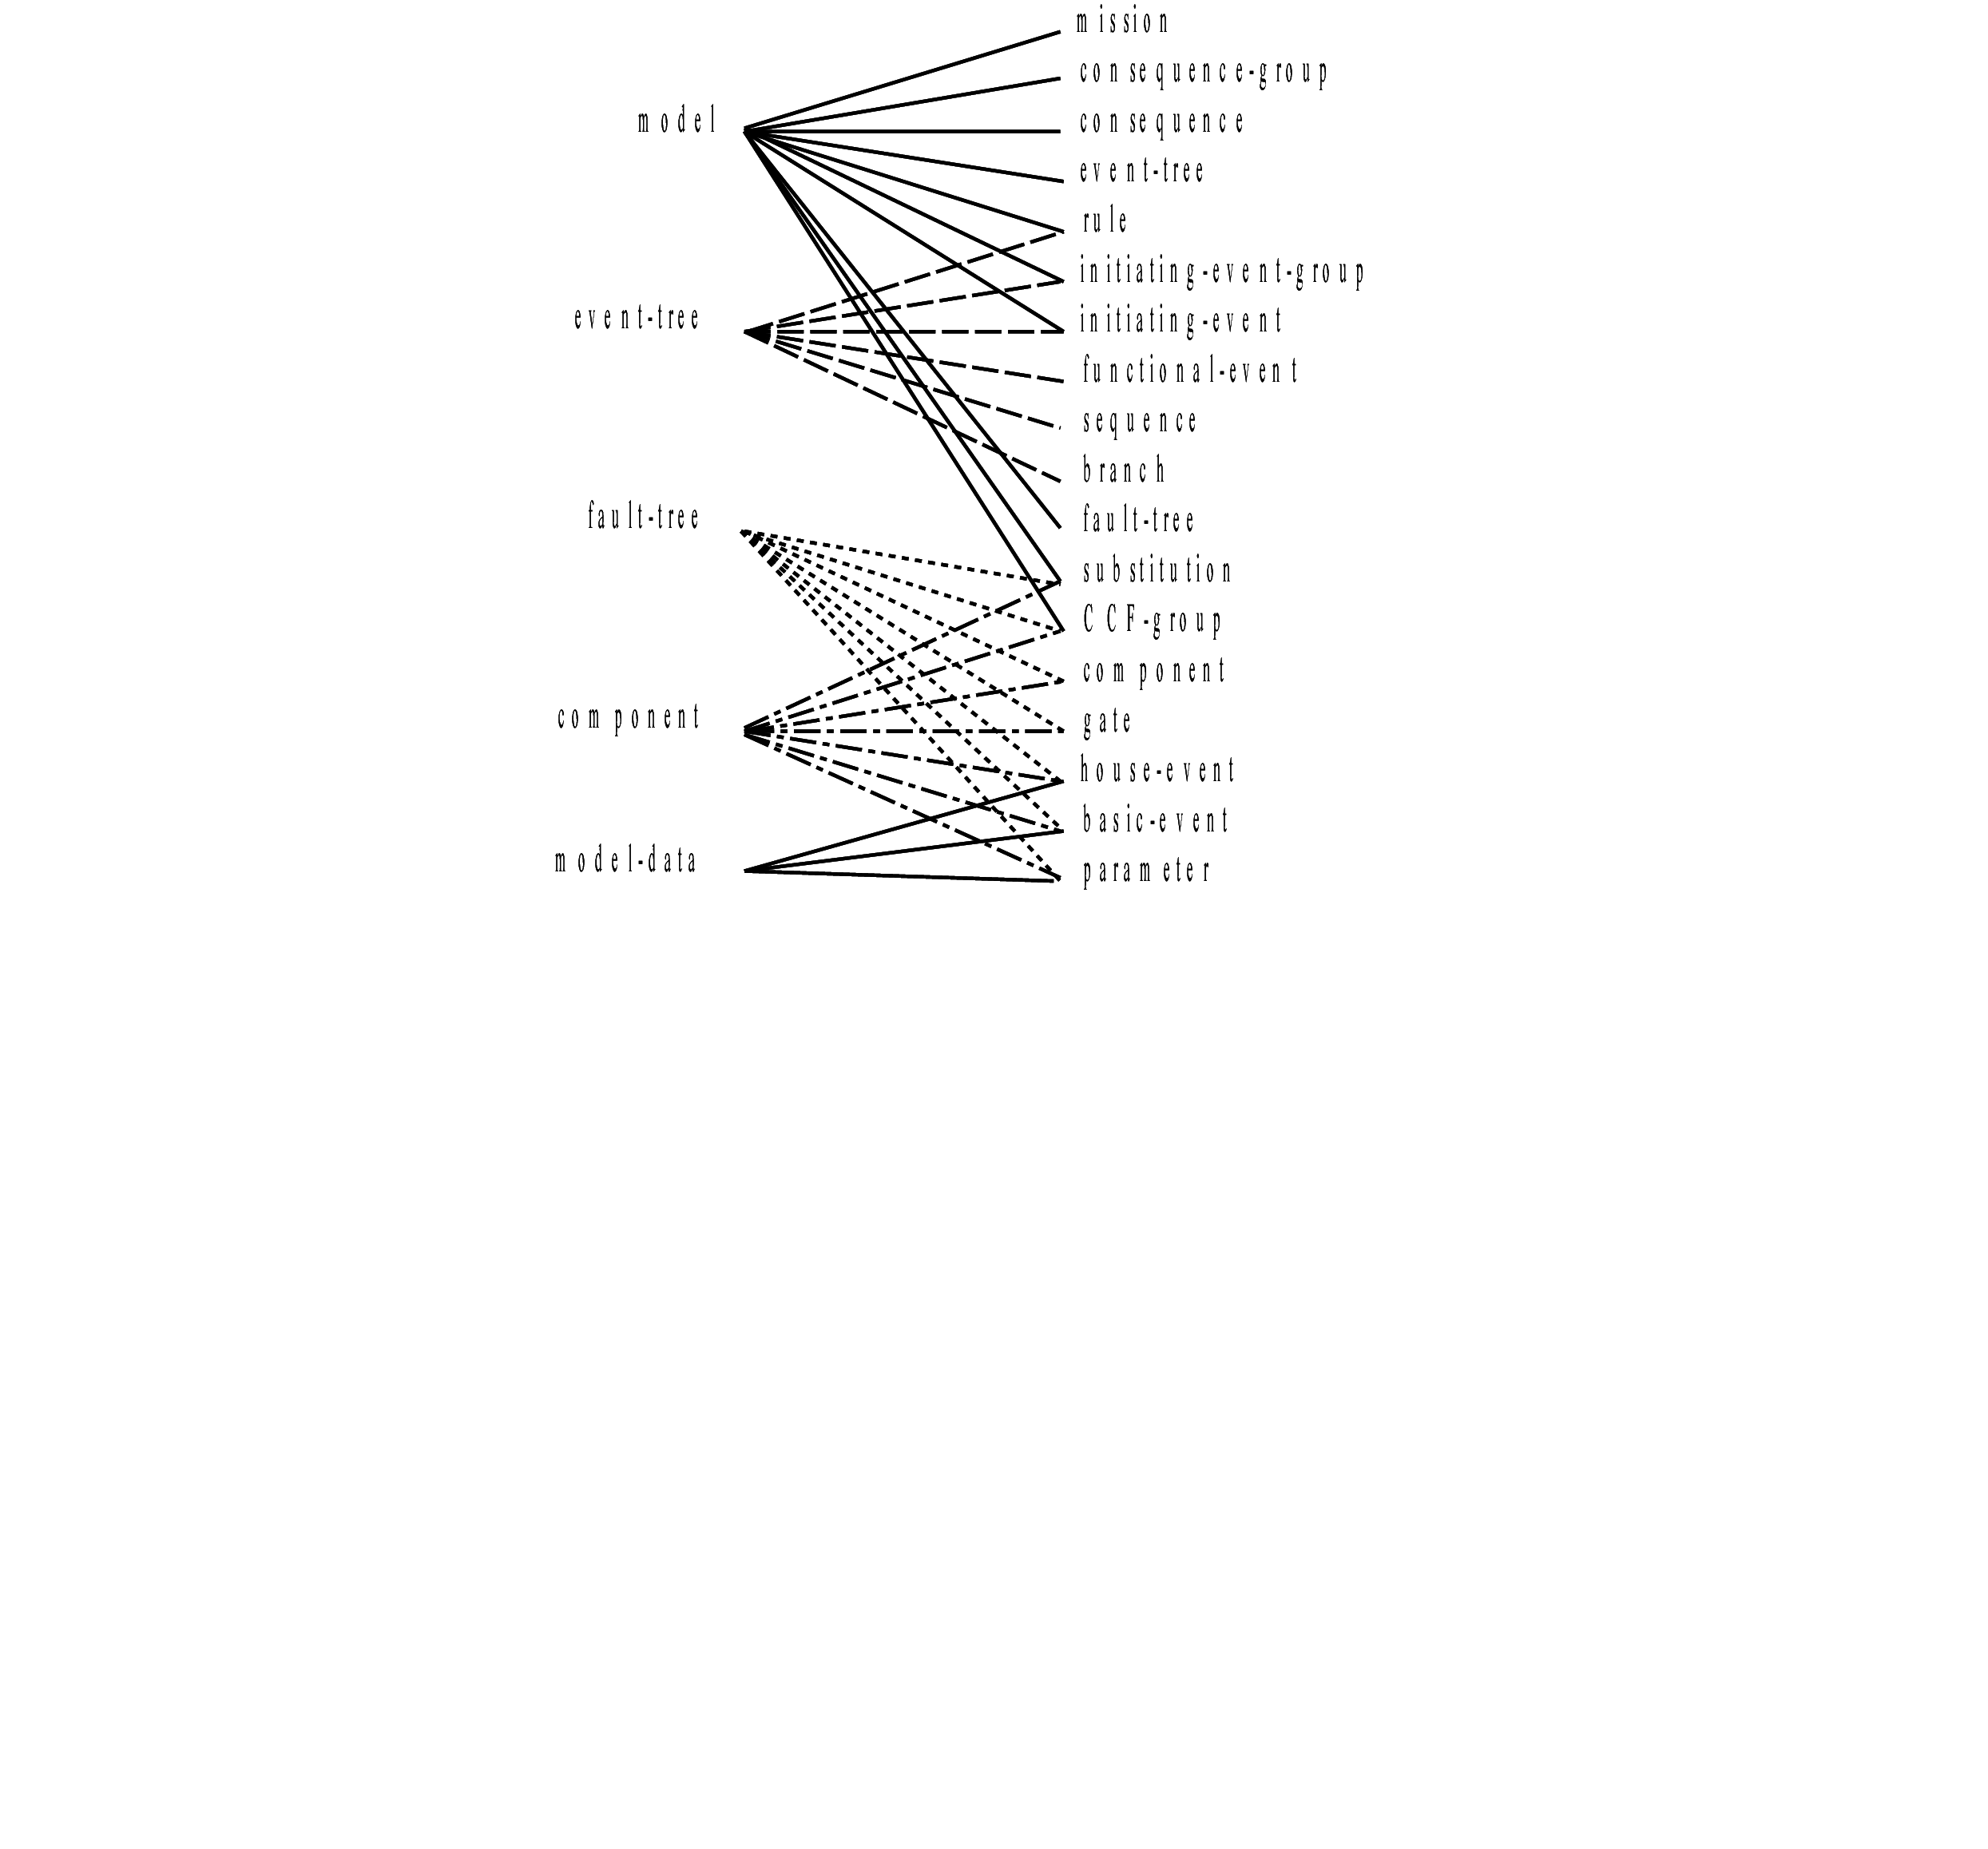
\includegraphics[width=0.9\textwidth]{./word/media/image12.png}
\caption{\label{fig:org23d0d0e}
Containers and the constructs they can define}
\end{figure}

Figure \ref{FigureVIII-32} gives the XML representation of models. This
representation just collects what has been defined so far.

\lstset{language=[LaTeX]TeX,label= ,caption={Backus-Naur form for the XML representation of containers \label{FigureVIII-32}.},captionpos=b,numbers=none}
\begin{lstlisting}
model ::=
  <?xml version="1.0" ?>
  <!DOCTYPE opsa-mef >
  <opsa-mef>
  [ label ] [ attributes ]
  (
  mission-definition
  | consequence-group-definition | consequence-definition
  | event-tree-definition
  | rule-definition
  | initiating-event-group-definition | initiating-event-definition
  | fault-tree-definition
  | substitution-definition | CCF-group-definition
  )*
  </opsa-mef>

  event-tree-definition ::=
  <define-event-tree name="identifier">
  [ label ] [ attributes ]
  functional-event-definition*
  sequence-definition*
  branch-definition*
  initial-event
  )*
  </define-event-tree>

fault-tree-definition ::=
  <define-fault-tree name="identifier">
  [ label ] [ attributes ]
  (
  substitution-definition | CCF-group-definition
  | component-definition
  | gate-definition | house-event-definition
  | basic-event-definition | parameter-definition
  )*
  </define-fault-tree>

component-definition ::=
  <define-component name="identifier">
  [ label ] [ attributes ]
  (
  substitution-definition | CCF-group-definition
  | component-definition
  | gate-definition | house-event-definition
  | basic-event-definition | parameter-definition
  )*
  </define-component>

model-data ::=
  <model-data>
  (house-event-definition | basic-event-definition |
  parameter-definition)*
  </model-data>
\end{lstlisting}

\section{Report Layer}
\label{sec:org0b286cb}


\subsection{Preliminary Discussion}
\label{sec:org5e3b1ff}

The report layer is populated with constructs to save results of
calculations. These constructs fall into two categories:

\begin{itemize}
\item Constructs to tell which software, algorithm(s) and option(s) were
used to produce the results, and

\item The results themselves.
\end{itemize}

It is almost impossible and probably not even desirable to normalize
fully the report layer. Tools are very different from one another and
produce a wide variety of results. New calculation methods are regularly
proposed. To normalize everything would lead to a huge and anyway
incomplete format. Moreover, the way results are arranged into reports
depends on the study. It is also, at least to some extent, a matter of
taste.

If the Model Exchange Format cannot give a formal structure for the
report layer, it can at least suggest a style to describe what has been
calculated and how it has been calculated. It can provide also a
check-list of what should be included as information to make results
truly exportable and importable. The existence of such report style
would be very useful for reporting tools (whether they are graphic or
textual): it would be much easier for these tools to extract the
information they need from the XML result files.

\subsection{Information about calculations}
\label{sec:orgb2b652d}

Here follows a non exhaustive list of information about how the results
have been obtained that can be relevant and other special or unique
features of the model.

\begin{itemize}
\item Software

\begin{itemize}
\item Version

\item Contact organization (editor, vendor\ldots{})

\item \ldots{}
\end{itemize}

\item Calculated quantities

\begin{itemize}
\item Name

\item Mathematic definition

\item Approximations used

\item \ldots{}
\end{itemize}

\item Calculation method(s)

\begin{itemize}
\item Name

\item Limits (e.g. number of basic events, of sequences, of cutsets)

\item Preprocessing techniques (modularization, rewritings\ldots{})

\item Handling of success terms

\item Cutoffs, if any (absolute, relative, dynamic, \ldots{})

\item Are delete terms, recovery rules or exchange events applied?

\item Extra-logical methods used

\item Secondary software necessary

\item Warning and caveats

\item Calculation time

\item \ldots{}
\end{itemize}

\item Features of the model

\begin{itemize}
\item Name

\item Number of: gates, basic events, house events, fault trees, event
trees, functional events, initiating events
\end{itemize}

\item Feedback

\begin{itemize}
\item Success or failure reports

\item \ldots{}
\end{itemize}
\end{itemize}

\subsection{Format of Results}
\label{sec:org31485c7}

PSA tools produce many different kinds of results. Some are common to
most of the tools (e.g. probability/frequency of some group of
consequences, importance factors, sensitivity analyses\ldots{}). They fall
into different categories. The following three categories are so
frequent that is it worth to normalize the way they are stored into XML
files.

\begin{itemize}
\item Minimal cutsets (and prime implicants)

\item Statistical measures (with moments)

\item Curves
\end{itemize}


\subsubsection{Minimal Cutsets}
\label{sec:org54f5059}

A first (and good) way to encode minimal cutsets consists in using the
representation of formulae defined by the Model Exchange Format.
However, it is often convenient to attach some information to each
product, which is not possible with the formulae of the Model Exchange
Format. An alternative XML representation for sums of products (sets of
minimal cutsets are a specific type of sums of products) is given Figure
\ref{FigureIX-33}. More attributes can be added to tags ``sum-of-products'' and
``product'' to carry the relevant information.


\lstset{language=[LaTeX]TeX,label= ,caption={Backus-Naur form for the XML representation of sums-of-products \label{FigureIX-33}.},captionpos=b,numbers=none}
\begin{lstlisting}
sum-of-products ::=
  <sum-of-products
  [ name="identifier" ]
  [ description="text" ]
  [ basic-events="integer" ]
  [ products="integer" ]>
  product*
  </sum-of-products>

product ::=
  <product [ order="integer" ] >
  literal*
  </product>

literal ::=
  <basic-event name="identifier" >
  | <not> 
    <basic-event name="identifier" > 
    </not>
\end{lstlisting}

\subsubsection{Statistical measures}
\label{sec:org115eb34}

Statistical measures are typically produced by sensitivity analyses.
They are the result, in general, of Monte-Carlo simulations on the
values of some parameter. Such a measure can come with moments (mean,
standard deviation), confidence ranges, error factors, quantiles\ldots{} The
XML representation for statistical measure is given Figure \ref{FigureIX-34}.


\lstset{language=[LaTeX]TeX,label= ,caption={Backus-Naur form for the XML representation of statistical measures \label{FigureIX-34}.},captionpos=b,numbers=none}
\begin{lstlisting}
measure ::=
  <measure
  [ name="identifier" ]
  [ description="text" ]
  >
  [ <mean value="float" /> ]
  [ <standard-deviation value="float" /> ]
  [ <confidence-range
  percentage="float"
  lower-bound="float"
  upper-bound="float" /> ]
  [ <error-factor percentage="float" value="float" /> ]
  [ quantiles ]
  </measure>

quantiles ::=
  <quantiles number="integer" >
  quantile+
  <quantiles/>

quantile ::=
  <quantile number="integer"
  [ mean="float" ]
  [ lower-bound="float" ]
  [ upper-bound="float" ]/>
\end{lstlisting}



\subsubsection{Curves}
\label{sec:org23e80f9}

Two or three dimensional curves are often produced in PSA studies. A
typical example is indeed to study the evolution of the system
unavailability through the time. The XML representation of curves
suggested by the Model Exchange Format is given Figure IX -35.

\lstset{language=[LaTeX]TeX,label= ,caption= ,captionpos=b,numbers=none}
\begin{lstlisting}
curve ::=
  <curve
  [ name="identifier" ]
  [ description="text" ]
  [ X-title="string" Y-title="string" [ Z-title="string" ] ]
  [ X-unit="unit" Y-unit="unit" [ Z-unit="unit" ] ]
  >
  <point X="float" Y="float" [ Z="float" ] >*
  </curve>

unit ::= seconds | hours | ...
\end{lstlisting}

Figure IX35. Backus-Naur for the XML representation of curves


\clearpage

\section{References}
\label{sec:orgd1f86de}

\textbf{Basic PSA references}

\begin{enumerate}
\item ASME RA-S-2002, "Standard for Probabilistic Risk Assessment for
Nuclear Power Plant Applications", The American Society of Mechanical
Engineers, 2002.

\item Roberts N. H., W. E. Vesely, D. F. Haasl, F. F. Goldberg, Fault Tree
Handbook, NUREG-0492, US NRC, Washington, 1981.

\item W. Vesely, J. Dugan, J. Fragola, J. Minarick, J. Railsback, Fault
Tree Handbook with Aerospace Applications, National Aeronautics and
Space Administration, NASA, 2002

\item Regulatory Guide 1200, An Approach for Determining the Technical
Adequacy of Probabilistic Risk Assessment Results for Risk-Informed
Activities, US NRC, 2004.

\item US NRC Regulatory Guide 1.174 "An Approach for Using Probabilistic
Risk Assessment in Risk-Informed Decisions on Plant-Specific Changes
to the Licensing Basis", Revision 1, US NRC, 2002.

\item 
\end{enumerate}

\textbf{Difficulties with PSA}

\begin{enumerate}
\item Čepin M., Analysis of Truncation Limit in Probabilistic Safety
Assessment, Reliability Engineering and System Safety, 2005, Vol. 87
(3), pp. 395-403.

\item S. Epstein and A. Rauzy, Can we trust PRA?, Reliability Engineering \&
System Safety, Volume 88, Issue 3, June 2005, Pages 195-205
\end{enumerate}



\textbf{Novel approaches}

\begin{enumerate}
\item Antoine Rauzy, New algorithms for fault trees analysis, Reliability
Engineering \& System Safety, Volume 40, Issue 3, 1993, Pages 203-211

\item Antoine Rauzy and Yves Dutuit, Exact and truncated computations of
prime implicants of coherent and non-coherent fault trees within
Aralia, Reliability Engineering \& System Safety, Volume 58, Issue 2,
November 1997, Pages 127-144

\item Poul Frederick Williams, Macha Nikolskaïa and Antoine Rauzy,
Bypassing BDD construction for reliability analysis, Information
Processing Letters, Volume 75, Issues 1-2, 31 July 2000, Pages 85-89

\item Y. Dutuit and A. Rauzy, Approximate estimation of system reliability
via fault trees, Reliability Engineering \& System Safety, Volume 87,
Issue 2, February 2005, Pages 163-172

\item Čepin M., B. Mavko, A Dynamic Fault Tree, Reliability Engineering and
System Safety, 2002, Vol. 75, No. 1, pp. 83-91.

\item Albert F. Myers and Antoine Rauzy, Assessment of redundant systems
with imperfect coverage by means of binary decision diagrams,
Reliability Engineering \& System Safety, Volume 93, Issue 7, July
2008, Pages 1025-1035
\end{enumerate}



\clearpage
\appendix

\section{Extended Backus-Naur Form}
\label{sec:org094afc7}

\emph{The following presentation is inspired from the article about the
Backus-Naur form in Wikipedia.}

The Backus--Naur form (also known as BNF, the Backus--Naur formalism or
Backus normal form) is a meta-syntax used to express context-free
grammars: that is, a formal way to describe formal languages. BNF is
widely used as a notation for the grammars of computer programming
languages. Most textbooks for programming language theory and/or
semantics document the programming language in BNF.

A BNF specification is a set of derivation rules, written as

\lstset{language=[LaTeX]TeX,label= ,caption= ,captionpos=b,numbers=none}
\begin{lstlisting}
symbol ::= < /expression/ with symbols>
\end{lstlisting}

where \emph{symbol} is a nonterminal, and the expression consists of
sequences of symbols and/or sequences separated by the vertical bar,
'|', indicating a choice, the whole being a possible substitution for
the symbol on the left. Symbols that never appear on a left side are
terminals.

As an example, consider this possible BNF for a U.S. postal address:

\lstset{language=[LaTeX]TeX,label= ,caption= ,captionpos=b,numbers=none}
\begin{lstlisting}
postal-address ::= name-part street-address zip-part
name-part ::=
  personal-part last-name [ jr-part ] EOL 
  | personal-part name-part EOL

personal-part ::= first-name | initial .
jr-part ::= Jr | Sr | dynastic-number
street-address ::= [ apartement-number ] house-number street-name EOL
zip-part ::= town-name , state-code ZIP-code EOL
\end{lstlisting}

This translates into English as:

\begin{itemize}
\item A postal address consists of a name-part, followed by a
street-address part, followed by a zip-code part.

\item A name-part consists of either: a personal-part followed by a last
name followed by an optional "jr-part" (Jr., Sr., or dynastic number)
and end-of-line, or a personal part followed by a name part (this
rule illustrates the use of recursion in BNFs, covering the case of
people who use multiple first and middle names and/or initials).

\item A personal-part consists of either a first name or an initial
followed by a dot.

\item A street address consists of an optional apartment specifier,
followed by a house number, followed by a street name, followed by an
end-of-line.

\item A zip-part consists of a town-name, followed by a comma, followed by
a state code, followed by a ZIP-code followed by an end-of-line.
\end{itemize}

Note that many things (such as the format of a first-name, apartment
specifier, or ZIP-code) are left unspecified here. If necessary, they
may be described using additional BNF rules.

There are many variants and extensions of BNF, generally either for the
sake of simplicity and succinctness, or to adapt it to a specific
application. One common feature of many variants is the use of regular
expressions repetition operators such as * and +. The Extended
Backus-Naur form we shall use is as follows.

\begin{itemize}
\item Non terminal symbols are \emph{italicized}, terminal symbols are written
in regular font.

\item Optional items enclosed in square brackets. E.g. [ \emph{item-x} ].

\item Items repeating 1 or more times are followed by a '+'.

\item Items repeating 0 or more times are followed by a '*'.

\item Items repeating k times are enclosed in square brackets followed by
‘:k'. E.g. [ \emph{item-x} ]:3.

\item Items repeating n or more times are followed by 'n'.

\item Where items need to be grouped they are enclosed in simple
parenthesis.

\item Comments start with a ‘\#' and spread until the end of the line
\end{itemize}

\section{DTD of the Open-PSA Model Exchange Format}
\label{sec:org05b6144}


\lstset{language=XML,label= ,caption= ,captionpos=b,numbers=none}
\begin{lstlisting}
<!------------------------------------------------------------------>

<!-- I. Report/Calculation Layer -->

<!------------------------------------------------------------------>

<!------------------------------------------------------------------>

<!-- I.1. Models -->

<!------------------------------------------------------------------>

<!ELEMENT opsa-mef

(label?, attributes?,

(

define-event-tree

| define-alignment

| define-consequence-group | define-consequence

| define-rule

| define-initiating-event-group | define-initiating-event

| define-fault-tree

| define-substitution

| define-CCF-group

| include

)*

)

>

<!ELEMENT label (#PCDATA)>

<!ELEMENT attributes attribute* >

<!ELEMENT attribute EMPTY>

<!ATTLIST attribute

name CDATA #REQUIRED value CDATA #REQUIRED type CDATA #IMPLIED >

<!ELEMENT include EMPTY>

<!ATTLIST include file CDATA #REQUIRED >

<!------------------------------------------------------------------>

<!-- I.2. Consequences, Consequence Groups -->

<!------------------------------------------------------------------>

<!ELEMENT define-consequence (label?, attributes?, initiating-event,
sequence) >

<!ATTLIST define-consequence name CDATA #REQUIRED >

<!ELEMENT define-consequence-group

(label?, attributes?, (consequence | consequence-group)* )

>

<!ATTLIST define-consequence-group name CDATA #REQUIRED >

<!ELEMENT consequence EMPTY>

<!ATTLIST consequence name CDATA #REQUIRED >

<!ELEMENT consequence-group EMPTY>

<!ATTLIST consequence-group name CDATA #REQUIRED >

<!------------------------------------------------------------------>

<!-- I.3. Missions, Phases -->

<!------------------------------------------------------------------>

<!ELEMENT define-alignment (label?, attributes?, instruction* ) >

<!ATTLIST define-alignment name CDATA #REQUIRED >

<!------------------------------------------------------------------>

<!-- II. Event Tree Layer -->

<!------------------------------------------------------------------>

<!------------------------------------------------------------------>

<!-- II.1. Initiating events, Initiating event Groups -->

<!------------------------------------------------------------------>

<!ENTITY % collected-item '(basic-event | gate | parameter)' >

<!ELEMENT define-initiating-event

(label?, attributes?,

(collected-item | consequence | consequence-group)* )

>

<!ATTLIST define-initiating-event name CDATA #REQUIRED >

<!ELEMENT define-initiating-event-group

(label?, attributes?, (initiating-event | initiating-event-group)* )

>

<!ATTLIST define-initiating-event-group name CDATA #REQUIRED >

<!ELEMENT initiating-event EMPTY>

<!ATTLIST initiating-event name CDATA #REQUIRED event-tree CDATA
#IMPLIED >

<!ELEMENT initiating-event-group EMPTY>

<!ATTLIST initiating-event-group

name CDATA #REQUIRED event-tree CDATA #IMPLIED >

<!------------------------------------------------------------------>

<!-- II.2. Event Trees -->

<!------------------------------------------------------------------>

<!ENTITY % end-state '(sequence | branch)'>

<!ENTITY % branch '(instruction* (fork | end-state))'>

<!ELEMENT define-event-tree

(label?, attributes?,

define-functional-event*,

define-sequence*,

define-branch*

initial-state)

>

<!ATTLIST define-event-tree name CDATA #REQUIRED >

<!ELEMENT define-functional-event (label?, attributes?) >

<!ATTLIST define-functional-event name CDATA #REQUIRED >

<!ELEMENT define-sequence (label?, attributes?, instruction*) >

<!ATTLIST define-sequence name CDATA #REQUIRED >

<!ELEMENT define-branch (label?, attributes?, branch) >

<!ATTLIST define-branch name CDATA #REQUIRED >

<!ELEMENT fork (path)+>

<!ATTLIST fork functional-event CDATA #REQUIRED >

<!ELEMENT path (branch)+ >

<!ATTLIST path state CDATA #REQUIRED >

<!ELEMENT initial-state branch>

<!------------------------------------------------------------------>

<!-- II.3. Instructions, Rules -->

<!------------------------------------------------------------------>

<!ENTITY % set

'(set-gate | set-house-event | set-basic-event | set-parameter)' >

<!ENTITY % collect '(collect-formula | collect-expression)' >

<!ENTITY % instruction '(set | collect | if | block | rule |
event-tree)'>

<!ENTITY % directions '(forward | backward | both)'>

<!ELEMENT set-gate formula >

<!ATTLIST set-gate name CDATA #REQUIRED direction directions #IMPLIED >

<!ELEMENT set-house-event Constant >

<!ATTLIST set-house-event name CDATA #REQUIRED direction directions
#IMPLIED >

<!ELEMENT set-basic-event expression >

<!ATTLIST set-basic-event name CDATA #REQUIRED direction directions
#IMPLIED >

<!ELEMENT set-parameter expression >

<!ATTLIST set-parameter name CDATA #REQUIRED direction directions
#IMPLIED >

<!ELEMENT if (expression, instruction, instruction?) >

<!ELEMENT collect-formula formula>

<!ELEMENT collect-expression expression>

<!ELEMENT block instruction* >

<!ELEMENT event-tree EMPTY >

<!ATTLIST set-parameter name CDATA #REQUIRED >

<!ELEMENT rule EMPTY >

<!ATTLIST rule name CDATA #REQUIRED >

<!------------------------------------------------------------------>

<!-- III. Meta-Logical Layer -->

<!------------------------------------------------------------------>

<!------------------------------------------------------------------>

<!-- III.1. CCF-Groups -->

<!------------------------------------------------------------------>

<!ELEMENT define-CCF-group

(label?, attributes?, members, distribution, factors) >

<!ATTLIST define-CCF-group

name CDATA #REQUIRED

model (beta-factor | MGL | alpha-factor | phi-factor) #REQUIRED >

<!ELEMENT members basic-event+ >

<!ELEMENT factors factor+ >

<!ELEMENT factor expression >

<!ATTLIST factor level CDATA #REQUIRED >

<!------------------------------------------------------------------>

<!-- III.2. Substitutions -->

<!------------------------------------------------------------------>

<!ELEMENT distribution expression >

<!ELEMENT define-substitution

(label?, attributes?, hypothesis, source?, target) >

<!ATTLIST define-substitution name CDATA #IMPLIED type CDATA #IMPLIED >

<!ELEMENT hypothesis Boolean-formula >

<!ELEMENT source basic-event+ >

<!ELEMENT target (basic-event+ | Boolean-formula) >

<!------------------------------------------------------------------>

<!-- IV. Fault Tree Layer -->

<!------------------------------------------------------------------>

<!------------------------------------------------------------------>

<!-- IV.1. Definitions of Fault Trees & Components -->

<!------------------------------------------------------------------>

<!ELEMENT define-fault-tree

(label?, attributes?,

(

define-substitution | define-CCF-group

| define-component

| define-gate | define-house-event

| define-basic-event | define-parameter

| include

)*

>

<!ATTLIST define-fault-tree name CDATA #IMPLIED >

<!ELEMENT define-component

(label?, attributes?,

(

define-substitution | define-CCF-group

| define-component

| define-gate | define-house-event

| define-basic-event | define-parameter

| include

)*

>

<!ATTLIST define-component

name CDATA #REQUIRED

role (private | public) #IMPLIED

>

<!ELEMENT model-data

( define-house-event | define-basic-event | define-parameter | include
)*

>

<!------------------------------------------------------------------>

<!-- IV.2. Definitions of Gates, House Events & Basic Events -->

<!------------------------------------------------------------------>

<!ELEMENT define-gate (label?, attributes?, formula) >

<!ATTLIST define-component

name CDATA #REQUIRED

role (private | public) #IMPLIED

>

<!ELEMENT define-house-event (label?, attributes?, Constant? ) >

<!ATTLIST define-house-event

name CDATA #REQUIRED

role (private | public) #IMPLIED

>

<!ELEMENT define-basic-event (label?, attributes?, expression?) >

<!ATTLIST define-basic-event

name CDATA #REQUIRED

role (private | public) #IMPLIED

>

<!------------------------------------------------------------------>

<!-- IV.3. Formulae -->

<!------------------------------------------------------------------>

<!ELEMENT formula (

gate | house-event | basic-event | Constant

| and | or | not | xor | iff | nand | nor | atleast | cardinality ) >

<!ELEMENT gate EMPTY>

<!ATTLIST gate name CDATA #REQUIRED>

<!ELEMENT house-event EMPTY>

<!ATTLIST house-event name CDATA #REQUIRED>

<!ELEMENT basic-event EMPTY>

<!ATTLIST basic-event name CDATA #REQUIRED>

<!ELEMENT and formula+ >

<!ELEMENT or formula+ >

<!ELEMENT not formula >

<!ELEMENT xor formula+ >

<!ELEMENT iff formula+ >

<!ELEMENT nand formula+ >

<!ELEMENT nor formula+ >

<!ELEMENT atleast formula+ >

<!ATTLIST atleast min CDATA #REQUIRED>

<!ELEMENT cardinality formula+ >

<!ATTLIST cardinality min CDATA #REQUIRED max CDATA #REQUIRED>

<!ELEMENT imply formula formula >

<!ELEMENT constant EMPTY >

<!ATTLIST constant value (true | false) #REQUIRED>

<!------------------------------------------------------------------>

<!-- V. Stochastic Layer -->

<!------------------------------------------------------------------>

<!------------------------------------------------------------------>

<!-- V.1. Definition of Parameters -->

<!------------------------------------------------------------------>

<!ENTITY % units

'( bool | int | float | hours | hours-1 | years | years-1

| fit | demands ) ' >

<!ELEMENT define-parameter (label?, attributes?, expression?) >

<!ATTLIST define-parameter

name CDATA #REQUIRED

role (private | public) #IMPLIED

unit units #IMPLIED >

<!------------------------------------------------------------------>

<!-- V.2. Expressions -->

<!------------------------------------------------------------------>

<!------------------------------------------------------------------>

<!-- V.2.1. Entities -->

<!------------------------------------------------------------------>

<!ENTITY % value

'( bool | int | float )' >

<!ENTITY % numerical-operation

'( neg | add | sub | mul | div | pi | abs | acos | asin | atan | cos

| cosh | exp | log | log10 | mod | pow | sin | sinh | tan | tanh

| sqrt | ceil | floor | min | max | mean )' >

<!ENTITY % Boolean-operation

'( not | and | or | eq | df | lt | gt | leq | geq )' >

<!ENTITY % conditional-operation '( ite | switch )' >

<!ENTITY % operation

'( numerical-operation | Boolean-operation | conditional-operation)' >

<!ENTITY % built-in

'( exponential | GLM | Weibull | periodic-test | extern-function )' >

<!ENTITY % random-deviate

'( uniform-deviate | normal-deviate | lognormal-deviate | gamma-deviate

| beta-deviate | histogram )' >

<!ENTITY % test-event '( test-initiating-event | test-functional-event)'
>

<!ENTITY % expression

'( value | parameter | system-mission-time | operation| built-in

| random-deviate | test-event )' >

<!------------------------------------------------------------------>

<!-- V.2.2. Constants, Parameters -->

<!------------------------------------------------------------------>

<!ELEMENT bool EMPTY >

<!ATTLIST value (true | false) #REQUIRED>

<!ELEMENT int EMPTY >

<!ATTLIST value CDATA #REQUIRED>

<!ELEMENT float EMPTY >

<!ATTLIST value CDATA #REQUIRED>

<!ELEMENT system-mission-time EMPTY >

<!ATTLIST unit units #IMPLIED >

<!ELEMENT parameter EMPTY >

<!ATTLIST name CDATA #REQUIRED >

<!------------------------------------------------------------------>

<!-- V.2.3. Numerical Expressions -->

<!------------------------------------------------------------------>

<!ELEMENT neg expression >

<!ELEMENT add expression+ >

<!ELEMENT sub expression+ >

<!ELEMENT mul expression+ >

<!ELEMENT div expression+ >

<!ELEMENT pi EMPTY >

<!ELEMENT abs expression >

<!ELEMENT acos expression >

<!ELEMENT asin expression >

<!ELEMENT atan expression >

<!ELEMENT cos expression >

<!ELEMENT cosh expression >

<!ELEMENT exp expression >

<!ELEMENT log expression >

<!ELEMENT log10 expression >

<!ELEMENT mod (expression, expression) >

<!ELEMENT pow (expression, expression) >

<!ELEMENT sin expression >

<!ELEMENT sinh expression >

<!ELEMENT tan expression >

<!ELEMENT tanh expression >

<!ELEMENT sqrt expression >

<!ELEMENT ceil expression >

<!ELEMENT floor expression >

<!ELEMENT min expression+ >

<!ELEMENT max expression+>

<!ELEMENT mean expression+ >

<!------------------------------------------------------------------>

<!-- V.2.4. Boolean Expressions -->

<!------------------------------------------------------------------>

<!ELEMENT not expression >

<!ELEMENT and expression+ >

<!ELEMENT or expression+ >

<!ELEMENT eq (expression, expression) >

<!ELEMENT df (expression, expression) >

<!ELEMENT lt (expression, expression) >

<!ELEMENT gt (expression, expression) >

<!ELEMENT leq (expression, expression) >

<!ELEMENT geq (expression, expression) >

<!------------------------------------------------------------------>

<!-- V.2.5. Conditional Expressions -->

<!------------------------------------------------------------------>

<!ELEMENT ite (expression, expression, expression) >

<!ELEMENT switch (case*, expression) >

<!ELEMENT case (expression, expression)>

<!------------------------------------------------------------------>

<!-- V.2.6. Built-ins -->

<!------------------------------------------------------------------>

<!ELEMENT exponential (expression, expression) >

<!ELEMENT GLM (expression, expression, expression, expression) >

<!ELEMENT Weibull (expression, expression, expression) >

<!ELEMENT periodic-test expression+ >

<!ELEMENT extern-function expression* >

<!ATTLIST extern-function name CDATA #REQUIRED>

<!------------------------------------------------------------------>

<!-- V.2.7. Random-Deviates -->

<!------------------------------------------------------------------>

<!ELEMENT uniform-deviate (expression, expression) >

<!ELEMENT normal-deviate (expression, expression) >

<!ELEMENT lognormal-deviate (expression, expression, expression) >

<!ELEMENT gamma-deviate (expression, expression) >

<!ELEMENT beta-deviate (expression, expression)>

<!ELEMENT histogram (expression, bin+) >

<!ELEMENT bin (expression, expression) >

<!------------------------------------------------------------------>

<!-- V.2.8. Test-Events -->

<!------------------------------------------------------------------>

<!ELEMENT test-initiating-event >

<!ATTLIST test-initiating-event name CDATA #REQUIRED >

<!ELEMENT test-functional-event >

<!ATTLIST test-functional-event name CDATA #REQUIRED state CDATA
#REQUIRED >
\end{lstlisting}

\section{Backus-Naur form for the Open-PSA Model Exchange Format}
\label{sec:orgf1d5a66}


\subsection{Models}
\label{sec:orgb7f6d56}

\lstset{language=XML,label= ,caption= ,captionpos=b,numbers=none}
\begin{lstlisting}
model ::=
  <?xml version="1.0" ?>
  <!DOCTYPE opsa-mef >
  <opsa-mef [ name="identifier" ] >
  [ label ] [ attributes ]
  (
  event-tree-definition
  | alignment-definition
  | consequence-group-definition | consequence-definition
  | rule-definition
  | initiating-event-group-definition | initiating-event-definition
  | fault-tree-definition
  | substitution-definition
  | CCF-group-definition
  | include-directive
  )*
  </opsa-mef>
label :=
  <label> any text </label>
  attributes ::=
  <attributes> attribute+ </attributes>
attribute ::=
  <attribute name="identifier" value="string" [ type="string" ]  />
  include-directive ::=
  <include file="string" />
\end{lstlisting}


\subsection{Consequence, Consequence Groups, Alignments}
\label{sec:org2d1e0fb}


\lstset{language=[LaTeX]TeX,label= ,caption= ,captionpos=b,numbers=none}
\begin{lstlisting}
consequence-definition ::=
  <define-consequence name="identifier">
  [ label ] [ attributes ]
  <initiating-event name="identifier"/>
  <sequence name="identifier" />
  </define-consequence>

consequence-group-definition ::=
  <define-consequence-group name="identifier" >
  [ label ] [ attributes ]
  consequence | consequence-group
  </define-consequence-group>
consequence ::=
  <consequence name="identifier" />

consequence-group ::=
  <consequence-group name="identifier" />

alignment-definition ::=
  <define-alignment name="identifier" time-fraction="float" >
  [ label ] [ attributes ]
  instruction*
  </define-alignment>
\end{lstlisting}

\subsection{Initiating events, Initiating event Groups}
\label{sec:org198fe6d}

\lstset{language=[LaTeX]TeX,label= ,caption= ,captionpos=b,numbers=none}
\begin{lstlisting}
initiating-event-definition ::=
  <define-initiating-event name="identifier" [event-tree="identifier"]>
  [ label ] [ attributes ]
  [ collected-item | consequence | consequence-group ]
  </define-initiating-event>

initiating-event-group-definition ::=
  <define-initiating-event-group name="identifier"
  [event-tree="identifier"] >
  [ label ] [ attributes ]
  initiating-event+
  </define-initiating-event-group>
  initiating-event ::=
  <initiating-event name="identifier" >
    |<initiating-event-group name="identifier" >

collected-item ::=
  <basic-event name="identifier" >
  | <gate name="identifier" >
  | <parameter name="identifier" >
\end{lstlisting}

\subsection{Event Trees}
\label{sec:org3fc964b}


\lstset{language=[LaTeX]TeX,label= ,caption= ,captionpos=b,numbers=none}
\begin{lstlisting}
event-tree-definition ::=
  <define-event-tree name="identifier">
  [ label ] [ attributes ]
  functional-event-definition*
  sequence-definition*
  branch-definition*
  initial-state
  </define-event-tree>

functional-event-definition ::=
  <define-functional-event name="identifier" >
  [ label ]
  [ attributes ]
  </define-functional-event>

sequence-definition ::=
  <define-sequence name="identifier" >
  [ label ]
  [ attributes ]
  instruction+
  </define-sequence>

branch-definition ::=
  <define-branch name="identifier" >
  [ label ]
  [ attributes ]
  branch
  </define-branch>

branch ::= instruction* (fork | end-state)
fork ::= <fork functional-event="identifier"> path+ <fork>
path ::= <path state="identifier" > branch <path>
end-state ::=
  <sequence name="identifier" >
  | <branch name="identifier" >

initial-state ::=
<initial-state> branch </initial-state>
\end{lstlisting}

\subsection{Instructions, Rules}
\label{sec:orga2768e6}


\lstset{language=[LaTeX]TeX,label= ,caption= ,captionpos=b,numbers=none}
\begin{lstlisting}
instruction ::= set | collect | if-then-else | block | rule | link

set ::= set-gate | set-house-event | set-basic-event | set-parameter

set-gate ::=
  <set-gate name="identifier" [ direction="direction" ] >
  formula
  </set-gate>

set-house-event ::=
  <set-house-event name="identifier" [ direction="direction" ] >
  Boolean-constant
  </set-house-event>

set-basic-event ::=
  <set-basic-event name="identifier" [ direction="direction" ] >
  expression
  </set-basic-event>

set-parameter ::=
  <set-parameter name="identifier" [ direction="direction" ] >
  expression
  </set-parameter>

direction ::= forward | backward | both
if-then-else ::=
  <if> expression instruction [ instruction ] </if>

collect ::= collect-formula | collect-expression

collect-formula ::= <collect-formula> formula </collect-formula>

collect-expression ::= <collect-expression> expression </collect-expression>
block ::= <block> instruction* <block>
rule ::= <rule name="identifier" >
link ::= <event-tree name="name" >
rule-definition ::=
  <define-rule name="identifier" >
  [ label ] [ attributes ]
  instruction+
  </define-rule>
\end{lstlisting}

\subsection{CCF-groups, Substitutions}
\label{sec:org9740434}


\lstset{language=[LaTeX]TeX,label= ,caption= ,captionpos=b,numbers=none}
\begin{lstlisting}
CCF-group-definition ::=
  <define-CCF-group name="identifier" model="CCF-model" >
  [ label ]
  [ attributes ]
  members
  distribution
  factors
</define-CCF-group>
members ::=
  <members>
  <basic-event name="identifier" >+
  </members>

factors ::=
  <factors> factor+ </factors>
  | factor

factor ::=
  <factor [ level="integer" ] >
  expression
  <factor>

distribution ::=
  <distribution >
  expression
  <distribution>

CCF-model ::= beta-factor | MGL | alpha-factor | phi-factor

substitution-definition ::=
  <define-substitution [ name="identifier" ] [ type="identifier" >
  [ label ]
  [ attributes ]
  <hypothesis> Boolean-formula <hypothesis>
  [ <source> basic-event+ <source> ]
  <target> basic-event+ | Boolean-constant <target>
  <define-substitution >
\end{lstlisting}

\subsection{Fault Trees, Components}
\label{sec:orga11a831}


\lstset{language=[LaTeX]TeX,label= ,caption= ,captionpos=b,numbers=none}
\begin{lstlisting}
/fault-tree-definition/ ::=
  <define-fault-tree name="identifier">
  [ label ]
  [ attributes ]
  (
  substitution-definition | /CCF-group-definition/
  | /component-definition/
  | /gate-definition/ | /house-event-definition/
  | /basic-event-definition/ | /parameter-definition/
  | /include-directive/
  )*
  </define-fault-tree>


component-definition ::=
  <define-component name="/identifier/">
  [ /label/ ]
  [ /attributes/ ]
  (
  substitution-definition | /CCF-group-definition/
  | /component-definition/
  | /gate-definition/ | /house-event-definition/
  | /basic-event-definition/ | /parameter-definition/
  | /include-directive/
  )*
  </define-component>

model-data ::=
  <model-data>
  ( /house-event-definition/ | /basic-event-definition/ |
  parameter-definition )*
  </model-data>

event-definition ::=
  gate-definition
  | /house-event-definition/
  | /basic-event-definition/

gate-definition ::=
  <define-gate name="/identifier/" [ role="private|public" ] >
  [ /label/ ]
  [ /attributes/ ]
  /formula/
  </define-gate>

house-event-definition ::=
  <define-house-event name="/identifier/" [ role="private|public" ] >
  [ /label/ ]
  [ /attributes/ ]
  [ /Boolean-constant/ ]
  </define-house-event>
\end{lstlisting}

\subsection{Formulae}
\label{sec:org4ab34fb}



\lstset{language=[LaTeX]TeX,label= ,caption= ,captionpos=b,numbers=none}
\begin{lstlisting}
/formula/ ::=
/event/
| /Boolean-constant/
| <and> formula+ <and>
| <or> formula+ <or>
| <not> /formula/ <not>
| <xor> formula+ <xor>
| <iff> formula+ <iff>
| <nand> formula+ <nand>
| <nor> formula+ <nor>
| <atleast min="/integer/" > formula+ <atleast>
| <cardinality min="/integer/" max="/integer/" > formula+
<cardinality>
| <imply> /formula/ /formula/ <imply>
/event/ ::=
<event name="/identifier/" [ type="/event-type/" ] >
| <gate name="/identifier/" >
| <house-event name="/identifier/" >
| <basic-event name="/identifier/" >
/event-type/ ::= gate | basic-event | house-event
/Boolean-constant/ ::= <constant value="/Boolean-value/" >
/Boolean-value/ ::= true | false
\end{lstlisting}

\subsection{Basic Events, Parameters}
\label{sec:org795fe47}

\lstset{language=[LaTeX]TeX,label= ,caption= ,captionpos=b,numbers=none}
\begin{lstlisting}
/basic-event-definition/ ::=
  <define-basic-event name="/identifier/" [ role="private|public" ] >
  [ /label/ ]
  [ /attributes/ ]
  [ /expression/ ]
  </declare>

/parameter-definition/ ::=
  <define-parameter name="/identifier/"
  [ role="private|public" ] [ unit="/unit/" ]>
  [ /label/ ]
  [ /attributes/ ]
  /expression/
  </define-parameter>

/unit/ ::= bool | int | float | hours | hours-1 | years | years-1 | demands | fit
\end{lstlisting}

\subsection{Expressions}
\label{sec:orga72b1df}

\lstset{language=[LaTeX]TeX,label= ,caption= ,captionpos=b,numbers=none}
\begin{lstlisting}
expression ::=
  constant | parameter | operation | built-in | random-deviate | test-event
constant ::=
  <bool value="Boolean-value" />
  | <int value="integer" />
  | <float value="float" />

parameter ::=
  <parameter name="identifier" [ type="value-type" ] />
  | <system-mission-time [ unit="unit" ] />

operation ::=
 numerical-operation | Boolean-operation | conditional-operation

numerical-operation ::=
   <neg> expression </neg>
  | <add> expression+ </add>
  | <sub> expression+ </sub>
  | <mul> expression+ </mul>
  | <div> expression+ </div>
  | <pi />
  | <abs> expression </abs>
  | <acos> expression </acos>
  | <asin> expression </asin>
  | <atan> expression </atan>
  | <cos> expression </cos>
  | <cosh> expression </cosh>
  | <exp> expression </exp>
  | <log> expression </log>
  | <log10> expression </log10>
  | <mod> expression expression </mod>
  | <pow> expression expression </pow>
  | <sin> expression </sin>
  | <sinh> expression </sinh>
  | <tan> expression </tan>
  | <tanh> expression </tanh>
  | <sqrt> expression </sqrt>
  | <ceil> expression </ceil>
  | <floor> expression </floor>
  | <min> expression+ </min>
  | <max> expression+ </max>
  | <mean> expression+ </mean>

Boolean-operation ::=
  <not> expression </not>
  | <and> expression+ </and>
  | <or> expression+ </or>
  | <eq> expression expression </eq>
  | <df> expression expression </df>
  | <lt> expression expression </lt>
  | <gt> expression expression </gt>
  | <leq> expression expression </leq>
  | <geq> expression expression </geq>

conditional-operation ::=
  if-then-else-operation | switch-operation

if-then-else-operation ::=
   <ite> expression expression expression </ite>

switch-operation ::=
  <switch>
  case-operation *
  expression
  </switch>

case-operation ::=
 <case> expression expression </case>

built-in ::=
   <exponential> [ expression ]:2 </exponential>
  | <GLM> [ expression ]:4 </GLM>
  | <Weibull> [ expression ]:3 </Weibull>
  | <periodic-test> [ expression ]:11 </periodic-test>
  | <periodic-test> [ expression ]:5 </periodic-test>
  | <periodic-test> [ expression ]:4 </periodic-test>
  | <extern-function name="name" > expression* </extern-function>
random-deviate ::=
   <uniform-deviate> [ expression ]:2 </uniform-deviate>
  | <normal-deviate> [ expression ]:2 </normal-deviate>
  | <lognormal-deviate> [ expression ]:3 </lognormal-deviate>
  | <gamma-deviate> [ expression ]:2 </gamma-deviate>
  | <beta-deviate> [ expression ]:2 </beta-deviate>
  | histogram

histogram ::=
   <histogram > expression bin+ </histogram>
bin ::=
  <bin> expression expression </bin>

test-event ::=
    <test-initiating-event name="name" >
  | <test-functional-event name="name" state="identifier" >
\end{lstlisting}
\end{document}
